%    Copyright 2023 Xavier Clivaz
%
% Licensed under the Apache License, Version 2.0 (the "License");
% you may not use this file except in compliance with the License.
% You may obtain a copy of the License at
%
% http://www.apache.org/licenses/LICENSE-2.0
%
% Unless required by applicable law or agreed to in writing, software
% distributed under the License is distributed on an "AS IS" BASIS,
% WITHOUT WARRANTIES OR CONDITIONS OF ANY KIND, either express or implied.
% See the License for the specific language governing permissions and
% limitations under the License.

% -----------------------------------------------------------------------------
% HES-SO Master - Thesis project report template
%
% Originally based on the EPFL template with many adjustements from Marc
% Demierre, Silvan Zahno and Xavier Clivaz
% -----------------------------------------------------------------------------

% Document settings
\documentclass[a4paper,11pt,fleqn]{book}
% \usepackage[utf8]{inputenc}
\usepackage[T1]{fontenc}
\usepackage[english]{babel}

% -----------------------------------------------------------------------------
% Preamble
% -----------------------------------------------------------------------------
% ------------------------------------------------------------------------------
% Thesis metadata
% ------------------------------------------------------------------------------

% Thesis info
\newcommand{\ThesisTitle}{Cloud-Native IoT Reference Architecture with Arm SystemReady}
\newcommand{\ThesisSubject}{[ThesisSubject]}
\newcommand{\Orientation}{Computer science}
\newcommand{\Major}{Embedded Systems}
\newcommand{\Year}{2023}
\newcommand{\Version}{v1.0}
\newcommand{\SubmissionDate}{09.02.2024}
\newcommand{\Keywords}{Arm SystemReady, AWS, Cloud-Native, IoT, reference architecture}

% Author
\newcommand{\AuthorFirstName}{Xavier}
\newcommand{\AuthorLastName}{Clivaz}
\newcommand{\AuthorEmail}{xavierclivaz@hotmail.com}
\newcommand{\AuthorDegree}{Master}

\newcommand{\Author}{\AuthorFirstName\,\AuthorLastName}

% Advisor
\newcommand{\AdvisorFirstName}{Fabien}
\newcommand{\AdvisorLastName}{Vannel}
\newcommand{\AdvisorSchool}{hepia}
\newcommand{\AdvisorResearchUnit}{inIT}
\newcommand{\Advisor}{Prof. \AdvisorFirstName\,\AdvisorLastName}

% Main expert
\newcommand{\ExpertFirstName}{}
\newcommand{\ExpertLastName}{}
\newcommand{\Expert}{\ExpertFirstName\,\ExpertLastName}
\newcommand{\ExpertLab}{}

% University
\newcommand{\University}{HES-SO//Master}
\newcommand{\Dean}{Prof. Nabil Abdennadher}

% Location & Current Date
\newcommand{\Date}{\today}
\newcommand{\Place}{Sion}
\newcommand{\Country}{Switzerland}

% Logo
\providecommand{\logo}{}
\renewcommand{\logo}{latex-project.pdf}
\newcommand{\logosmall}{latex-project.pdf}

% ------------------------------------------------------------------------------
% Page Content
%
%   Titlepage        : tp          - creates a titlepage
%   Table of Content : toc         - creates a table of contents
%   Table of Figures : tof         - creates a table of figures
%   Table of Tables  : tot         - creates a table of tables
%   Table of Listings: tol         - creates a table of tables
%   Preface          : pre         - creates a frontmatter
%   Appendices       : apd         - creates a appendices
%   Glossary         : glo         - creates a glossary
%   Acronyms         : acr         - creates a acronym list
%   Bibliography     : bib         - creates a bilbiography list
%   Watermark        : w           - creates a watermark overall pages
%   Linenumbers      : ln          - adds linenumbering to the full document
%   Comment          : cmt         - Comments from the todo package \todo \missingfigure etc.
%\usepackage[tp, toc, tof, tot, tol, pre, apd, glo, acr, bib, w, ln, cmt]{optional} % all optionals active
\usepackage[tp, toc, tof, tot, tol, pre, apd, glo, acr, bib]{optional} % only optionals for final thesis active
%\usepackage[none]{optional} % no optionals active         % your project data
% ------------------------------------------------------------------------------
% General tools
%
\usepackage{etoolbox}
% ------------------------------------------------------------------------------
% Page style
%
\usepackage[margin=3cm, left=3.5cm, right=3.5cm, twoside=true]{geometry}
\usepackage{fancyhdr}
\setlength{\headheight}{14pt}
\renewcommand{\sectionmark}[1]{\markright{\thesection\ #1}}
\pagestyle{fancy}

% Standard pages (inside chapters)
\fancyhf{}
\usepackage{lastpage}
\renewcommand{\headrulewidth}{0.4pt}
\renewcommand{\footrulewidth}{0pt}
\fancyhead[OR]{\bfseries \nouppercase{\rightmark}}
\fancyhead[EL]{\bfseries \nouppercase{\leftmark}}
\fancyfoot[EL,OR]{\thepage/\pageref{LastPage}}

% First page of chapters
\fancypagestyle{plain}{
  \fancyhf{}
  \renewcommand{\headrulewidth}{0pt}
  \renewcommand{\footrulewidth}{0pt}
  \fancyfoot[EL,OR]{\thepage/\pageref{LastPage}}
}

% Imports for external PDFs
\fancypagestyle{addpagenumbersforpdfimports}{
  \fancyhead{}
  \renewcommand{\headrulewidth}{0pt}
  \fancyfoot{}
  \fancyfoot[RO,LE]{\thepage/\pageref{LastPage}}
}

% Use empty style for page when clearing double pages
\def\cleartoodd{%
  \clearpage%
  \ifodd\value{page}\else\mbox{}\thispagestyle{empty}\newpage\fi%
}

\def\clearchap{%
  \ifodd\value{page}\else\mbox{}\thispagestyle{empty}\fi%
}

% \cleardoublepage replaced by \cleartoodd
\let\origdoublepage\cleardoublepage
\renewcommand{\cleardoublepage}{%
  \cleartoodd%
}

% ------------------------------------------------------------------------------
% Colors
%
\usepackage{xcolor}    % colors
% HESSO VS Colors
\definecolor{HEICyan}{HTML}{2699D4}
\definecolor{HEIMagenta}{HTML}{C8306F}
\definecolor{HEIYellow}{HTML}{E19A27}
\definecolor{HEIGreen}{HTML}{238B56}

% Smart Process Lab Colors
\definecolor{SPLGreen}{RGB}{190, 214, 0}
\definecolor{SPLBlue}{RGB}{0, 169, 224}
\definecolor{SPLPurple}{HTML}{C8306F}

% Standard Colors
\definecolor{mGray80}{gray}{0.8}
\definecolor{mGray60}{gray}{0.6}
\definecolor{mGray40}{gray}{0.4}
\definecolor{mGray20}{gray}{0.2}
\definecolor{mWhite}{RGB}{255, 255, 255}
\definecolor{mBlack}{RGB}{0, 0, 0}
\definecolor{mPink}{cmyk}{0, 0.7808, 0.4429, 0.1412}

% Document color accents
\definecolor{coloraccent1}{HTML}{C8306F}
\definecolor{coloraccent2}{HTML}{2699D4}
\definecolor{coloraccent3}{HTML}{238B56}
\definecolor{coloraccent4}{HTML}{E19A27}

% Hyperlink colors
\definecolor{linkColor}{HTML}{2C89A0}
\definecolor{citeColor}{HTML}{2C89A0}
\definecolor{fileColor}{HTML}{2C89A0}
\definecolor{urlColor}{HTML}{2C89A0}
\definecolor{linkColor}{HTML}{2C89A0}

% Todo Colors
\definecolor{todoColor}{RGB}{3, 169, 244}
\definecolor{unsureColor}{RGB}{255, 165, 0}
\definecolor{infoColor}{RGB}{139, 195, 74}
\definecolor{criticalColor}{RGB}{211, 47, 47}
\definecolor{changeColor}{RGB}{142, 68, 173}
\definecolor{questionColor}{RGB}{156, 39, 176}
\definecolor{improvementColor}{RGB}{230, 126, 34}

% ------------------------------------------------------------------------------
% Fonts
%
% Helvetica
\usepackage{helvet} % helvetica
\usepackage{pifont} % icon package <http://willbenton.com/wb-images/pifont.pdf>

% ------------------------------------------------------------------------------
% Special characters
%
\newcommand{\q}{\textnormal{\textquotesingle}}
\newcommand{\ql}{\textnormal{\textquoteleft}}
\newcommand{\qr}{\textnormal{\textquoteright}}
\newcommand{\qq}{\textnormal{\textquotedblright}}
\newcommand{\qql}{\textnormal{\textquotedblleft}}
\newcommand{\qqr}{\textnormal{\textquotedblright}}

% ------------------------------------------------------------------------------
% Todo List
% <https://tex.stackexchange.com/questions/247681/how-to-create-checkbox-todo-list>
\usepackage{enumitem}
\newlist{todolist}{itemize}{2}
\setlist[todolist]{label=$\square$}
\setlist[itemize]{noitemsep, nolistsep}
\setlist[enumerate]{noitemsep, nolistsep}
\newcommand{\cmark}{\ding{51}}
\newcommand{\xmark}{\ding{55}}
\newcommand{\done}{\rlap{$\square$}{\raisebox{2pt}{\large\hspace{1pt}\cmark}} \hspace{-2.5pt}}
\newcommand{\wontfix}{\rlap{$\square$}{\large\hspace{1pt}\xmark}}

% Custom todo notes
\usepackage{todonotes}
\setuptodonotes{backgroundcolor=todoColor!50,bordercolor=todoColor!75,linecolor=todoColor!75,size=\scriptsize,disable}
\opt{cmt}{
  \setuptodonotes{backgroundcolor=todoColor!50,bordercolor=todoColor!75,linecolor=todoColor!75,size=\scriptsize}
}
\newcommand{\unsure}[1]{\todo[backgroundcolor=unsureColor!50,bordercolor=unsureColor!75,linecolor=unsureColor!75,size=\scriptsize]{#1}}
\newcommand{\info}[1]{\todo[backgroundcolor=infoColor!50,bordercolor=infoColor!75,linecolor=infoColor!75,size=\scriptsize]{#1}}
\newcommand{\critical}[1]{\todo[color=criticalColor!50,bordercolor=criticalColor!75,linecolor=criticalColor!75,size=\scriptsize]{#1}}
\newcommand{\change}[1]{\todo[color=changeColor!50,bordercolor=changeColor!75,linecolor=changeColor!75,size=\scriptsize]{#1}}
\newcommand{\question}[1]{\todo[color=questionColor!50,bordercolor=questionColor!75,linecolor=questionColor!75,size=\scriptsize]{#1}}
\newcommand{\improvement}[1]{\todo[backgroundcolor=improvementColor!50,bordercolor=improvementColor!75,linecolor=improvementColor!75,size=\scriptsize]{#1}}

% ------------------------------------------------------------------------------
% Math
%
\usepackage{amsmath}  % better math
\usepackage{amssymb}

% ------------------------------------------------------------------------------
% Floats and figures
%
\usepackage{newfloat}          % floats
\usepackage[twoside, hypcap=false]{caption}  % captions
\usepackage{subcaption}        % subcaptions
\usepackage[section]{placeins} % allows to put float barriers

% Float captions in italics, with label in margin
\DeclareCaptionLabelFormat{title}{#1 #2}
\DeclareCaptionLabelFormat{hangout}{\llap{#1 #2\hspace{5mm}}}
\captionsetup{
  format=hang,
  labelformat=hangout,
  singlelinecheck=false,
  font={it}
}

% ------------------------------------------------------------------------------
% Tables
%
\usepackage{tabularx}  % better tables
\usepackage{arydshln}  % dashed vertical and horizontal lines
\usepackage{booktabs}  % Thick horizontal lines
\usepackage{hhline}    % custom horizontal lines
\usepackage{boldline}  % Bold tables lines
\usepackage{multirow}  % vertically merged rows
\usepackage{slashbox}  % topleft cell can be split
\usepackage{longtable} % Table span across multiple pages
\usepackage{array}     % manipulate array

% ------------------------------------------------------------------------------
% Page Overlays
%
\usepackage{lineno}                      % Line numbering
\opt{ln}{
  \linenumbers
}

\opt{w}{
  \usepackage{tikz}
  \usepackage[printwatermark]{xwatermark}  % Watermark
  \newcommand{\watermarkText}{Confidential \& Draft \& \Version}
  \newcommand{\watermarkOpacity}{0.3}
  \newcommand{\watermarkColor}{red}
  \newsavebox\mybox
  \savebox\mybox{\tikz[color=\watermarkColor,opacity=\watermarkOpacity]\node{\watermarkText};}
  \newwatermark*[
    allpages,
    angle=45,
    scale=4,
    xpos=-20,
    ypos=0
  ]{\usebox\mybox}
}

% ------------------------------------------------------------------------------
% Bibliography
%
% NOTE : error ? - Remove temp file C:\Users\YourUser\AppData\Local\Temp\par-4b65766178
%                - Install "natbib" in MiKTeX Console
\opt{bib}{
  % Use biber, with numeric style and no sorting (citation order)
  \usepackage[backend=biber,style=numeric,sorting=none,bibencoding=auto]{biblatex}
  \addbibresource{03-tail/bibliography.bib}
}

% ------------------------------------------------------------------------------
% Tables of contents, figures, tables and listings
%
\usepackage{tocloft}
\newlistof{listing}{lol}{List of Listings}
\setcounter{tocdepth}{1} % Depth to 'section'
\setlength{\cftfigindent}{0pt}  % remove indentation from figures in lof
\setlength{\cftfignumwidth}{1cm}
\setlength{\cfttabindent}{0pt}  % remove indentation from tables in lot
\setlength{\cfttabnumwidth}{1cm}
\setlength{\cftlistingindent}{0pt}
\setlength{\cftlistingnumwidth}{1cm}

% ------------------------------------------------------------------------------
% Mini tables of contents
%
\usepackage[nohints]{minitoc}

% no "Contents" title
\mtcsettitle{minitoc}{Contents}

% Layout
\setlength{\mtcindent}{-0.5em}
\mtcsetoffset{minitoc}{-1em}

% Spacing above and below table
\mtcsetfeature{minitoc}{before}{\vspace{0.5cm}}
\mtcsetfeature{minitoc}{after}{\vspace{-0.25cm}}
\renewcommand{\mtifont}{\sffamily\bfseries\large}

% ------------------------------------------------------------------------------
% Graphics
%
%\usepackage[xetex]{graphicx} % graphics importing
\usepackage{graphicx} % graphics importing
\graphicspath{
  {02-main/figures/}
  {04-resources/}
}

% ------------------------------------------------------------------------------
% Code and syntax highlighting
%
% NOTE : - install Pygments : pip install Pygments
%        - Add -shell-escape in latexmk in settings.json : "-shell-escape",
\usepackage[newfloat, cachedir=.cache, outputdir=build]{minted}   % code highlighting
\setminted{frame=single, framesep=6pt, breaklines=true, fontsize=\scriptsize}
\usemintedstyle[bash]{bw}
\usemintedstyle[cpp]{friendly}
\usemintedstyle[json]{friendly}
% all - manni, fruity, rrt, autumn, perldoc, bw, borland, emacs, colorful,
% vim murphy, pastie, vs, friendly, trac, native, tango, monokai
\newcommand{\codecolorscheme}{pastie}       % bright good for printing
% \newcommand{\codecolorscheme}{monokai}    % dark good for viewing needs dark background
% \newcommand{\codecolorscheme}{bw}         % black and white good with light gray background
\newcommand{\codecolorschemebg}{gray!20}    % bright background good for printing
% \newcommand{\codecolorschemebg}{gray!80}  % dark background bright good for viewing

% ------------------------------------------------------------------------------
% Typography
%
\usepackage{csquotes}                    % paragraph indentation and spacing
\usepackage[defaultlines=3,all]{nowidow} % avoid widows and orphans
%\usepackage{microtype}                   % typographic improvements
\usepackage{parskip}                     % No indent and auto-space between paragraphs
%\usepackage{fontspec}                    % To change fonts in XeTex
\usepackage[super]{nth}

% ------------------------------------------------------------------------------
% Section and chapters headings
%
\usepackage[explicit]{titlesec} % titles formatting
%\usepackage{titletoc} % titles formatting in ToC etc
%\usepackage{sectsty}  % sectioning commands

% -- Chapters --
% Remove "Chapter N" and use a sans-serif font

% Set layout lengths
\setlength{\headheight}{8mm}
\setlength{\footskip}{1.5cm}
\addtolength{\textheight}{-.5cm}

\titlespacing{\chapter}{-5mm}{-10mm}{3mm}
\titlespacing{\section}{-5mm}{3mm}{2mm}
\titlespacing{\subsection}{-5mm}{2mm}{2mm}
\titlespacing{\subsubsection}{-5mm}{2mm}{2mm}

%\titleformat{\chapter}[block]
%{\Huge}
%{\thechapter\hspace{12pt}\textcolor{gray80}{|}\hspace{12pt}}
%{0pt}
%{\Huge\bfseries}

\titleformat{\chapter}{\Huge\bfseries}{\llap{\thechapter\hspace{12pt}\textcolor{mGray80}{|}}}{0mm}{%
  \hfill\begin{minipage}[t]{\dimexpr\textwidth}\raggedright#1\end{minipage}%
}
\titleformat{\section}{\Large\bfseries}{\llap{\thesection}}{0mm}{%
  \hfill\begin{minipage}[t]{\dimexpr\textwidth}\raggedright#1\end{minipage}%
}
\titleformat{\subsection}{\large \bfseries}{\llap{\thesubsection}}{0mm}{%
  \hfill\begin{minipage}[t]{\dimexpr\textwidth}\raggedright#1\end{minipage}%
}
\titleformat{\subsubsection}{\bfseries}{\llap{\thesubsubsection}}{0mm}{%
  \hfill\begin{minipage}[t]{\dimexpr\textwidth}\raggedright#1\end{minipage}%
}

% ------------------------------------------------------------------------------
% Misc
%
\usepackage{lipsum}     % filler text
\usepackage{blindtext}  % random text
\usepackage{lscape}     % easy landscape pages
\usepackage{pdflscape}  % landscape pages for PDFs
\usepackage[final]{pdfpages} %
\usepackage{nameref}    % name referencing
\usepackage{awesomebox} % info, warning, tip Boxes
\usepackage{multicol}   % multicols environment

% ------------------------------------------------------------------------------
% References
%
\usepackage{url}

% pdf metadata
\usepackage[
  pdfauthor={\Author},
  pdftitle={\ThesisTitle},
  pdfsubject={\ThesisSubject},
  pdfkeywords={\Keywords}
  pdfduplex=DuplexFlipLongEdge]{hyperref}

% Hyperlinks
\hypersetup{
  colorlinks=true,
  linkcolor=linkColor,
  citecolor=citeColor,
  filecolor=fileColor,
  urlcolor=urlColor,
  pdfborder= 0.1 0.1 1
}
\opt{nlb}{
    \hypersetup{pdfborder = 0 0 0} % remove colored border for links in pdf
}

% ------------------------------------------------------------------------------
% Glossary
%
\opt{acr,glo}{
  \usepackage[acronym,toc,section=chapter]{glossaries}
  %\usepackage[xindy,toc]{glossaries}
  % ------------------------------------------------------------------------------
% Terms
% -----
% format:  \newglossaryentry{<label>}{<settings>}
% example: \newglossaryentry{computer}
%{
%	name=computer,
%	description={is a programmable machine that receives input, stores and manipulates data, and provides output in a useful format}
%}
% Development
% ------------------------------------------------------------------------------

\newglossaryentry{cloud}{
    name=cloud,
    description={The term cloud refers to a remote infrastructure made up of servers that can be accessed from anywhere in the world via an internet connection}
}

\newglossaryentry{cloud_infrastructure}{
    name=cloud infrastructure,
    description={A cloud infrastructure is the set of computing resources in the cloud that make up an IT environment. This includes servers, storage, network and security}
}

\newglossaryentry{arm}{
    name=Arm,
    description={Arm is a British company that designs processors with RISC-type (Reduced Instruction Set Computer) architectures}
}

\newglossaryentry{aws}{
    name=AWS,
    description={AWS stands for Amazon Web Services. It is a company that provides a cloud platform with over 200 services. The resources are spread over more than 32 regions around the world}
}

\newglossaryentry{provisioning}{
    name=provisioning,
    description={Provisioning means the automated creation and installation of an IT infrastructure. Device provisioning involves creating the resources needed to integrate it into an IT infrastructure and integrating it into the existing infrastructure}
}

\newglossaryentry{work_package}{
    name=work package,
    description={In project management, work packages are commonly used to define a plan. The plan provides an overview of the progress of the project}
}

\newglossaryentry{hes}{
    name=HES-SO,
    description={The HES-SO is a Swiss university based in French-speaking Switzerland. It offers a wide range of specialisations in different fields such as technology, health, social work, economics and art. It has several buildings spread across the French-speaking cantons}
}

\newglossaryentry{scrum}{
    name=Scrum,
    description={Scrum is a process framework based on agile methodology for software engineering. It is suitable for small development teams. It ensures good communication between the customer and the team. It enables the first versions of a software product to be delivered quickly.}
}

\newglossaryentry{kanban}{
    name=KanBan,
    description={KanBan is a project management tool designed to efficiently manage a workflow over a given period. It is widely adopted in agile methodology}
}


% ------------------------------------------------------------------------------
% Acronyms
% --------
% format:  \newacronym{<label>}{<abbrv>}{<full>}
% example: \newacronym{lvm}{LVM}{Logical Volume Manager}
% plural:  \newacronym[longplural={Frames per Second}]{fpsLabel}{FPS}{Frame per Second}
% ------------------------------------------------------------------------------

\newacronym{devops}{DevOps}{\textbf{D}evelopment and \textbf{O}perations}

\newacronym{iot}{IoT}{\textbf{I}nternet \textbf{o}f \textbf{T}hings}

\newacronym{ci}{CI}{\textbf{C}ontinuous \textbf{I}ntergration}

\newacronym{cd}{CD}{\textbf{C}ontinuous \textbf{D}elivery}

\newacronym{po}{PO}{\textbf{P}roduct \textbf{O}wner}

\newacronym{roi}{ROI}{\textbf{R}eturn \textbf{O}n \textbf{OI}nvestment}

\newacronym{wip}{WIP}{\textbf{W}ork \textbf{I}n \textbf{P}rogress}

\newacronym{iaas}{IaaS}{\textbf{I}nfrastructure \textbf{a}s \textbf{a} \textbf{S}ervice}

\newacronym{paas}{PaaS}{\textbf{P}latform \textbf{a}s \textbf{a} \textbf{S}ervice}

\newacronym{saas}{SaaS}{\textbf{S}oftware \textbf{a}s \textbf{a} \textbf{S}ervice}

\newacronym{iac}{IaC}{\textbf{I}nfrastructure \textbf{a}s \textbf{C}ode}

\newacronym{ec2}{EC2}{\textbf{E}lastic \textbf{C}ompute \textbf{C}loud}

\newacronym{ble}{BLE}{\textbf{B}luetooth \textbf{L}ow \textbf{E}nergy}

\newacronym{wifi}{WiFi}{\textbf{Wi}reless \textbf{Fi}delity}

\newacronym{mqtt}{MQTT}{\textbf{M}essage \textbf{Q}ueuing \textbf{T}elemetry \textbf{T}ransport}

\newacronym{coap}{CoAP}{\textbf{Co}nstrained \textbf{A}pplication \textbf{P}rotocol}

\newacronym{http}{HTTP}{\textbf{H}yper\textbf{T}ext \textbf{T}ransfer \textbf{P}rotocol}

\newacronym{rest}{REST}{\textbf{RE}presentational \textbf{S}tate \textbf{T}ransfer}

\newacronym{udp}{UDP}{\textbf{U}ser \textbf{D}atagram \textbf{P}rotocol}

\newacronym{soa}{SOA}{\textbf{S}ervice-\textbf{O}riented \textbf{A}rchitecture}

\newacronym{tcp}{TCP}{\textbf{T}ransmission \textbf{C}ontrol \textbf{P}rotocol}

\newacronym{nas}{NAS}{\textbf{N}etwork \textbf{A}ttached \textbf{S}torage}

\newacronym{api}{API}{\textbf{A}pplication  \textbf{P}rogramming \textbf{I}nterface}

\newacronym{cdk}{CDK}{\textbf{C}loud \textbf{D}evelopment \textbf{K}it}

\newacronym{a_arm}{ARM}{\textbf{A}zure \textbf{R}esource \textbf{M}anager}

\newacronym{sdk}{SDK}{\textbf{S}oftware \textbf{D}evelopment \textbf{K}it}

\newacronym{json}{JSON}{\textbf{J}ava\textbf{S}cript \textbf{O}bject \textbf{N}otation}

\newacronym{nat}{NAT}{\textbf{N}etwork \textbf{A}ddress \textbf{T}ranslation}

\newacronym{ota}{OTA}{\textbf{O}ver-\textbf{T}he-\textbf{A}ir}

\newacronym{qos}{QoS}{\textbf{Q}uality \textbf{o}f \textbf{S}ervice}

\newacronym{cli}{CLI}{\textbf{C}ommand \textbf{L}ine \textbf{i}nterface}

\newacronym{bsa}{BSA}{\textbf{B}ase \textbf{S}ystem \textbf{A}rchitecture}

\newacronym{bbr}{BBR}{\textbf{B}ase \textbf{B}oot \textbf{R}quirements}

\newacronym{os}{OS}{\textbf{O}perating \textbf{S}ystem}

\newacronym{bsd}{BSD}{\textbf{B}erkeley \textbf{S}oftware \textbf{D}istribution}

\newacronym{csr}{CSR}{\textbf{C}ertificate \textbf{S}igning \textbf{R}equest}

\newacronym{ipc}{IPC}{\textbf{I}nter\textbf{P}rocess \textbf{C}ommunication}

\newacronym{ca}{CA}{\textbf{C}ertificate \textbf{A}uthority}

\newacronym{tls}{TLS}{\textbf{T}ransport \textbf{L}ayer \textbf{S}ecurity}

\newacronym{oidc}{OIDC}{\textbf{O}pen\textbf{ID} \textbf{C}onnect}

\newacronym{ecr}{ECR}{\textbf{E}lastic \textbf{C}ontainer \textbf{R}egistry}
  \makenoidxglossaries
}    % template settings
% ------------------------------------------------------------------------------
% Custom Template settings can be overwritten in this document
% ------------------------------------------------------------------------------

\usepackage{cmbright}       % Sans serif
\usepackage{sourcecodepro}  % Monospace
\renewcommand{\familydefault}{\sfdefault}

\raggedbottom % Removes the problem of item spacing filling the whole page

\setcounter{secnumdepth}{4} % Gives numbers to the 4 section levels

\newcommand{\Chapter}[1]{\chapter{#1}
  \minitoc
}

\renewcommand{\listingname}{Listing} % Changes the name of the Listings capture  % your custom packages etc

\begin{document}
% -----------------------------------------------------------------------------
% Front matter
% -----------------------------------------------------------------------------
\frontmatter

\dominitoc
\opt{tp}{
  % ------------------------------------------------------------------------------
% HES-SO Valais Wallis thesis title page
% ------------------------------------------------------------------------------

\begin{titlepage}
  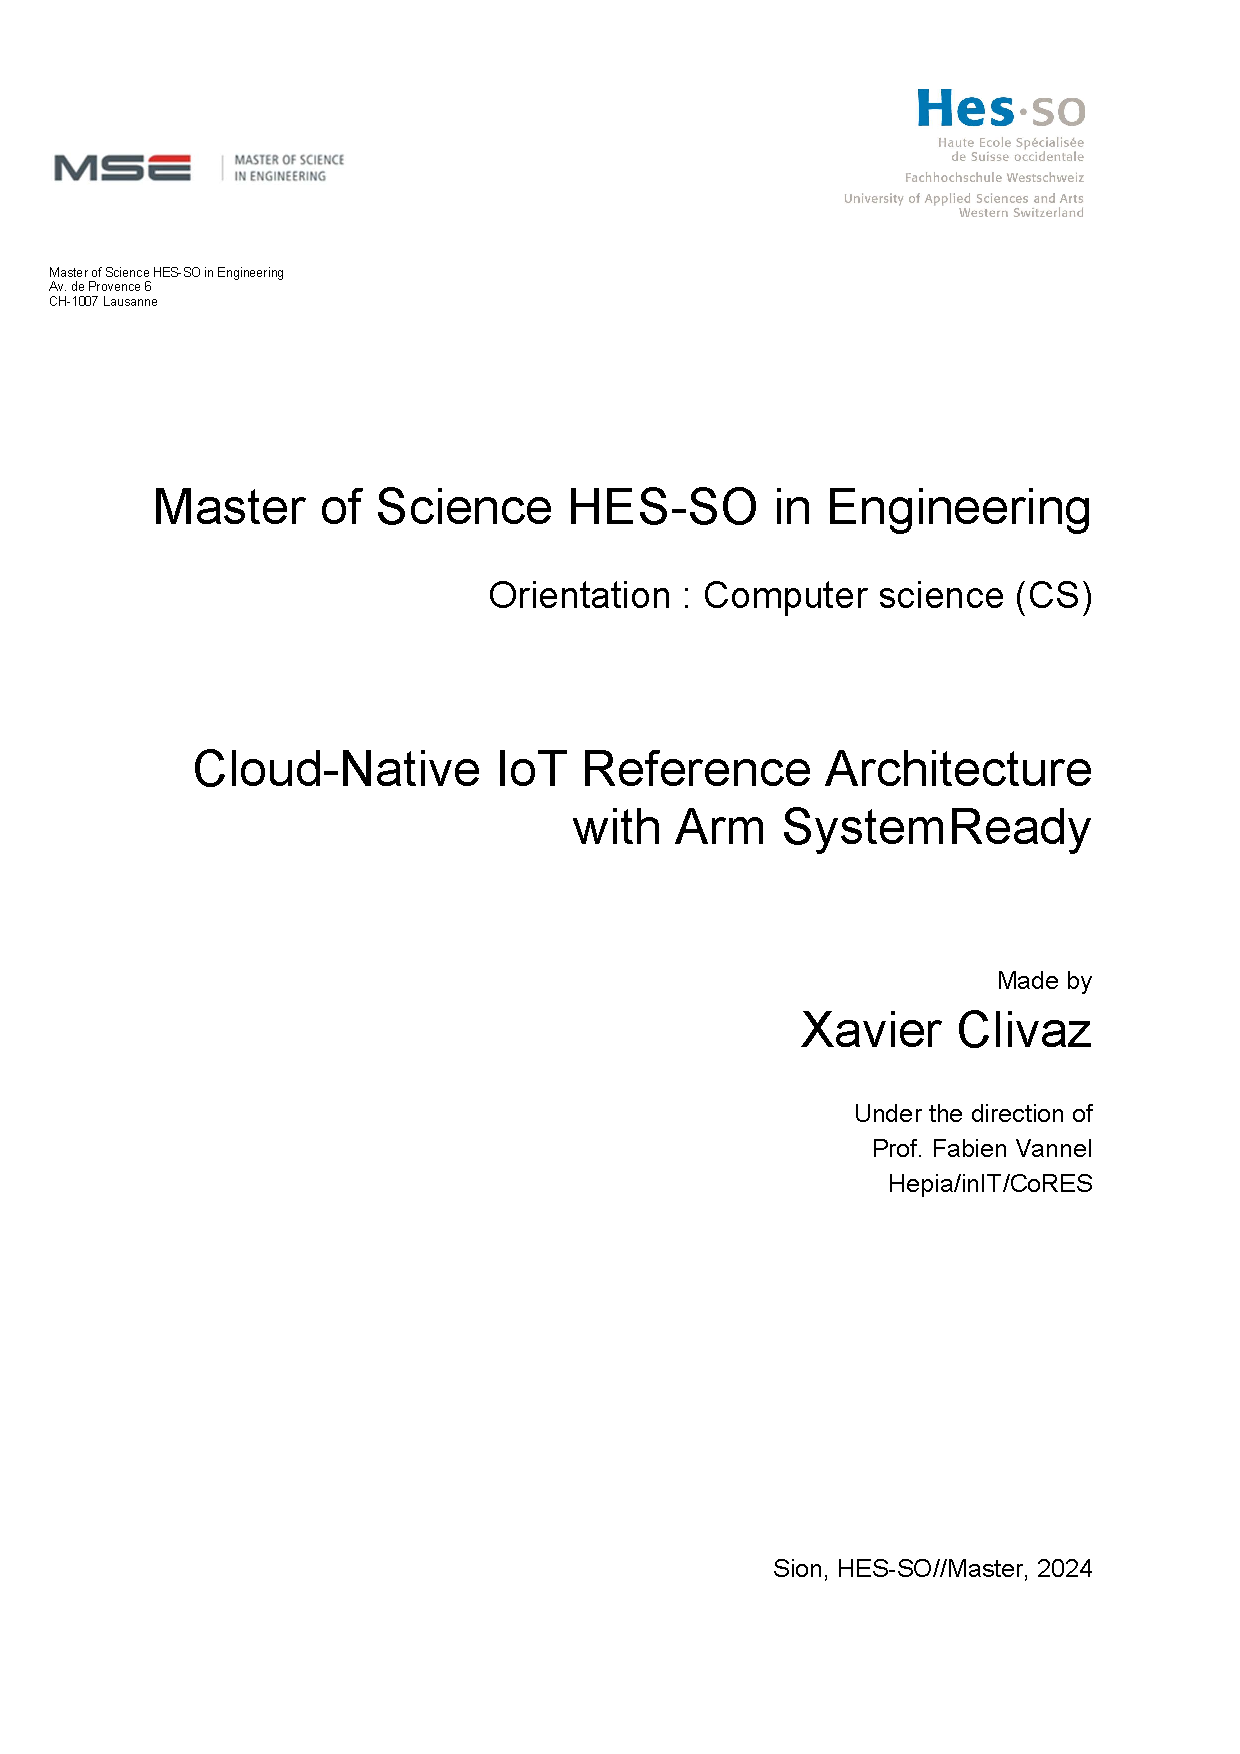
\includepdf{01-head/titlepage.pdf}
\end{titlepage}
}

\opt{pre}{
  % Page for student info and signatures
  \newpage
  \chapter*{Information about this report}

\vspace{1 cm}

\textbf{Contact Information}

\newcommand*{\email}[1]{%
    \normalsize\href{mailto:#1}{#1}\par
    }
    
\begin{tabular}{l l}
  Author:  & \Author \\
  & \AuthorDegree\,Student \\
  & \University \\
  & \Country \\
  Email: & \email{\AuthorEmail}
\end{tabular}

\vspace{1 cm}

\textbf{Declaration of honor}

{\renewcommand{\arraystretch}{2}
\begin{tabular}{p{2.5cm} p{11cm}}
  & I, undersigned, \Author, hereby declare that the work submitted is the result of a personal work. I certify that I have not resorted to plagiarism or other forms of fraud. All sources of information used and the author quotes were clearly mentioned. \\
  Place, date: & \Place, \Date \\
  Signature: & \underline{\hspace{7cm}}\hspace{-5.5cm}
\includegraphics[width=0.15\textwidth]{signature.png}
  % if you want to sign by hand on a line use the following two lines
  % Place, date: & \underline{\hspace{7cm}} \\
  % Signature: & \underline{\hspace{7cm}}
\end{tabular}
}

\vspace{\fill}

% Not used anymore since 2021
%\textbf{Validation}
%
%Accepted by the \University \, (\Country, \Place) on a proposal from:
%
%\vspace{0.5cm}
%
%\Advisor, Thesis project advisor
%
%\Expert, \ExpertLab, Main expert
%
%\vspace{1cm}
%
%Place, date: \underline{\hspace{8cm}}
%
%\vspace{3cm}
%
%{ \renewcommand{\arraystretch}{1.5}
%\begin{tabular}{p{5cm} p{7cm}}
%  \Advisor  & \Dean\\
%  Advisor   & Dean, HEI-VS//Systems Engineering\\
%\end{tabular}
%}

  % Acknowledgments (your dedication etc)
  \newpage
  % ------------------------------------------------------------------------------
% The acknowledgement section of a thesis is where you recognise and thank
% those who supported you. This can be but is not limited to individuals,
% institutions or organisations.
% ------------------------------------------------------------------------------

\chapter*{Acknowledgements}
\markboth{Acknowledgements}{Acknowledgements}
\addcontentsline{toc}{chapter}{Acknowledgements}


% -- Your text goes here --
This master's thesis would not have been written over five months without the support of a number of people. It's time to thank all these contributors, whether they are closely involved in the project or are far removed from the digital world.

\begin{itemize}
    \item [•] First of all, I would like to thank my family and especially my parents, without whom I wouldn't be able to fulfil all my dreams. So I'm always able to fulfil my potential in my daily life. It's the strength of spirit I've inherited that will always enable me to move forward despite the obstacles I encounter.
    \item [•] Secondly, I would like to thank my supervisor, Mr Fabien Vannel, who was always at my complete disposal. He was able to provide me with invaluable advice throughout the work to achieve the desired result.
    \item [•] Finally, I would like to thank everyone at \nameref{subsec:56k.cloud}. They are a great team, bringing joy and good humour to the organisation. What's more, they were able to contribute their knowledge when obstacles were encountered.
\end{itemize}

  % Abstract
  \newpage
  % ------------------------------------------------------------------------------
% One Page
% - Problem
% - Objective(s)
% - Approach and method
% - Results, Solutions (This part should have the most prominence)
% - Conclusion
% ------------------------------------------------------------------------------

\chapter*{Abstract}
\addcontentsline{toc}{chapter}{Abstract} % adds an entry to the table of contents


% -- Your text goes here --
Cloud-Native IoT Reference Architecture with Arm SystemReady is an open-source project designed to meet the integration challenges between embedded systems and the cloud. This architecture facilitates the automatic provisioning of a cloud infrastructure and the integration of a fleet of embedded systems during their initial start-up. Designed for use with AWS, it focuses on core components while leveraging Arm processors and SystemReady certifications. The project aims to streamline collaboration between embedded systems engineers and cloud professionals, allowing them to focus on their end products. By following Cloud-Native best practices, the continuous integration and delivery tools ensure a robust, functional architecture on various Arm-based and SystemReady-certified embedded systems. The ultimate aim is to encourage the creation of a community around this architecture, enabling engineers to adopt it and apply it easily to their projects. In addition, a demonstration is included involving the deployment of a cloud infrastructure on AWS and the automatic configuration of cloud services for seamless interaction with an embedded system, plus data visualisation accessible via a web interface.

\vspace{0.5cm}
\textbf{Key words:}
\Keywords

}

% Table of contents
\opt{toc}{
  \newpage
  \phantomsection
  \addcontentsline{toc}{chapter}{Contents}
  \tableofcontents
}

% List of figures
\opt{tof}{
  \newpage
  \phantomsection
  \addcontentsline{toc}{chapter}{List of Figures}
  \listoffigures
  \mtcaddchapter
}

% List of tables
% \opt{tot}{
%   \phantomsection
%   \addcontentsline{toc}{chapter}{List of Tables}
%   \listoftables
%   \mtcaddchapter
% }

% List of listings
% \opt{tol}{
%   \phantomsection
%   \addcontentsline{toc}{chapter}{List of Listings}
%   \listoflistings
% }

% Restore paragraphs
\setlength{\parskip}{1em}
	
% -----------------------------------------------------------------------------
% Main matter
% -----------------------------------------------------------------------------
\mainmatter

% Chapters
\setcounter{mtc}{4} % Help minitoc skip the front matter chapters
% ------------------------------------------------------------------------------
% Introduce the topic - What characterizes the topic?
% Introduce the goal - What do you want to achieve with your thesis?
% Make the reader curious - What motivates the reader to read on?
% Describe the relevance - Why is this bachelor thesis scientifically relevant?
%
% The introduction should have the following content:
% - Initial situation & presentation of the topic - You introduce the topic with an exciting 'bait'. You provide initial information on the topic and the object of research and explain the current state of research.
% - Relevance of the topic & motivation - You justify the relevance of your topic (scientifically) and place it in the context of your field. In addition, it is often required that you disclose your personal motivation.
% - Problem description and thematic delimitation - By means of a specific research question (or hypothesis) you present your explicit research interest. If necessary, explain technical terms.
% - Objectives - Your introduction should clearly state what the goal of your paper is and what outcome you hope to achieve upon completion of the bachelor thesis.
% - Method You explain the approach and justify the choice of method.
% - Structure of the Bachelor's thesis - Finally, you give the reader a general overview of your Bachelor's thesis by explaining the structure, showing the red thread and how the research question is answered.
% ------------------------------------------------------------------------------

\opt{never}{\addbibresource{03-tail/bibliography.bib}} % to make citation found in most IDE

\chapter{Introduction}
\label{chap:introduction}

% -- Your text goes here --
For a long time, embedded systems remained isolated from each other. Now it's time to bring them together with the world of the \gls{cloud}. Hardware devices have always been limited in terms of resources. Designs have allowed them to evolve according to their use case. However, physical limits have been observed. This is how the \hyperref[subsec:cloudcomputing]{cloud computing} came into being, partly in response to these difficulties.

The \gls{cloud} provides a huge number of advantages. It frees up hardware resources to optimise the operation of embedded systems. It is likely that these systems will not be able to perform complex calculations. The \hyperref[subsec:cloudcomputing]{cloud computing} has the capacity to do this. The storage problem is another constraint. The \hyperref[subsec:cloudcomputing]{cloud computing} offers almost unlimited storage. It doesn't stop there. It is capable of offering constant scalability to infrastructures. It is made up of different independent services that can be easily connected together. There is vertical scaling, which means increasing the size of a resource, and horizontal scaling, which means increasing the number of resources.

More and more engineers have decided to take an interest in this area in order to interconnect their embedded systems with the \gls{cloud}. This practice is an integral part of the \nameref{subsec:iot}. Due to increasingly large projects, not to mention artificial intelligence, they want to use \hyperref[subsec:cloudcomputing]{cloud computing} environments in order to no longer be constrained by resources. To make it easier to use a \gls{cloud_infrastructure}, companies have decided to offer \gls{cloud} platforms comprising a multitude of services for all types of use (\gls{aws}, Microsoft Azure, etc). It's also a way of letting engineers work on their business rather than worrying about maintaining and securing these infrastructures.


% -----------------------------------------------------------------------------
\section{56K.\Gls{cloud}}
\label{subsec:56k.cloud}

% -- Your text goes here --
\nameref{subsec:56k.cloud} is a company based in Sion (Valais) since 2018. It offers various services through the \gls{cloud}. It provides solutions for businesses that want to improve their processes while reducing their costs. It is also a consultancy firm that seeks to promote the \gls{cloud} to customers who find it difficult to understand certain concepts in this rapidly expanding digital world. Collaborations with a number of partners are also an asset, enabling us to pool a wide range of skills to provide customers with a complete product. In order to share its vision of the \gls{cloud} more widely, it has additional premises in Winterthur (Zurich).
\begin{center}
    \begingroup
    
\includegraphics[width=0.5\columnwidth]{introduction/enterprise_logo.png}
    \captionof{figure}{\nameref{subsec:56k.cloud} company logo \cite{enterprise_56k.cloud}}
    \label{fig:enterprise_logo}
    \endgroup
\end{center}
The idea of a \gls{cloud} solution is to move an on-premise infrastructure to the \gls{cloud}. It's a way of reducing costs by only paying for what you use (pay-as-you-go), and by having something that can be easily scalable. It's also a good way of increasing the speed of processes by using optimal resources for each application.

In terms of consultancy, \nameref{subsec:56k.cloud} introduces \nameref{subsec:cloudnative} technology to customers who want to find out more. It also covers the subject of \acrshort{devops} and containerisation.


% -----------------------------------------------------------------------------
\section{Problem}

% -- Your text goes here --
While \nameref{subsec:56k.cloud} mainly offers \gls{cloud} solutions, this company also works in the \acrfull{iot} sector. Recently, it quickly noticed a major problem between embedded systems engineers and those from the world of \gls{cloud}. More and more engineers are asking for devices to be able to link easily and quickly to a \gls{cloud_infrastructure}. However, there is currently no reference architecture that enables an infrastructure to be deployed and an embedded system to be provisioned directly.

This is a real problem because of the time needed and the difficulty for engineers to link hardware to a \gls{cloud_infrastructure}. Because of the two distinct professions, a person coming from the \gls{cloud} will need time to understand and set up an operating system capable of connecting to an infrastructure. And vice-versa, a person coming from the hardware world will need to familiarise themselves with a \gls{cloud_infrastructure}, not to mention setting it up while using the best practices of the \nameref{subsec:cloudnative}.
\begin{center}
    \begingroup
    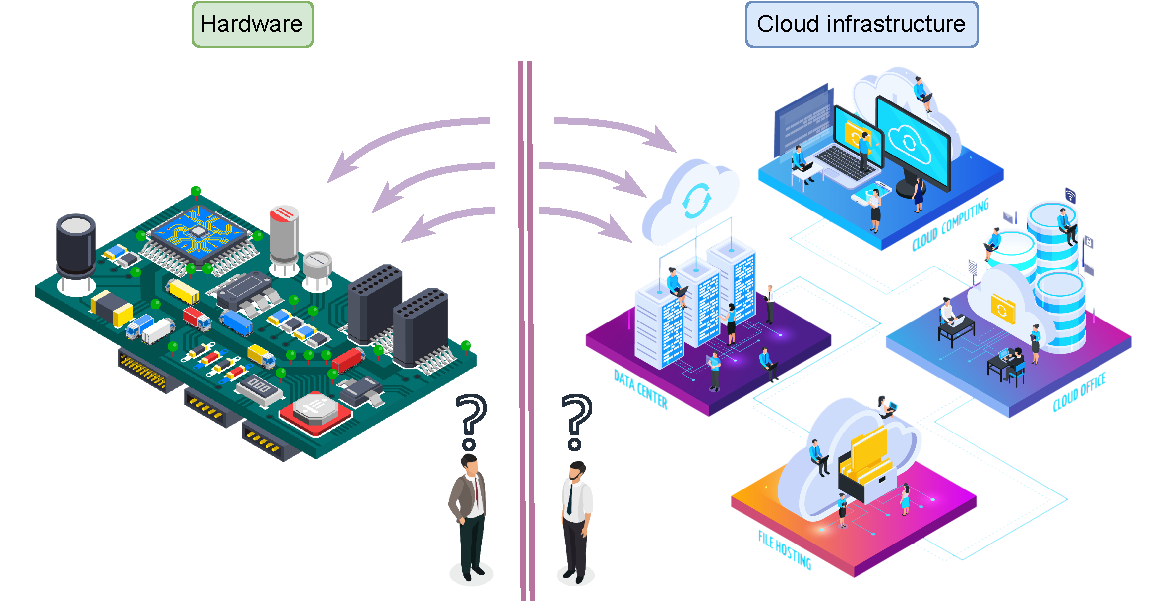
\includegraphics[width=1\columnwidth]{introduction/problem.pdf}
    \captionof{figure}{The problem of linking the hardware to the \gls{cloud_infrastructure} \cite{images_freepik}}
    \label{fig:problem}
    \endgroup
\end{center}
The need to find a solution arose when engineers started asking electronic board manufacturers to design equipment offering services for linking to a \gls{cloud_infrastructure}. Since these manufacturers are not in this discipline, they do not want to spend time developing these types of solutions. It is therefore possible to identify the main players affected. There are the hardware engineers who are unable to meet the new needs of customers. Cloud engineers, who want to do the job for them, have to devote part of their time to introducing embedded concepts. Learning something new can quickly become time-consuming.

Nevertheless, a few solutions are gradually emerging. However, these remain very closed. There is no open source reference architecture capable of satisfying a wide range of products. These solutions therefore remain highly proprietary.


% -----------------------------------------------------------------------------
\section{Objectives}

% -- Your text goes here --
The primary aim of this work is to develop a reference architecture enabling the deployment of a \gls{cloud_infrastructure} with the \gls{provisioning} of a fleet of embedded systems. The idea is to be able to automatically provision devices to the infrastructure when they are first started up. The infrastructure must contain the essential minimum of components to make the architecture as universal as possible. Since \nameref{subsec:56k.cloud} is a partner of \gls{arm}, a processor manufacturer, the embedded systems must be equipped with this. It should be added that \gls{arm} puts certifications on their components such as SystemReady. SysteamReady program guarantees that an operating system and the following software layers can function correctly in their processors. The embedded systems used in this project must be certified SystemReady. In addition, the infrastructure must be deployed on the \gls{aws} platform. This is the \gls{cloud} provider that \nameref{subsec:56k.cloud} works with.
\begin{center}
    \begingroup
    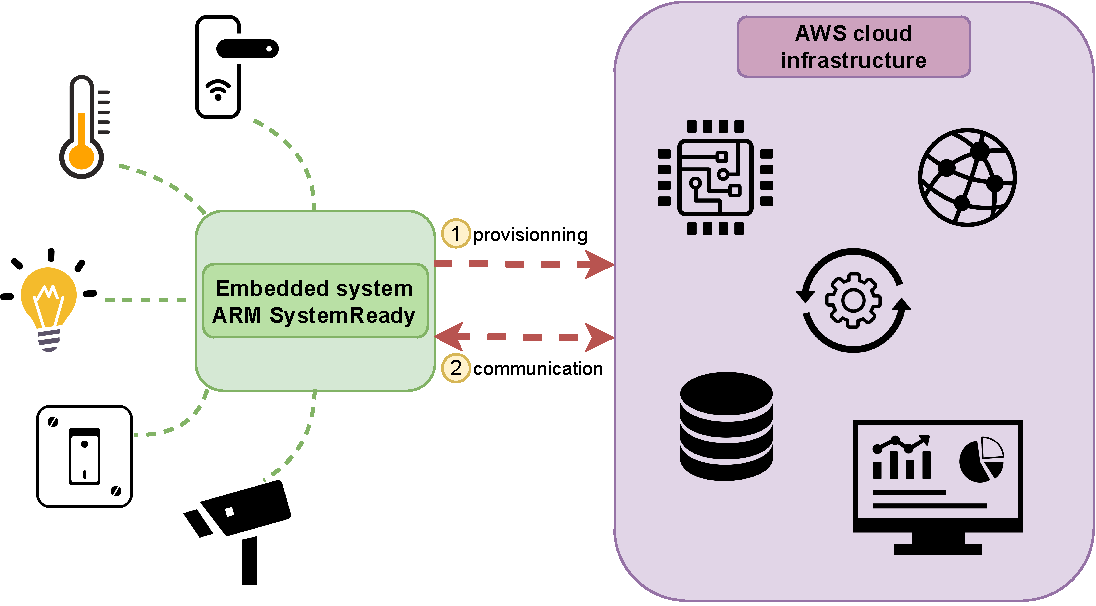
\includegraphics[width=1\columnwidth]{introduction/objective.pdf}
    \captionof{figure}{Overview of objectives}
    \label{fig:objective}
    \endgroup
\end{center}
The aim of this project is to be open source so that a community can form around it. It should enable embedded systems and \gls{cloud} engineers to use this reference architecture easily. They need to be able to focus on their final product. The best practices of \nameref{subsec:cloudnative} must be used for the development of this project. In order to guarantee a sound architecture, the use of \acrfull{ci} and \acrfull{cd} tools are essential. In addition, to ensure compatibility, the architecture must be functional on different embedded systems with a \gls{arm} processor and certified SystemReady.

Secondly, once the reference architecture is functional, a demonstration project must be based on it. This is a proof of concept. The general idea is to deploy a \gls{cloud_infrastructure} on \gls{aws} and have various \gls{cloud} services automatically set up to interact with the embedded system. Data will then transit between these two worlds and it must be viewable from an interface.


% -----------------------------------------------------------------------------
\section{Project plan}

% -- Your text goes here --
Figure \ref{fig:work_packages} shows the project plan in the form of \glspl{work_package}.
\begin{center}
    \begingroup
    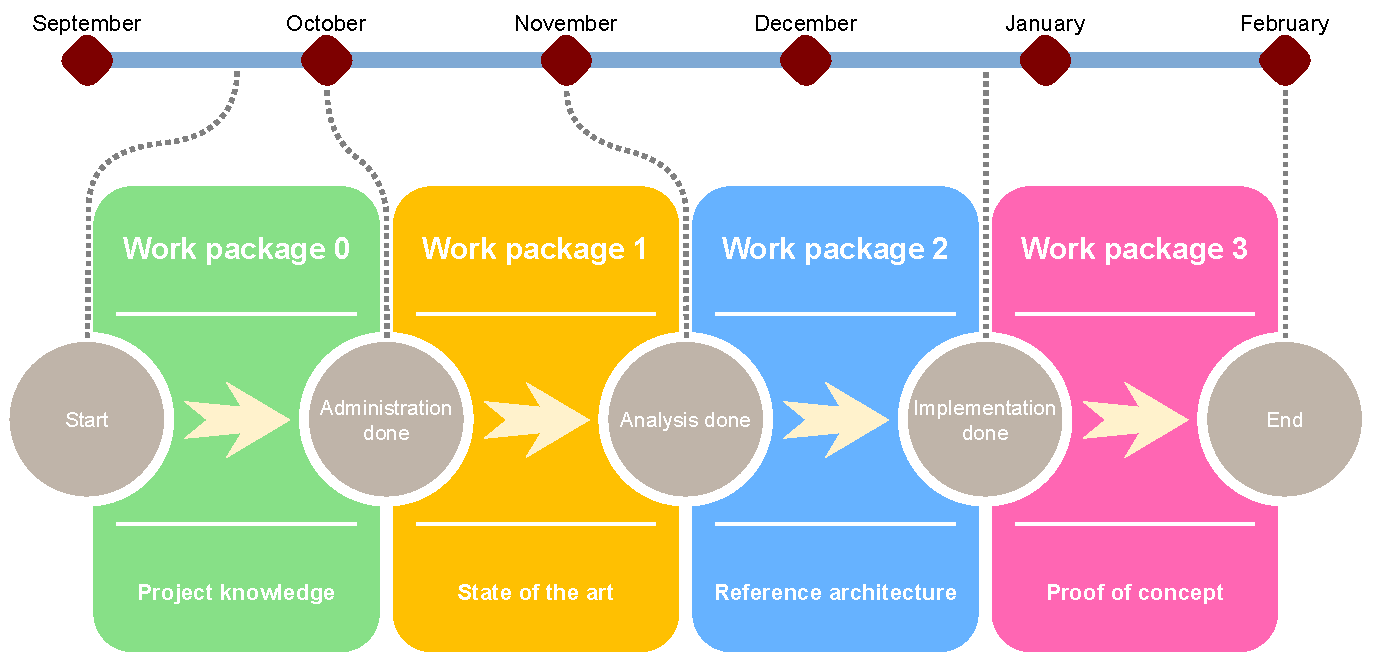
\includegraphics[width=1\columnwidth]{introduction/work_packages.pdf}
    \captionof{figure}{Project plan}
    \label{fig:work_packages}
    \endgroup
\end{center}
The first \gls{work_package} contains all the administration. It involves learning about the project, being aware of the issues and clearly defining the specifications. This takes around two weeks.

About a month is spent researching existing solutions that are closest to the project. This involves drawing up a state of the art by researching scientific articles and other documentation.

The third \gls{work_package} concerns the reference architecture. Almost two months are devoted to this. This implementation part will be the final product, which will be delivered as open source on a shared repository.

In order to validate this architecture, a proof of concept will be carried out. This is the final \gls{work_package}. It will take just over a month. Tests will be carried out to prove that it works properly.

% -----------------------------------------------------------------------------
\section{Research methodology}

% -- Your text goes here --
The research methodology used in this thesis was first to draw up a state of the art on existing solutions that are as close as possible to this project. An overview of the reference architecture was then drawn up with a view to implementing it more easily. A choice of development tools was also made. At the same time, the implementation was designed. Finally, the results were validated by means of a proof of concept.

The agile methodology, known as \gls{scrum}, was used throughout the project. It allows for iterative project management. Weekly meetings were arranged with the professor in charge of the project and, optionally, with some of the company's staff. To enable the project to progress efficiently, the \gls{kanban} method was used. This consists of virtual cards, each referring to a task. These cards are categorised in a table to determine the progress of each task. It's also a way of dividing the project into smaller parts so that time can be better estimated over the course of the project.


% -----------------------------------------------------------------------------
\section{Structure of this report}

% -- Your text goes here --
The \ref{chap:methodology} chapter (\nameref{chap:methodology}) contains a number of project methodologies for effective project management. The tools used are also described.

The \ref{chap:analysis} chapter (\nameref{chap:analysis}) contains several definitions and the state of the art. These are definitions of important terms that make up the project. The state of the art concerns the existing solutions that are closest to this project.

The \ref{chap:design} chapter (\nameref{chap:design}) contains an overview of the implementation as well as ... \colorbox{red}{To be completed}

The \ref{chap:implementation} chapter (\nameref{chap:implementation}) contains ... \colorbox{red}{To be completed}

The \ref{chap:validation} chapter (\nameref{chap:validation}) contains the analysis and validation of the results of the implementation.

The \ref{chap:conclusions} chapter (\nameref{chap:conclusions}) concludes the thesis by outlining the current state of the research, the problems encountered and future steps.
% ------------------------------------------------------------------------------
% It describes the knowledge about the studied matter through the analysis of
% similar or related published work.
% It provides a comprehensive overview of what was done, what has been done in
% the field and what should be further investigated.
% ------------------------------------------------------------------------------

\opt{never}{\addbibresource{03-tail/bibliography.bib}} % to make citation found in most IDE

\chapter{Analysis}
\label{chap:analysis}

% -- Your text goes here --
The analysis begins by explaining the fundamental concepts that are being worked on throughout the project. Next, a state of the art is provided on the various tools, methods and technologies used in \hyperref[subsec:cloudcomputing]{cloud computing} and \acrshort{iot}.

\minitoc
\newpage

% ------------------------------------------------------------------------------
\section{Definitions}
Before going into more detail on the subject of this work, it is important to look at the definitions of the various terms frequently used.

% -- Your text goes here --
\subsection{Reference architecture}
\label{subsec:ref_arch}
A reference architecture is a solution model in a specific domain. It must be built so that an architecture can be established on its foundations, to make the task of software developers easier.

The aim is to generalise a solution that shows how it works from an overview. It must be possible to observe the relationships and their interactions between the multiple components of the application based on the reference architecture. There are different layers of abstraction depending on the field of application. A high level of abstraction means that it will be possible to understand the solution through more abstract elements such as the general components that will consolidate the application, for example. A low level of abstraction means that the solution will be more precise and certainly more specific to a use case. It will be possible to find detailed relationships between the services contained in the general components.

\subsection{\texorpdfstring{\Gls{cloud}}{} computing}
\label{subsec:cloudcomputing}
The National Institute of Standards and Technology (NIST) \cite{nist_definition_cloud_computing} has standardised the definition of \hyperref[subsec:cloudcomputing]{cloud computing} as follows:
\begin{quote}
    \textit{Cloud computing is a model for enabling ubiquitous, convenient, on-demand network access to a shared pool of configurable computing resources (e.g., networks, servers, storage, applications, and services) that can be rapidly provisioned and released with minimal management effort or service provider interaction. \cite{nist_definition_cloud_computing}}
\end{quote}
It is added in the article \cite{nist_definition_cloud_computing} that this model of \gls{cloud} consists of three service models and four deployment models. The service models are as follows:
\begin{itemize}
    \item[—] \acrfull{iaas} : The capability offered to the consumer consists of providing processing, storage, network and other fundamental computing resources where the consumer can deploy and run arbitrary software, which may include operating systems and applications. The consumer manages the operating systems, storage and applications.
    \item[—] \acrfull{paas} : The capacity provided to the consumer consists of deploying on the \gls{cloud_infrastructure} applications created or acquired by the consumer using programming languages, libraries, services and tools supported by the provider. The consumer manages only the applications and storage.
    \item[—] \acrfull{saas} : The consumer has the option of using the supplier's applications running on a \gls{cloud_infrastructure}. The consumer manages nothing of the infrastructure apart from any configuration of the applications.
\end{itemize}
\begin{center}
    \begingroup
    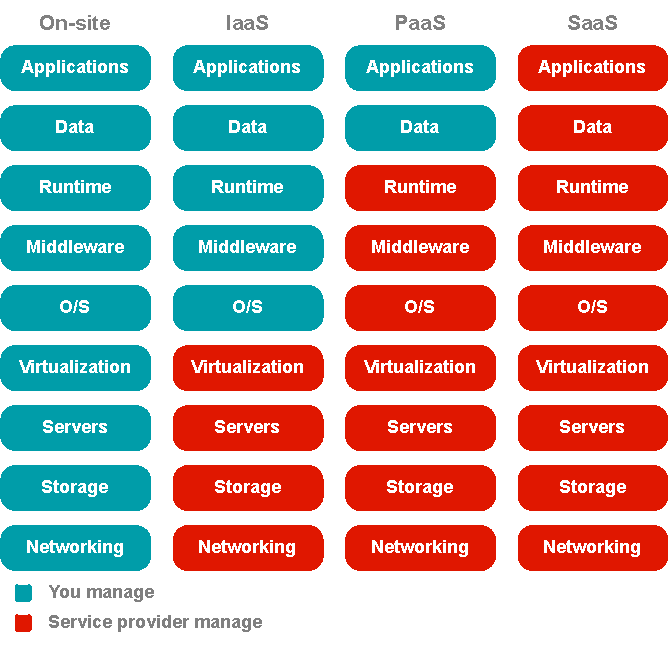
\includegraphics[width=.7\columnwidth]{analysis/iaas_paas_saas.pdf}
    \captionof{figure}{Comparison of different service models \cite{iaas_paas_saas}}
    \label{fig:iaas_paas_saas}
    \endgroup
\end{center}
The deployment models are as follows \cite{nist_definition_cloud_computing} :
\begin{itemize}
    \item[—] \textbf{Private \gls{cloud}} : The \gls{cloud_infrastructure} is made available for exclusive use by a single organisation comprising multiple consumers. It may be owned, managed and operated by the organisation, by a third party or by a combination of both, and it may exist on the organisation's premises or off-site.
    \item[—] \textbf{Community \gls{cloud}} : The \gls{cloud_infrastructure} is reserved for the exclusive use of a specific community of consumers from organisations with common concerns. It may be owned, managed and operated by one or more organisations within the community, by a third party or by a combination of such organisations, and it may exist on or off premises.
    \item[—] \textbf{Public \gls{cloud}} : The \gls{cloud_infrastructure} is made available to the general public for open use. It may be owned, managed and operated by a business, educational institution or government organisation, or a combination of these. It is located on the provider's premises.
    \item[—] \textbf{Hybrid \gls{cloud}} : The \gls{cloud_infrastructure} is a composition of two or more distinct infrastructures (private, community or public) which remain unique entities, but which are linked by a standardised or proprietary technology that allows the portability of data and applications.
\end{itemize}

\subsection{\Gls{cloud}-Native}
\label{subsec:cloudnative}
\nameref{subsec:cloudnative} is an approach to software development which aims to design, implement and manage applications in the \gls{cloud}. \nameref{subsec:cloudcomputing} environments will be necessary for the proper execution of workloads.

The infrastructure can be deployed in private, public or hybrid \glspl{cloud}. This approach will enable the development of modern, easily scalable applications. The flexibility aspect is also emphasised thanks to techniques for decoupling the multiple services of an application. Another strength of the \gls{cloud} is its reliability and sustainability. Since the number of resources is incalculable and they are distributed around the world, redundancy guarantees security in the event of an incident, with almost instantaneous migration of an application's execution. The customer is therefore very often spared any unforeseen events. It is also possible to provide updates in real time and on a recurring basis.

The main benefits are high efficiency, reduced costs and high availability. Applications will be able to exploit resources that are optimal for their use case. The term pay-as-you-go is widely used, as the cost will depend solely on the use made of the resources and not on anything else, such as their maintenance, hardware security, etc. Availability is high because of the astronomical number of resources made available by the various \gls{cloud} environment providers.

\subsection{\acrlong{iot}}
\label{subsec:iot}
\acrfull{iot} refers to the interconnection between physical objects and the internet. Objects can range from light bulbs to medical devices and much more. The main areas concerned are home automation and medical technology.

This involves linking different objects and applications to move into an automated world. As this becomes more and more widespread, the services needed to make it work need a huge amount of resources. This has been made possible by the \gls{cloud}. Everything must be accessible from anywhere in the world, quickly and securely. Several communication technologies are possible to guarantee excellent accessibility and reliability.

% ------------------------------------------------------------------------------
\section{Problem formulation}

% -- Your text goes here --
The general question for analysis is: "Which technologies should be used to develop a reference architecture".

To help answer this question, it is important to consider the following aspects:
\begin{itemize}
    \item[—] Technology
    \item[—] Environment
    \item[—] Tools
    \item[—] Certification
\end{itemize}
Since the development uses the \nameref{subsec:cloudnative} approach, its history can be described first. The integration of the \acrshort{iot} world into \hyperref[subsec:cloudcomputing]{cloud computing} must then be observed through various scientific works and research. A study of \gls{cloud} service providers must be undertaken to differentiate the iot services offered by each one. As the reference architecture is based on an \acrfull{iac}, research into \acrshort{iac} tools is carried out. Finally, it is worth finding out whether SystemReady certification exists for electronic boards using an \gls{arm} processor architecture.


% ------------------------------------------------------------------------------
\section{Literature search}

% -- Your text goes here --
Literature search has focused on academic search engines. The following search engines were used :
\begin{itemize}
    \item[—] \href{https://scholar.google.com}{Google Scholar}
    \item[—] \href{https://ieeexplore.ieee.org/Xplore/home.jsp}{IEEE Xplore}
    \item[—] \href{https://www.sciencedirect.com}{ScienceDirect}
\end{itemize}
The sources were mainly conference papers. Some information was found on websites. The following keywords were used to find sources that met the requirements of this analysis:
\begin{itemize}
    \item[—] integration
    \item[—] embedded systems
    \item[—] \acrshort{iot}
    \item[—] \nameref{subsec:cloudnative}
    \item[—] \gls{cloud}
    \item[—] \hyperref[subsec:cloudcomputing]{cloud computing}
    \item[—] \gls{cloud} providers
    \item[—] \gls{cloud} platforms
    \item[—] \acrlong{iac}
    \item[—] \acrshort{iac} tools
    \item[—] \nameref{sec:arm_systemready}
\end{itemize}


% ------------------------------------------------------------------------------
\section{History of the \texorpdfstring{\nameref{subsec:cloudnative}}{} approach}

% -- Your text goes here --
\nameref{subsec:cloudnative} is a term that has been around for several years. Figure \ref{fig:google_trend_cloud} shows the evolution of this term since 2006. The boom took place around 2016. It is undoubtedly due to the birth of Docker (2013) \cite{docker} and Kubernetes (2014) \cite{k8s}. In 2015, the Cloud Native Computing Foundation \cite{cncf} was created with the aim of making the \nameref{subsec:cloudnative} approach ubiquitous \cite{cncf_charter}.
\begin{center}
    \begingroup
    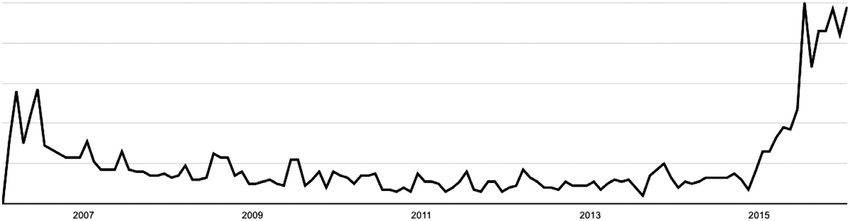
\includegraphics[width=1\columnwidth]{analysis/google_trend_cloud-native.png}
    \captionof{figure}{Google trends (01.01.2006 until 22.05.2016) of term \nameref{subsec:cloudnative} \cite{understanding_cloud_native}}
    \label{fig:google_trend_cloud}
    \endgroup
\end{center}
Before all this, there were only on-site data centres. Generally speaking, each company had its own servers running in its own data centre. This meant that servers were always set up for a specific application. \cite{history_cloud_native}

\subsection{The virtualisation}
The first change came in the 2000s with the virtualisation of servers, although this has been around since the 1960s. When a new application had to be developed, new physical servers had to be bought. With virtualisation, it is no longer necessary to buy new ones. It is possible to run several applications on the same server using virtualisation, which limits the hardware resources for each application (figure \ref{fig:virtualisation}). \cite{history_cloud_native}
\begin{center}
    \begingroup
    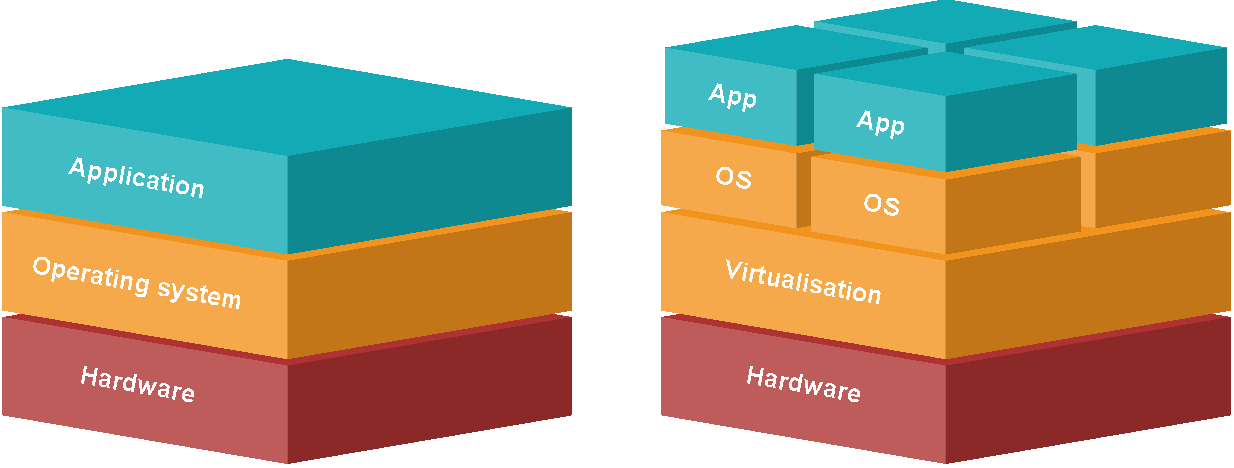
\includegraphics[width=1\columnwidth]{analysis/virtualisation.pdf}
    \captionof{figure}{Traditional server (left) and virtualisation (right)}
    \label{fig:virtualisation}
    \endgroup
\end{center}

\subsection{The hybrid}
Despite this, a minimum of one server had to be purchased for an application to work. There were also resource limits for a certain number of applications. Unfortunately, not everyone could afford to buy new servers. In 2006, \gls{aws} launched three web services, \acrfull{ec2}, Simple Storage Service (S3) and Simple Queue Service (SQS), to allow organisations and individuals to use Amazon's IT infrastructure on an as-needed basis at basic prices \cite{evaluation_aws_services}. This initiative stems from a restructuring of the Amazon platform for better scalability and this has made it possible to sell virtual servers as a service \cite{ec2_origins}. By extension, the myth of making money from servers not in use for the majority of the year has been debunked by Benjamin Black, co-founder of the \acrshort{ec2} \cite{ec2_origins}. This is where the world of \gls{cloud} really began. Kratzke and Quint confirm this in their scientific article \cite{understanding_cloud_native}. The purpose of the \acrshort{ec2} service, which is still used today, is to offer a virtual machine in the \gls{cloud}. This is a \hyperref[subsec:cloudcomputing]{cloud computing} environment for running workloads. It is now possible to migrate your infrastructure from the database to the \gls{cloud}. The corresponding expression is "Lift and Shift" \cite{ibm_lifAndShift}. These were undoubtedly the first so-called \nameref{subsec:cloudnative} approaches \cite{history_cloud_native}. However, this term only appeared in papers for the first time in 2012 \cite{understanding_cloud_native}. These were two conference papers proposing solutions for \nameref{subsec:cloudnative} applications \cite{closer12, 4caast}. Organisations have learned a lot about only paying for what you use. From there, there's a move to hybrid where companies are still using their on-premises servers alongside servers in the \gls{cloud}. \cite{history_cloud_native}

\subsection{All to the \texorpdfstring{\gls{cloud}}{}}
A new barrier has now been crossed. It's no longer a question of doing hybrid, but of transferring the entire infrastructure to the \gls{cloud}. This was made possible when \gls{cloud} service providers such as \gls{aws}, Microsoft Azure, Google Cloud and many others developed several services for all types of use. The reason there are different services is quite simply to decouple application functionality as much as possible. This is known as a microservices architecture. The risk of an entire application being interrupted in the event of a problem is much less likely. However, some organisations still have applications that are several decades old and have a monolithic architecture. It is not necessarily possible to decouple functionalities. That's why they work on a hybrid basis. \cite{history_cloud_native}

\subsection{The \texorpdfstring{\nameref{subsec:cloudnative}}{} approach}
If we ask several engineers today about the definition of the \nameref{subsec:cloudnative} approach, we will find varying interpretations. There are currently three main schools of thought on this subject \cite{history_cloud_native}. The first group considers that an approach is \nameref{subsec:cloudnative} when all the workloads run in the \gls{cloud}. A minority within this group argue that you can be partially \nameref{subsec:cloudnative}, i.e. have one complete application deployed in the \gls{cloud} while maintaining another application locally. However, others feel that this is still a hybrid approach. A second group says that to be truly \nameref{subsec:cloudnative}, you need to fully exploit the capabilities offered by the \gls{cloud}. This means not only using the basic services of a \gls{cloud} provider, but also making full use of the advanced features on offer, such as serverless functions. Some even consider that a company has to be born in the \gls{cloud} to be truly \nameref{subsec:cloudnative}, a phenomenon that is increasingly being observed, with companies launching their first applications directly in the \gls{cloud} without ever having used on-premises servers. This is the case for the company \nameref{subsec:56k.cloud} \colorbox{red}{To be confirmed}. \cite{history_cloud_native}

In 2018, a brief history of \gls{cloud} application architectures described the term \nameref{subsec:cloudnative} as follows :
\begin{quote}
    \textit{\Glspl{cloud_infrastructure} (\acrshort{iaas}) and platforms (\acrshort{paas}) are built to be elastic. Elasticity is understood as the degree to which a system adapts to workload changes by provisioning and de-provisioning resources automatically. Without this, \hyperref[subsec:cloudcomputing]{cloud computing} is very often not reasonable from an economic point of view. Over time, system engineers learned to understand this elasticity options of modern \gls{cloud} environments better. Eventually, systems were designed for such elastic \glspl{cloud_infrastructure}, which increased the utilization rates of underlying computing infrastructures via new deployment and design approaches like containers, microservices or serverless architectures. This design intention is often expressed using the term \nameref{subsec:cloudnative}. \cite{history_cloud_application}}
\end{quote}


% ------------------------------------------------------------------------------
\section{Integrating \texorpdfstring{\hyperref[subsec:cloudcomputing]{cloud computing}}{} with \texorpdfstring{\acrshort{iot}}{} embedded systems}

% -- Your text goes here --
With technology advancing at a rapid pace, today's world appreciates help in making everyday life better \cite{state_of_the_art_integration_iot_cloudComputing}. Embedded systems that have become increasingly connected now offer this service. However, since they need to attend any location for any domain and task, they need to be small for better integration. As a result, resources are limited for computing operations, data storage, data processing and so on. The built-in security and low energy consumption that these devices must also ensure are not enough to allow them to move forward. This is why \hyperref[subsec:cloudcomputing]{cloud computing} needs to be integrated to fill the gaps left by \acrshort{iot} \cite{state_of_the_art_integration_iot_cloudComputing}. Cloud of Things is one of the paradigms given to the combination of these two technologies in 2014 \cite{cloud_of_thing}.

\subsection{Overview}
A model for integrating \hyperref[subsec:cloudcomputing]{cloud computing} into an embedded system is shown in figure \ref{fig:device_and_cloud_computing}. \cite{integration_embedded_systems_cloudComputing}
\begin{center}
    \begingroup
    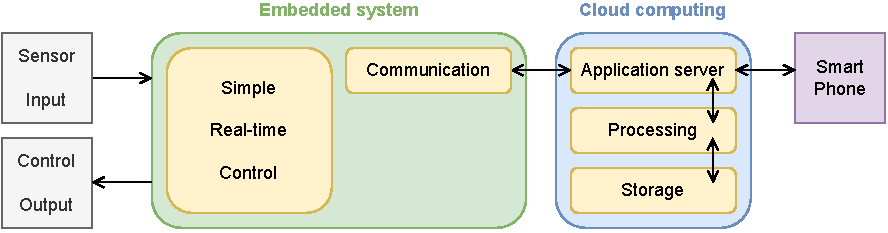
\includegraphics[width=1\columnwidth]{analysis/device_and_cloud_computing.pdf}
    \captionof{figure}{Model for integrating \hyperref[subsec:cloudcomputing]{cloud computing} into an embedded system \cite{integration_embedded_systems_cloudComputing}}
    \label{fig:device_and_cloud_computing}
    \endgroup
\end{center}
The main idea is to use only what is necessary on the \acrshort{iot} device. In other words, all computing and storage functions should be moved to the \gls{cloud}. The device should only be linked to the input and output peripherals using a simple controller and establish communication with the \gls{cloud}. For the integration to work, the embedded system must have an internet connection. \hyperref[subsec:cloudcomputing]{Cloud computing} would contain the core of the application as well as various services to perform analysis, processing and calculation operations, and store data in real time. From there, it would also be possible to view the data from a smartphone. This approach is a solution that was thought up by Furuichi and Yamada in 2014 \cite{next_generation_iot_cloud}. It offers a number of advantages, such as reduced energy consumption by eliminating large workloads and reduced size by freeing up electronic components. The \gls{cloud} also makes it easy to scale up if necessary. The application can then be highly scalable. \cite{integration_embedded_systems_cloudComputing}

Furuichi and Yamada wanted to use a project to prove that their suggested approach worked. They developed a traffic jam detection system that recognises car licence plate numbers along with their location and time. For a plate number to be recognised from a raw image, image processing is carried out using machine learning. They found that this application, split between an \acrshort{iot} device and a \hyperref[subsec:cloudcomputing]{cloud computing} environment, scored much better than the same application managed entirely on a laptop or embedded system. The evaluation looked at cost, battery life, performance, scalability and reliability. \cite{next_generation_iot_cloud}

\subsection{Reference architecture}
A reference architecture has been developed to support \acrshort{iot} objects in \hyperref[subsec:cloudcomputing]{cloud computing} (figure \ref{fig:reference_architecture_CSCC}). The Standards Development Organization has decided to make this a standard by launching the Cloud Standards Customer Council programme to drive forward the adoption of \hyperref[subsec:cloudcomputing]{cloud computing}. In this architecture, various aspects are taken into account: scalability, security, reliability and protection of privacy. \cite{reference_architecture_cloud_iot}
\begin{center}
    \begingroup
    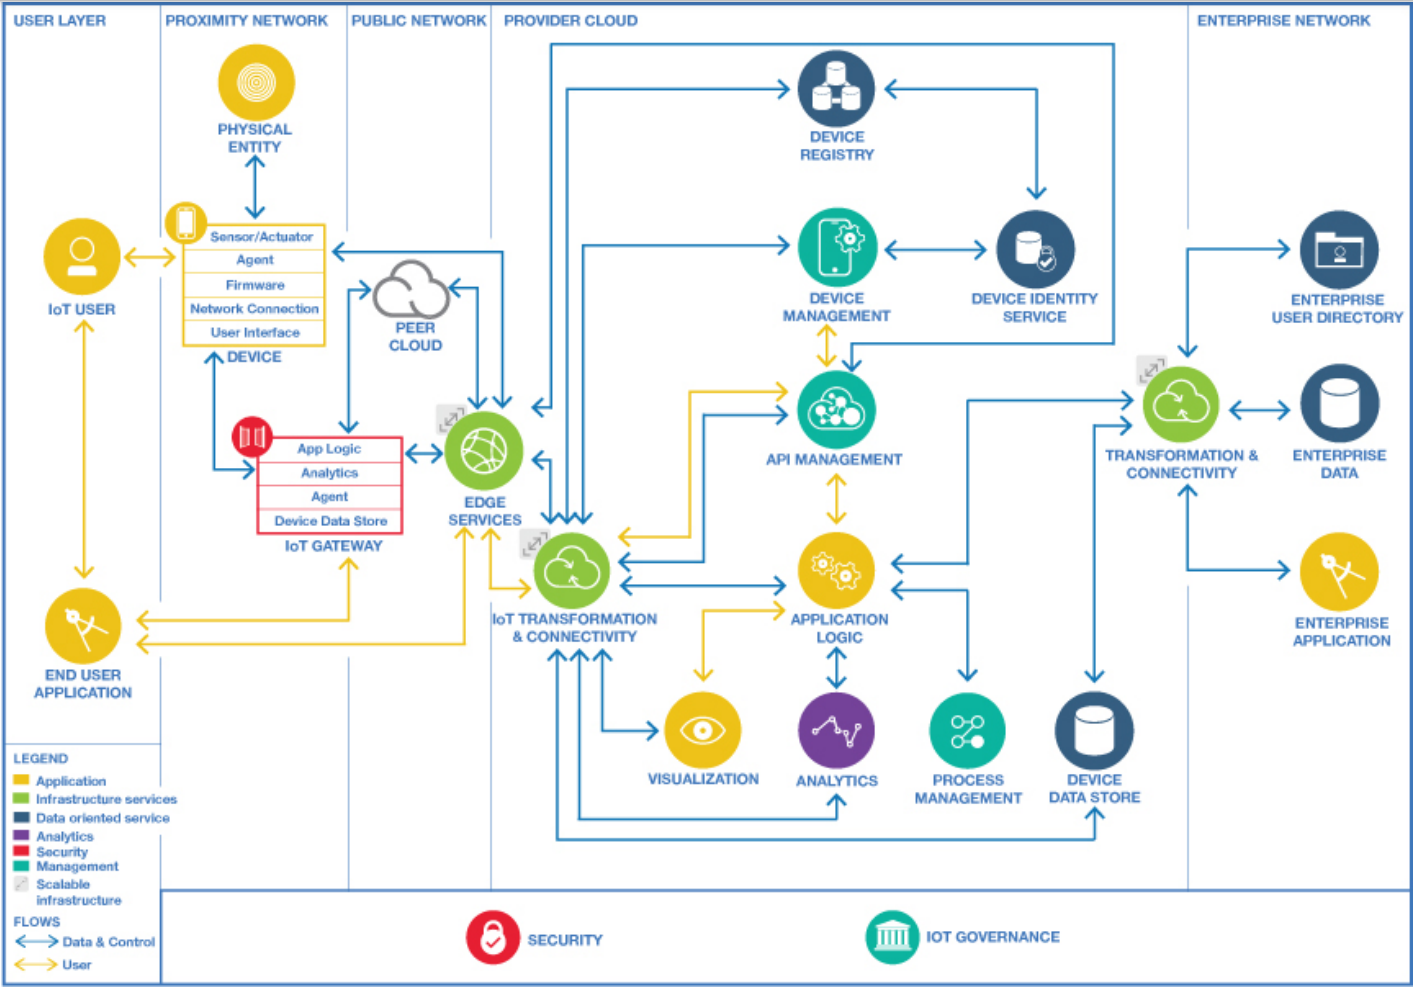
\includegraphics[width=1\columnwidth]{analysis/reference_architecture_CSCC.png}
    \captionof{figure}{Cloud Customer Reference Architecture for IoT \cite{reference_architecture_cloud_iot}}
    \label{fig:reference_architecture_CSCC}
    \endgroup
\end{center}
The architecture proposed in figure \ref{fig:reference_architecture_CSCC} is made up of components and their relationships. They are separated under a three-tier architecture model, called 3-Tier (presentation, logic, data). There is edge-tier, the platform tier and the enterprise tier.

The edge-tier contains the "Proximity Network" and "Public Network" parts. It represents the place where data is collected. It is collected from an \acrshort{iot} device in a proximity network. The data will either be sent to an \acrshort{iot} gateway or directly to the \gls{cloud} provider.

The \gls{cloud} provider tier manages the entire logical part of the application. It includes the collection, processing and analysis of data flows. Each device is also managed in this tier, as is its identity, for example.

The enterprise tier contains the "Enterprise Network" part. It includes the enterprise data and the application. Data from \hyperref[subsec:cloudcomputing]{cloud computing} can be stored in enterprise data.

\subsection{Existing problems and solutions linked to integration}
Integrating \acrshort{iot} and \hyperref[subsec:cloudcomputing]{cloud computing} poses a number of challenges. They are to be found both on the hardware side and in the \gls{cloud}. \cite{cloud_of_thing}

There are many communication protocols. There are protocols for every type of use. On the \acrshort{iot} side, for example, there are Zigbee \cite{zigbee}, Bluetooth and \acrfull{ble} \cite{bluetooth}, LoRaWAN (long range) \cite{lora_alliance}, \acrshort{wifi}, Thread \cite{thread} and the latest Matter protocol \cite{matter}. In an \acrshort{iot} network, there can be a multitude of sensors linked to a gateway. Interoperability is a problem in this case. Since 2022, version 1.0 of the Matter protocol has been published to address this problem. However, few devices are yet compatible. In research projects, Zigbee is very popular \cite{state_of_the_art_integration_iot_cloudComputing, cloud_of_thing, secure_integration_iot_cloud_computing, smart_home_integration}. Two main technologies are used for communication between the \acrshort{iot} gateway and the \gls{cloud}: \acrfull{mqtt} \cite{mqtt} and \acrfull{coap} \cite{coap_whitepaper}. Several projects have used \acrshort{coap} for resource reasons \cite{cloudthings, actinium_integration_solution, aws_arm_architecture_iot}. It is a protocol dedicated to constrained devices with small amounts of memory \cite{coap_whitepaper}, using \acrshort{udp}. It is also suitable for devices that need to bind to web services as it uses the \acrfull{rest} model. \acrshort{rest} is an architectural style for web services \cite{cloudthings}. It would have been possible to use the \acrfull{soa} style, but it is less suited to this use case \cite{cloudthings}. Service-based architecture styles allow a high degree of decoupling from the application. This is an advantage in the event of a problem with a service, so as not to completely freeze the application. Finally, \acrshort{mqtt} is specially designed for \acrshort{iot} \cite{mqtt}. It uses the \acrshort{tcp} transport protocol. \Gls{cloud} provider \gls{aws} adopts the \acrshort{mqtt} protocol in its \acrshort{iot} sector \cite{mqtt_aws}. A communication between an \gls{arm} microcontroller and \gls{aws} proved that this protocol works \cite{aws_arm_architecture_iot}. In fact, the data passing through is often in \acrfull{json} format \cite{integration_embedded_systems_cloudComputing, smart_home_integration, itaas_reference_architecture}. This is a lightweight data representation syntax for storing and exchanging textual information \cite{smart_home_integration}. There is also the \acrfull{http} communication protocol. It would be suitable for updating \acrshort{iot} devices. It allows more bytes to be sent per packet, which increases the update speed. Furthermore, in industry, \acrshort{http} is generally less constrained by firewalls than \acrshort{mqtt} or \acrshort{coap} \cite{OTA_Solution_proposed}.

A lot of energy is consumed in \acrshort{iot} devices. The reason for this is the increasing amount of data being transferred to the \gls{cloud}. Energy needs to be managed efficiently, for example by setting a sleep mode. If this is not possible, natural energy could be used to provide power, such as solar, wind or vibration. \cite{cloud_of_thing}

Resource allocation is another debate. Each \acrshort{iot} object may have a different function. They do not necessarily require the same resources in the \gls{cloud}. What's more, unexpected events could occur requiring a greater workload. The requirements could not necessarily be predictable. Even if they were, the cost of increasing unused resources for most of the time would be a loss. \Gls{cloud} service providers offer a number of solutions to this problem. For example, \gls{aws} offers a service that balances the load in the \hyperref[subsec:cloudcomputing]{cloud computing} environment \cite{elb_aws}. The combinatorial auction approach is popular for resource allocation in the \gls{cloud} \cite{optimization_resources_allocation}. It must satisfy \acrfull{qos} constraints and maximise the \gls{cloud} provider's profit. Provider and user profit, resource utilisation and quality of service are the dominant performance factors. Research has succeeded in optimising this approach \cite{optimization_resources_allocation}. Nevertheless, as soon as a new \acrshort{iot} node is added, a sample of data could be sent to the \gls{cloud} to set up the minimum resources required. \cite{cloud_of_thing}

Identity management in an internet network is very important to ensure that each device is unique. Given the number of \acrshort{iot} devices today, IPv6 addressing would be the optimal solution. It would be sufficient to support this type of network. However, deployment remains problematic. The coexistence of IPv6 with IPv4 is not so easy \cite{cloud_of_thing}. There are three possible techniques for cooperation between the two \cite{coexistence_ipv4_ipv6}. The \acrshort{iot} device may support both types of addressing. Alternatively, IPv6 packets must be encapsulated in IPv4 packets, or a \acrfull{nat} must be available that translates both types of packet.

The discovery of new \acrshort{iot} devices to be integrated into the \gls{cloud} needs to be managed. At any time, a device can be part of a service and leave it. It is also necessary to monitor its status once it is connected and keep it up to date. \gls{aws} has developed a solution to this which must be installed on \acrshort{iot} devices. From there, the devices can be easily integrated. In addition, it is possible to perform \acrfull{ota} updates \cite{ota_aws_iot} and monitor the state of devices \cite{status_aws_iot}. Azure also provides these different services \cite{ota_azure_iot, status_azure_iot}. An update method was designed in this area in 2022 \cite{OTA_Solution_proposed}. It is based on the standard update architecture for \acrshort{iot} \cite{firmware_update_architecture_iot}, proposed by the Internet Engineering Task Force (IETF).

\hyperref[subsec:cloudcomputing]{Cloud computing} environments must respond correctly to data flows, whether large or small. The urgency with which certain data is transmitted is also an integral part of this \acrshort{qos}. \acrshort{qos} is assessed in terms of bandwidth, delay, packet loss rate and delay in the transmission of data packets (jitter). \cite{cloud_of_thing}

Another point to consider is where the data is stored. Depending on the volume of data, it is best to store it in the physical location closest to the user. Sensitive data must also be managed in accordance with each country's data protection laws. Fortunately, \gls{cloud} providers offer the option of choosing the region where data is stored. \cite{cloud_of_thing}

Security seems to be an issue in integration. In 2016, there was a lack of trust in \gls{cloud} service providers and a lack of awareness of Service-Level Agreements (SLAs) \cite{survey_integration_iot_cloud_computing}. A Service-Level Agreement is a document defining the provision of \gls{cloud} services and the responsibilities of the provider and the customer. \nameref{subsec:56k.cloud} claims some negligence with developers. However, when data is transferred to the \gls{cloud}, the location of databases is not always transparent. Distributing data over several locations, while ensuring high availability, also increases the chances of sensitive data being leaked. A distributed system of this kind is exposed to various potential attacks, such as SQL injections, cross-site scripting attacks and many others. Significant vulnerabilities can also be exposed, including session hijacking and virtual machine evasion. In addition, the computing power constraints associated with connected objects limit the application of public key cryptography to all layers of the system. Two years later, in 2018, in an attempt to partially address this problem, two security models have been proposed using two encryption algorithms (AES and RSA) \cite{secure_integration_iot_cloud_computing}. They can be used to integrate \acrshort{iot} and \hyperref[subsec:cloudcomputing]{cloud computing}. However, they remain sub-optimal and could be the subject of future research.

Unnecessary data communication is a current trend. \acrshort{iot} devices generate all kinds of data. It would be interesting to have an \acrshort{iot} gateway that manages traffic by letting data circulate only when it is necessary and only that which is necessary \cite{cloud_of_thing}. This would save energy and make better use of network and \gls{cloud} resources. An architecture for this approach has been presented \cite{unnecessary_data_architecture}.


% ------------------------------------------------------------------------------
\section{\texorpdfstring{\acrshort{iot}}{} \texorpdfstring{\gls{cloud}}{} platforms}
\label{subsec:cloud_providers}

% -- Your text goes here --
A number of projects have created their own \gls{cloud} platform \cite{Ilyas_Ahmad_Saleem_2020}. The University of Glasgow decided to create its own \hyperref[subsec:cloudcomputing]{cloud computing} environment based on a Raspberry Pi \cite{raspberrypi}, called PiCloud \cite{glasgow_rpi_cloud_computing}. It emulates every layer of a \gls{cloud} stack, from resource virtualisation to network behaviour. A fleet of 56 Raspberry Pi devices was able to consolidate this \gls{cloud} platform. This project is ideal for education, thanks to its low cost. Another study, based on the previous one, carried out the same style of \gls{cloud} platform, but with 300 Raspberry Pi devices. Called the Bolzano Raspberry Pi \cite{bolzano_rpi_cloud_computing}, this \hyperref[subsec:cloudcomputing]{cloud computing} environment incorporates several \acrfull{nas} as storage units. However, these are traditional \glspl{cloud_infrastructure}.

\Glspl{cloud_infrastructure} have been adapted for the use of \acrshort{iot}. What differentiates them from traditional infrastructures is the processing of data generated by events in real time \cite{Sikarwar_Yadav_Dubey_2020}. There are now a large number of public \gls{cloud} service providers for \acrshort{iot}. There are also a number of open source \acrshort{iot} solution providers. The main ones today are \gls{aws}, Microsoft Azure and Google Cloud \cite{gartner_cloud_providers_ranking}.

\gls{aws} \cite{amazon_web_services} provides a \gls{cloud} platform with over 200 services. Resources are distributed across 32 regions worldwide. It claims to be the most widely adopted platform in the world. Products include: compute, storage, databases, analytics, networking, mobile, development tools, management tools, \acrshort{iot}, security and enterprise applications. It offers its services on demand and payment is on a pay-as-you-go basis. Through a survey published in 2019 on the various platforms \cite{survey_iot_platform_comparison}, a solution dedicated to \acrshort{iot}, called \gls{aws} \acrshort{iot}, was summarised. This service aims to collect, store and analyse data from devices. Amazon FreeRTOS and \gls{aws} \acrshort{iot} Greengrass are made available by \gls{aws} \acrshort{iot}, facilitating the development of embedded applications on these devices. For embedded systems, both \gls{arm} and x86 architectures with Linux are supported \cite{fog_computing_platforms_comparison}. For device management, there is \gls{aws} \acrshort{iot} Core, which facilitates device connectivity with \gls{cloud} services. This can be complemented by \gls{aws} \acrshort{iot} Things Graph to visualise the data emitted by devices. In terms of data processing, the platform provides \gls{aws} \acrshort{iot} Analytics, offering developers a convenient way to analyse the data generated. The results of this process can be routed to other devices or systems via the \gls{aws} \acrshort{iot} Events service \cite{survey_iot_platform_comparison} service. The aim of a thesis project was to define an \acrshort{iot} architecture for connecting \gls{arm} microcontrollers to \gls{aws} \cite{aws_arm_architecture_iot}. An example of a smart home application was made on this architecture. A machine learning service was used in the \hyperref[subsec:cloudcomputing]{cloud computing} to make predictions from data sent from the \acrshort{iot} devices. The company \nameref{subsec:56k.cloud} is also carrying out a few projects linking \gls{arm} devices with a \gls{cloud_infrastructure} \gls{aws}. It typically uses the \gls{aws} \acrshort{iot} Greengrass Core solution to run applications on embedded systems.

Microsoft Azure \cite{microsoft_azure} is another public \gls{cloud} provider. Launched in 2008, it offers more than 200 \gls{cloud} products and services. Its data centres are located in more than 60 regions around the world. The company operates in the healthcare, finance, public sector, manufacturing and retail sectors. It says it invests a billion dollars a year in security to protect customer data. As far as \acrshort{iot} is concerned, it offers a solution called Azure \acrshort{iot}. This solution includes several services. Azure \acrshort{iot} Hub is a service that establishes connections, administers and develops the ability to manage billions of \acrshort{iot} devices, from the peripheral to the \gls{cloud}. Azure \acrshort{iot} Central provides a user interface and \acrshort{api}s for connecting and managing large-scale embedded systems. Data is visualised using Azure Time Series. Azure Sphere offers security to protect \acrshort{iot} devices. Physical device spaces can be replicated using the Azure Digital Twins service. System logic can be managed by Azure \acrshort{iot} Edge. For the development of integrated applications, there is Azure RTOS. \cite{microsoft_azure}

Google \Gls{cloud} \cite{google_cloud} is one of the world's leading \gls{cloud} providers. It currently distributes its resources in 39 regions across the globe. Launched in 2008, the provider is trying to keep up with the competition by offering around a hundred services for all types of business. However, Google has announced that it will be pulling out of the \acrshort{iot} business in 2023. The Google \Gls{cloud} spokesperson said that the needs of their customers could be better served by specialist \acrshort{iot} partners \cite{akenza_google_cloud_iot}.

There are other \gls{cloud} providers offering \acrshort{iot} services. Some of these are mentioned in figure \ref{fig:cloud_providers}, where a comparison is made.
\begin{center}
    \begingroup
    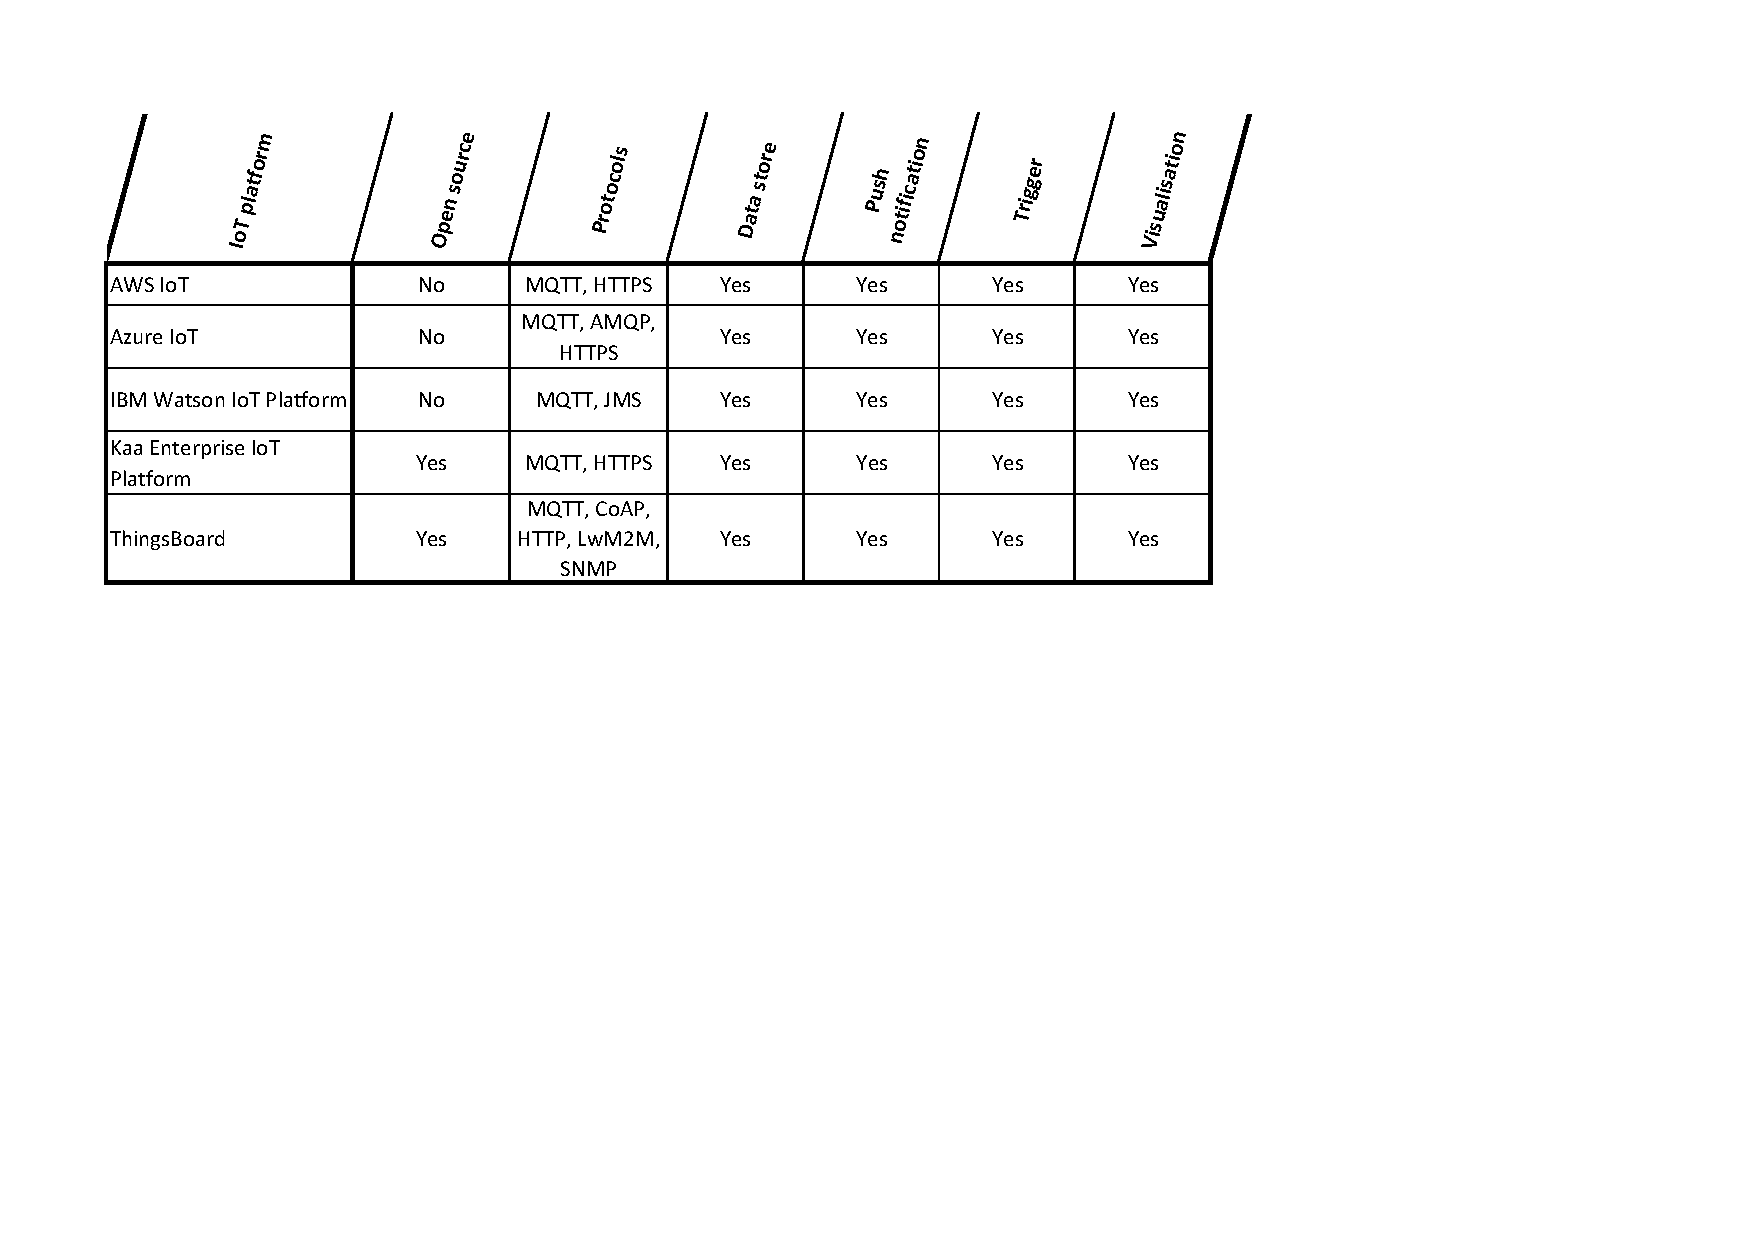
\includegraphics[width=1\columnwidth]{analysis/cloud_providers.pdf}
    \captionof{figure}{Comparison of \acrshort{iot} \gls{cloud} platform providers (sources from providers)}
    \label{fig:cloud_providers}
    \endgroup
\end{center}
Looking at the back end of platforms, they would have an advantage in using containerisation over traditional virtual machines \cite{container_cloud_platform}. It is seen as a lightweight virtualisation solution, with greater flexibility. In addition, containers are proving particularly suitable for solving the platform issues commonly associated with \acrshort{paas} services in the \gls{cloud}. This includes aspects such as application packaging and coordination \cite{container_cloud_platform}. Docker is the most popular container solution \cite{docker}. As for container orchestration, there's Kubernetes, an open source system \cite{k8s}.


% ------------------------------------------------------------------------------
\section{\texorpdfstring{\Gls{cloud}}{} infrastructure tools}
\label{subsec:iac_tools}

% -- Your text goes here --
When you want to host applications in the \gls{cloud}, you need to deploy a \gls{cloud_infrastructure}. It is perfectly possible to build the infrastructure manually. All you have to do is visit a \gls{cloud} provider's web page and select the resources you need from the services on offer. However, this infrastructure could be deployed several times. Fortunately, there are tools that can automatically deploy \glspl{cloud_infrastructure}, called \acrfull{iac}. The automatic deployment of \glspl{cloud_infrastructure} corresponds to \gls{provisioning}. These tools use templates containing a description of the infrastructure based on executable code or a configuration file. They save time on deployment and ensure that the implementation policy behind the infrastructure is always the same (security, rules, etc.). In addition to \gls{provisioning}, \acrshort{iac} tools are capable of updating and deleting an infrastructure. There are universal \gls{provisioning} tools for different \gls{cloud} providers and there are integrated tools for each provider. \cite{iac_tools}

\subsection{Integrated \acrshort{iac} tools}
Having mentioned the \gls{aws} and Microsoft Azure providers in section \ref{subsec:cloud_providers}, each of them has its own \acrshort{iac} tool reserved for use with its platform. Google \Gls{cloud} is not mentioned in this section due to the cessation of \acrshort{iot} activities.

At \gls{aws}, there are two \acrshort{iac} tools. \gls{aws} CloudFormation \cite{aws_cloudformation} is the first. \gls{aws} \acrfull{cdk} \cite{aws_cdk} is the second for defining and building infrastructure in the \gls{aws} \gls{cloud} environment. \gls{aws} \acrshort{cdk} gives users the flexibility to define infrastructure in distinct programming languages in the form of an application, with imperative syntax. It uses \gls{aws} CloudFormation as the deployment engine and allows users to define the infrastructure using programming idioms to model the system design. The \acrshort{cdk} application deployment process includes the construction of the defined elements, preparation, validation and synthesis of the deployment artefacts. The \acrshort{cdk} application is then transferred to the \gls{aws} CloudFormation service for real deployment. An overview of the deployment is shown in figure \ref{fig:aws_iac}. The basic elements of \acrshort{cdk} applications are called "constructs", and they represent \gls{cloud} components containing services. Constructs can be nested to create a hierarchy of dependencies called a "construct tree". Ultimately, this hierarchy defines how constructs are synthesized into resources in the final \gls{aws} CloudFormation model. In a \acrshort{cdk} application, it is possible to define several stacks. These are unique deployment units, each containing a hierarchy of constructs. \cite{iac_tools}
\begin{center}
    \begingroup
    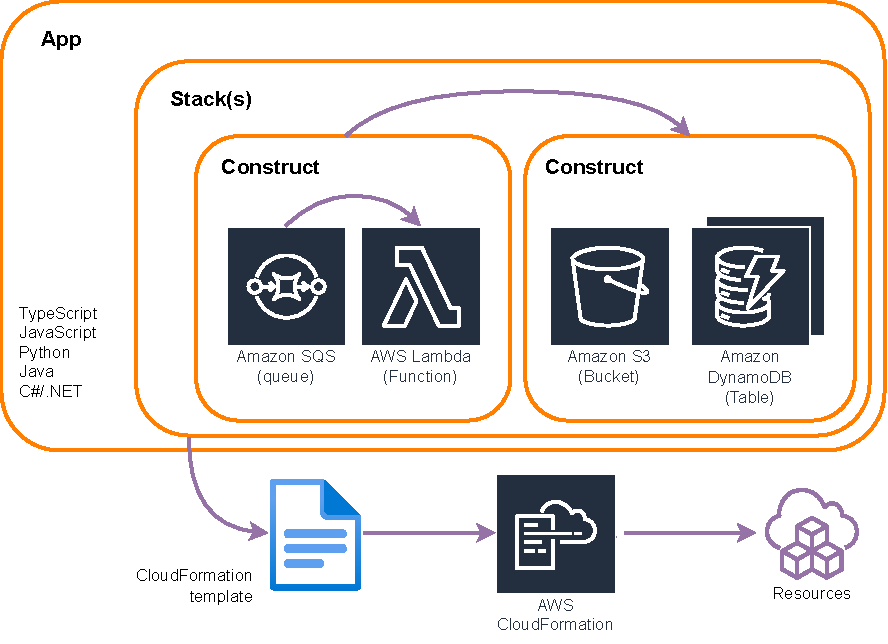
\includegraphics[width=1\columnwidth]{analysis/aws_iac.pdf}
    \captionof{figure}{Overview of \gls{aws} \acrshort{cdk} \cite{aws_cdk} deployment \cite{aws_cdk}}
    \label{fig:aws_iac}
    \endgroup
\end{center}

Microsoft Azure offers the \acrfull{a_arm} deployment and management service \cite{azure_arm}. All actions performed on resources by the user go through the \acrshort{a_arm} manager. It authenticates and authorises them. At the deployment level, there are \acrshort{a_arm} models, which are \acrshort{json} files defining the infrastructure and configuration of a \gls{cloud} environment. \acrshort{json} uses declarative syntax. Before deployment, the \acrshort{a_arm} \acrshort{api} checks the models for possible errors, guaranteeing successful deployment. \acrshort{a_arm} models ensure an identical architecture for deployments in different environments, such as development, testing and production, for example. The fewer dependencies there are, the faster \acrshort{a_arm} can deploy infrastructure resources in parallel. \acrshort{a_arm} models can be segmented into modular files for easy reuse. A group of resources deployed in the Azure platform can be extracted in the form of an \acrshort{a_arm} model. \cite{iac_tools}

\subsection{Universal \acrshort{iac} tools}
There are several \acrshort{iac} tools compatible with different \gls{cloud} platforms such as \gls{aws}, Microsoft Azure, and many others. The \nameref{subsec:56k.cloud} company mainly uses Terraform \cite{terraform} and Pulumi \cite{pulumi}.

Terraform is a tool created in 2014 by HashiCorp, written in the Go programming language \cite{terraform_github}. It mainly provisions \acrlong{iaas}, but can also deploy \acrlong{paas} and \acrlong{saas}. Terraform works using two inputs: configuration and state. The desired resources in the \gls{cloud_infrastructure} are described in a configuration file. This file works with the Terraform language using declarative syntax. The state corresponds to the current state of the infrastructure, or in other words the stack. The state is managed by the Terraform \acrshort{api} and is stored locally by default. The deployment engine compares the desired infrastructure with the current state and determines which resources need to be created, updated or deleted. Terraform uses provider plugins to interact with \gls{cloud} providers. It offers five basic commands for different stages: "init", "validate", "plan", "apply" and "destroy", enabling the infrastructure to be managed efficiently and easily \cite{terraform}. The "init" command prepares the project directory. The "validate" command checks that the configuration is valid. The "plan" command displays the changes required by the current configuration. The "apply" command creates or updates the \gls{cloud_infrastructure}. Finally, the "destroy" command destroys the \gls{cloud_infrastructure}. An overview of the deployment can be seen in figure \ref{fig:terraform_iac}. \cite{iac_tools}
\begin{center}
    \begingroup
    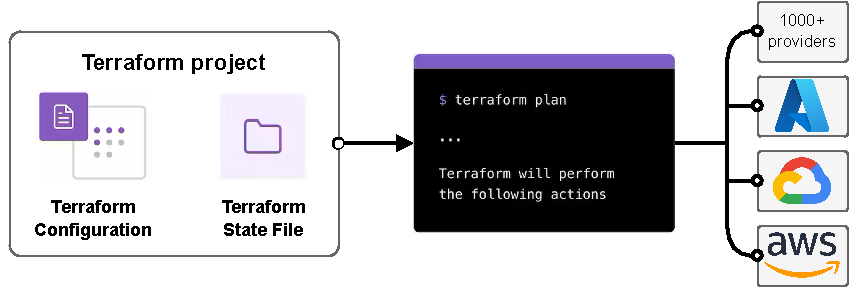
\includegraphics[width=1\columnwidth]{analysis/terraform_iac.pdf}
    \captionof{figure}{Overview of Terraform deployment \cite{terraform}}
    \label{fig:terraform_iac}
    \endgroup
\end{center}

Pulumi is an \acrshort{iac} tool similar to Terraform, but open source. It is written in the Go language \cite{pulumi_github}. Version 1.0 of Pulumi was released in 2019. This tool can be used with several programming languages, such as TypeScript, JavaScript, Python, Go and .NET. It therefore offers developers the possibility of creating \glspl{cloud_infrastructure} using standard technologies, unlike Terraform. Deployment follows the Terraform model, where a Pulumi application is run to schedule the desired resources in the \gls{cloud_infrastructure}. The deployment engine compares these desired resources with the current state of the stack and determines the necessary actions. The state of the last infrastructure deployment is saved in the Pulumi \Gls{cloud} platform by default. With the Pulumi tool, we're talking about applications, because it uses imperative syntax. Applications describe how the \gls{cloud_infrastructure} should be composed by allocating resource objects whose properties correspond to the desired state. Resources are deployed in parallel if possible, but some resources have dependencies between them. Deployment is managed by the Pulumi \acrshort{cli}. An overview of deployment is shown in figure \ref{fig:pulumi_iac}. \cite{iac_tools}
\begin{center}
    \begingroup
    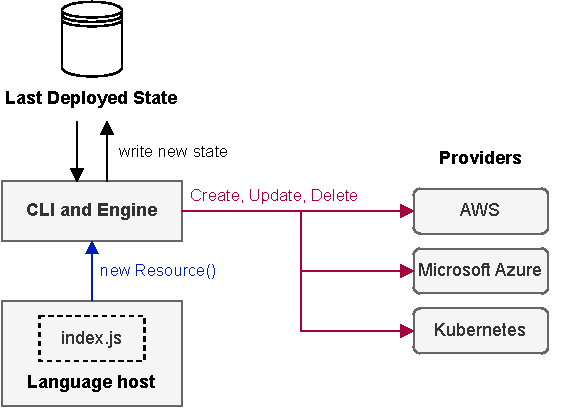
\includegraphics[width=.8\columnwidth]{analysis/pulumi_iac.pdf}
    \captionof{figure}{Overview of Pulumi deployment \cite{pulumi}}
    \label{fig:pulumi_iac}
    \endgroup
\end{center}

\subsection{Comparison}
Without even using the \acrshort{iac} tools, it is possible to identify a few differences. The tools integrated with the \gls{cloud} providers cannot be used outside their platform. The other two tools, Terraform and Pulumi, can be provisioned by different providers. One notable point concerns the syntax. Terraform and Microsoft Azure use descriptive syntaxes. These limit the variety of programming languages. Terraform has its own language which you need to familiarise yourself with the first time. \gls{aws} and Pulumi use imperative syntax, which leaves the choice of programming languages open.

Focusing on the practical side, other disparities were noted. These stem from a project that was carried out with the aim of comparing the different \acrshort{iac} tools mentioned in this section \ref{subsec:iac_tools} \cite{iac_tools}. Terraform has several advantages, including clear documentation, an understandable configuration language, real-time execution plans and the ability to structure the infrastructure by dividing scripts into separate files. Because \gls{cloud} providers have different services, it is impossible to reuse the same code with each of them. It is possible to maintain the overall architecture of the infrastructure if the entities are clearly separated in the scripts. On the Pulumi side, resources can be separated into classes or functions. Common code between providers is therefore limited to abstractions of classes and functions. Pulumi has developed a tool capable of converting Terraform scripts into Pulumi scripts. It differs from Terraform by using Pulumi \Gls{cloud} for infrastructure state management by default instead of a self-managed \acrshort{api}. This is an advantage of not needing to store state files locally and manage them. Terraform and Pulumi generally use \acrshort{api}s from \gls{cloud} providers to create resources. One case stands out with Pulumi, when it works with \gls{aws}, it uses the \gls{aws} \acrshort{sdk} service directly, which will create the resources. Concerning the \acrlong{a_arm} tool, it is less efficient than \gls{aws} \acrshort{cdk} because of the complexity of the configuration files. \gls{aws} \acrshort{cdk} offers better readability by being able to divide up the code as required. Despite all this, it should be noted that these four \acrshort{iac} tools were able to provision the project in question. \cite{iac_tools}


% ------------------------------------------------------------------------------
\section{\texorpdfstring{\gls{arm}}{} SystemReady}
\label{sec:arm_systemready}

% -- Your text goes here --
Manufacturer \gls{arm} has decided to introduce a certification programme called SystemReady \cite{systemready_program}. In 2020, as part of \gls{arm}'s Cassini project, SystemReady was introduced to address the compatibility concerns of users planning to move from x86 architectures to systems based on \gls{arm}'s processors \cite{systemready_approval}. \gls{arm} defines its programme as follows:
\begin{quote}
    \textit{\nameref{sec:arm_systemready} is a compliance certification program based on a set of hardware and firmware standards: \acrfull{bsa} and \acrfull{bbr} specifications, plus a selection of supplements. This ensures that subsequent layers of software also ‘just work’. The compliance certification program tests and certifies that systems meet the SystemReady standards, giving confidence that operating systems \acrshort{os} and subsequent layers of software just work. \cite{systemready_program}}\\
\end{quote}

The \gls{arm} \acrshort{bsa} specification establishes a hardware basis for system software, including \acrshort{os}s, hypervisors and firmware, based on the 64-bit \gls{arm} architecture. This specification ensures that users can install, boot and run generic \acrshort{os}s and hypervisors \cite{bsa_standard}. The \acrshort{bbr} specification complements \acrshort{bsa} by defining the basic firmware requirements necessary to support any \acrshort{os} or hypervisor compatible with the \acrshort{bsa} specification \cite{bbr_standard}.

A number of advantages were mentioned in relation to the program \cite{systemready_program}:
\begin{itemize}
    \item[—] Compliance allows \acrshort{os}s and workloads to operate seamlessly on different \gls{arm} platforms.
    \item[—] Standardisation of a range of different devices and systems provides a stable basis and a choice of systems for all sectors.
    \item[—] Compliance with standards inspires confidence in software compatibility, so developers can concentrate on innovation and adding value to their products.
    \item[—] Compliance simplifies and accelerates time-to-market for partners.
    \item[—] Compliance makes it easy to identify \gls{arm}-based devices thanks to the "SystemReady certified" stamp.
    \item[—] Compliance makes it easy to deploy and maintain standard firmware interfaces, reducing maintenance costs.
    \item[—] Compliance reduces the costs associated with adopting a new platform by eliminating custom firmware engineering.
\end{itemize}

\subsection{SystemReady certifications}
To be able to adapt to different types of devices and markets, \gls{arm} has introduced four certifications. The first is SystemReady SR. It ensures the smooth operation of servers or workstations on a \gls{arm} chip. It is specially designed for Windows, Linux, VMware and \acrfull{bsd} environments. It targets generic out-of-the-box \acrshort{os}s and also supports legacy \acrshort{os}s on new devices. \cite{systemready_program}

SystemReady ES is designed to meet the needs of Windows, Linux, VMware and \acrshort{bsd} ecosystems based on \gls{arm} embedded systems. It also targets generic out-of-the-box \acrshort{os}s and supports legacy \acrshort{os}s on new devices. \cite{systemready_program}

SystemReady IR ensures that Linux and \acrshort{bsd} work perfectly on \gls{arm} embedded systems. It is ideally suited to the \acrshort{iot} sector. It mainly targets the Linux environment, but also custom images (Yocto, OpenWRT, buildroot) and pre-built images (Debian, Fedora, SUSE). \cite{systemready_program}

SystemReady LS specifies the correct operation of Linux \acrshort{os}s on \gls{arm} chips designed for servers. This certificate is mainly for hyperscalers. Hyperscalers are large \gls{cloud} service providers. \cite{systemready_program}

At present, a multitude of hardware design companies are partnering with \gls{arm} to follow the SystemReady standards. Several embedded systems are already certified and on the market.
% ------------------------------------------------------------------------------
% In the design section a general overview about the system to be implemented is
% shown. All the hardware, software, communications and other topics are
% evaluated and selected.
% ------------------------------------------------------------------------------

\opt{never}{\addbibresource{03-tail/bibliography.bib}} % to make citation found in most IDE

\chapter{Design}
\label{chap:design}

% -- Your text goes here --
The design shows an overview of the different parts of the reference architecture. It describes the idea behind the structure of the \gls{cloud_infrastructure} with the integration of several embedded systems. The general operation of each of the applications included in this architecture is also described.

\minitoc
\newpage

% ------------------------------------------------------------------------------
\section{Reference architecture}

% -- Your text goes here --
The reference architecture is divided into two parts: the first concerns embedded systems based on \gls{arm} architectures and certified \nameref{sec:arm_systemready} with a Linux operating system, while the second relates to the \gls{cloud} and is hosted by the \gls{aws} provider. An overview is clearly shown in figure \ref{fig:RefArch_Overview}.
\begin{center}
    \begingroup
    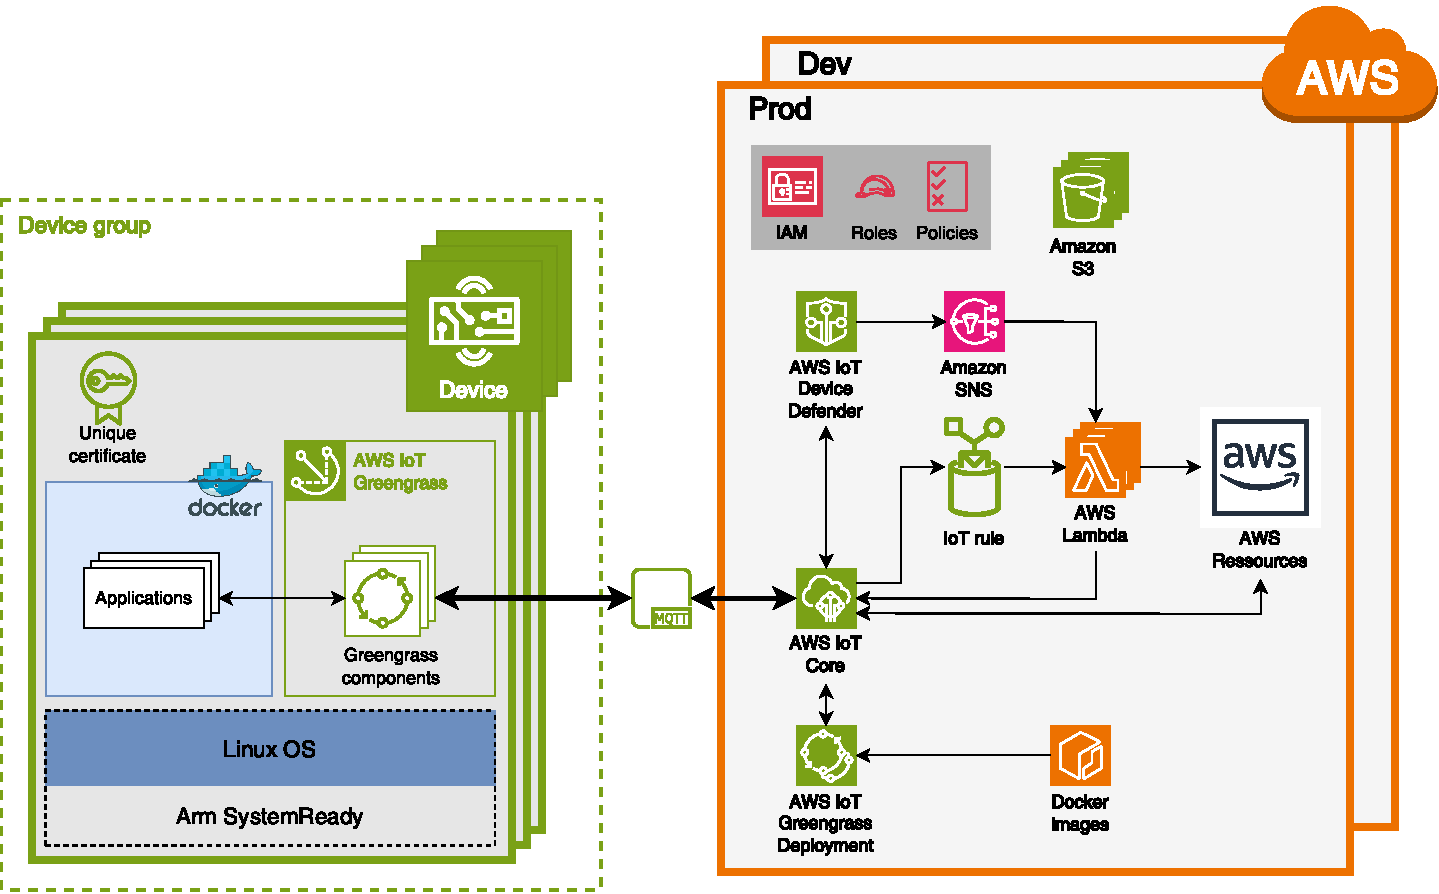
\includegraphics[width=1\columnwidth]{design/RefArch_Overview.pdf}
    \captionof{figure}{Reference architecture overview}
    \label{fig:RefArch_Overview}
    \endgroup
\end{center}

\subsection{\Gls{cloud_infrastructure}}
In the \gls{cloud}, two distinct infrastructures are presented. The first infrastructure is dedicated to development, enabling all kinds of operations to be tested. The second infrastructure is the production infrastructure, encompassing the final product intended for customers. Each infrastructure uses different \gls{aws} services.

The central service managing the \acrshort{iot} is \gls{aws} \acrshort{iot} Core, which exchanges data with all connected devices. Its preferred communication protocol is \acrshort{mqtt}. Provisioned devices are registered in a specific group within this service. Only authorised devices are provisioned. \gls{aws} \acrshort{iot} Greengrass Deployment handles the deployment of new Greengrass components or updates to a group of devices. A component, in the context of \gls{aws} \acrshort{iot} Greengrass, is a unit of deployment and execution that encapsulates code, dependencies and resources, making it easy to deploy, manage and update \acrshort{iot} applications. In this architecture, Docker components are used, encapsulating Docker containers to offer greater flexibility in software deployment. Docker images are stored in the Amazon \acrfull{ecr}. Another service, \gls{aws} \acrshort{iot} Device Defender, checks daily whether a certificate is about to expire, as each device has a unique certificate enabling a secure connection. If a certificate expires within 30 days, it is replaced by a new one. Other Lambda functions, triggered by rules, can enrich the architecture, as can other \gls{aws} resources, depending on the needs of each developer. Storage spaces such as Amazon S3 are used to save the state of the infrastructure, configuration files and \acrshort{os} images. The configuration files contain a list of the serial numbers of all the \acrshort{iot} devices authorised to be provisioned. If a device is not listed and attempts to be provisioned, access will be denied. If a device is already provisioned and its serial number is removed from the list, its access will be withdrawn and it will be deleted from the \gls{cloud}. The IAM service is there to assign roles and policies, limiting authorised actions on resources to the strict minimum.

\subsection{Embedded systems integration}
Embedded systems must be based on \gls{arm} architecture and be \nameref{sec:arm_systemready} certified. The devices are flashed with a custom Linux \acrshort{os} image. On first boot, two software programs are installed : Docker Engine for running Docker containers, and \gls{aws} \acrshort{iot} Greengrass Core for \gls{provisioning}, communicating with \gls{aws} \acrshort{iot} Core and managing Greengrass components. This software provisions the device by exchanging the claim certificate with a unique certificate, securing the connection of the device, which is then registered in the device group. Deployment of Greengrass components from the \gls{cloud} to devices is automated when a new device is associated or a new version of a component becomes available. Applications are contained in Docker containers to ensure optimum portability.


% ------------------------------------------------------------------------------
\section{\texorpdfstring{\acrshort{ci}/\acrshort{cd}}{} pipeline}

% -- Your text goes here --
The pipeline is made up of several workflows, each dedicated to a specific function. An overview of the various stages in the pipeline is shown in figure \ref{fig:CICD_Pipeline_Overview}. The pipeline uses \acrshort{ci}/\acrshort{cd} methods to automate the deployment of the \gls{cloud_infrastructure}, as well as preparing for the integration of embedded systems.
\begin{center}
    \begingroup
    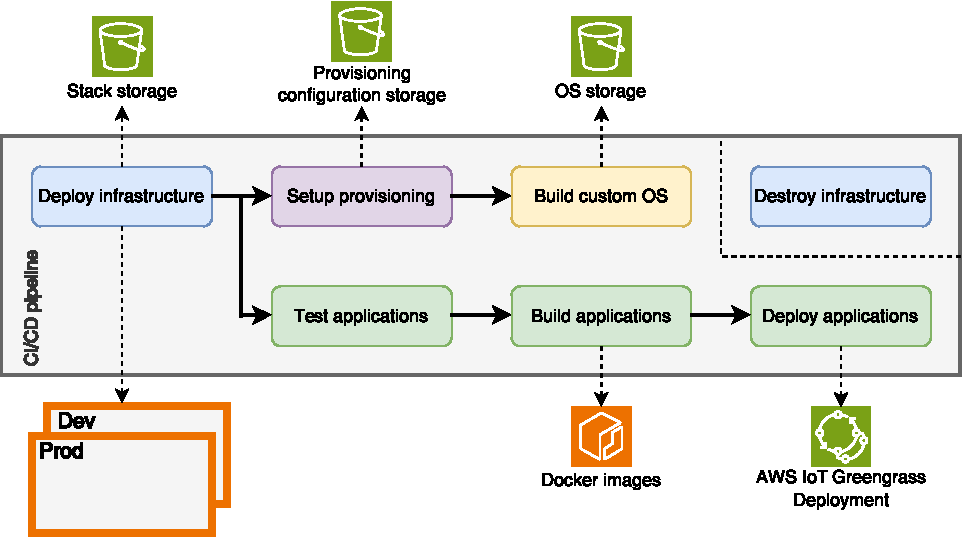
\includegraphics[width=1\columnwidth]{design/CICD_Pipeline_Overview.pdf}
    \captionof{figure}{\acrshort{ci}/\acrshort{cd} workflows overview}
    \label{fig:CICD_Pipeline_Overview}
    \endgroup
\end{center}
The first job is to deploy the \gls{aws} \gls{cloud_infrastructure} (\textit{Deploy infrastructure}). It can enable the deployment of development or production infrastructure. Since it uses a tool called \acrshort{iac}, the state of the infrastructure must be stored. This flow also enables resources to be updated.

If the entire infrastructure is deployed without error, the provisioning configuration workflow (\textit{Setup \gls{provisioning}}) takes care of preparing configuration files for \gls{provisioning} in a storage space. It also manages device control. It checks the list of authorised devices to identify whether a previously provisioned device has been removed from the list. If so, it will be removed from the \gls{cloud}. It may also be the case that authorised devices have already been provisioned and need to be connected to the new infrastructure. This operation is also checked and carried out.

If the previous step has been successful, the next step (\textit{Build custom \acrshort{os}}) is to prepare and create the \acrshort{os} image with all the files and scripts needed to automatically provision the devices when they start up for the first time. The image must be saved in a storage space that allows it to be downloaded for flashing the devices' SD cards.

In parallel with the previous two workflows, the application workflows are launched. The first (\textit{Test applications}) performs various tests on the applications. It includes security and unit tests.

If the tests have not failed, the next job (\textit{Build applications}) is to build the Greengrass components from the applications. A Docker image is first created for each of the applications, coded in a freely chosen programming language. These images are then linked to their respective components. Finally, the components must be saved in the \gls{aws} \acrshort{iot} Greengrass service to be ready for deployment.

The last flow (\textit{Deploy applications}) takes care of deploying applications to the device group. It uses the Greengrass Deployment service.

After all these tasks, there is still the infrastructure dismantling workflow (\textit{Destroy infrastructure}). It is independent and can be launched manually. It is available in the event that a problem occurs and the infrastructure needs to be redeployed.

% ------------------------------------------------------------------------------
\section{Applications}

% -- Your text goes here --
Several applications have been developed. Some are essential to the reference architecture, while others are demonstration applications. An overview of these is shown in figure \ref{fig:apps_overview}.
\begin{center}
    \begingroup
    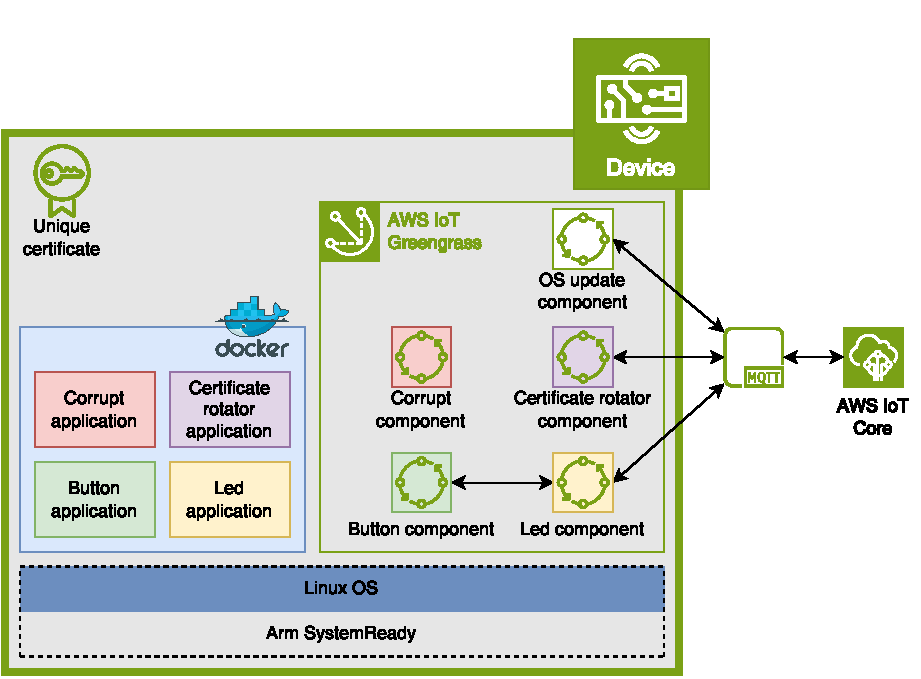
\includegraphics[width=1\columnwidth]{design/apps_overview.pdf}
    \captionof{figure}{Applications overview}
    \label{fig:apps_overview}
    \endgroup
\end{center}

\subsection{\acrshort{os} update}
The application used to update \acrlong{os} features is essential to the reference architecture. Keeping Linux up to date is essential for security, stability, performance and compatibility. Security updates correct vulnerabilities, minimising the risk of exploitation by malicious software. Bug fixes and performance optimisations improve system stability and efficiency. Updating also ensures compliance with security requirements and adaptation to new features and standards. By keeping a Linux \acrshort{os} up to date, users can ensure that their system runs at optimum performance while keeping pace with technological developments and industry requirements.

This application does not run in a Docker container, but directly in the Greengrass component. The operation of the application must be kept simple. An activity diagram in figure \ref{fig:activity_diagram_OS_update} shows this.
\begin{center}
    \begingroup
    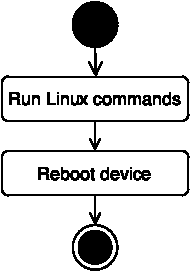
\includegraphics[width=.2\columnwidth]{design/activity_diagram_OS_update.pdf}
    \captionof{figure}{\acrshort{os} update application activity diagram}
    \label{fig:activity_diagram_OS_update}
    \endgroup
\end{center}
When the component starts up the first time the device is launched or after it has been updated, it will execute the Linux commands that have been written. To enable a complete update, the device will restart automatically. The component executes the Linux commands only once for each new version of the component.

\subsection{Certificate rotation}
On embedded systems communicating with \gls{aws}, unique certificates are used to establish secure connections via the protocols. Certificates have expiry dates for security reasons. The use of certificates with an expiry date makes it possible to limit the time during which a certificate is considered valid. This helps to reduce the risks associated with compromised private keys and ensures that certificates are regularly renewed, incorporating the latest security standards. It is therefore crucial to update certificates on embedded systems before their expiry date. If a certificate expires, secure connections with \gls{cloud} services may be interrupted, leading to communication problems. To avoid this, this application must allow certificates to be managed automatically. It works with the \gls{aws} \acrshort{iot} Device Defender service, which alerts the application when it is time to change a certificate.

This application runs in a Docker container. An activity diagram illustrates its behaviour in figure \ref{fig:activity_diagram_certificate_rotator}.
\begin{center}
    \begingroup
    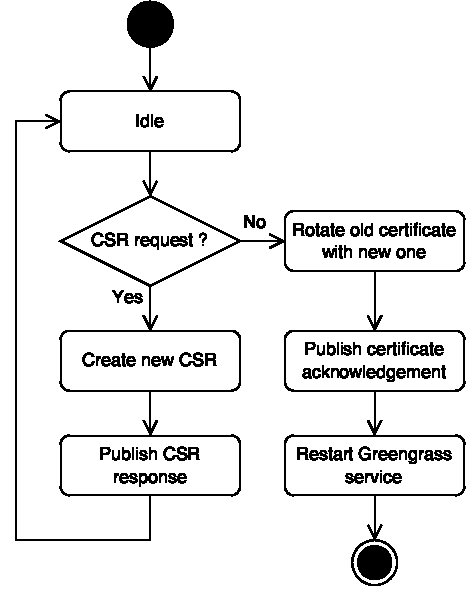
\includegraphics[width=.5\columnwidth]{design/activity_diagram_certificate_rotator.pdf}
    \captionof{figure}{Certificate rotator application activity diagram}
    \label{fig:activity_diagram_certificate_rotator}
    \endgroup
\end{center}
The general idea is that it is alerted by the \acrshort{iot} Device Defender service when a certificate change is required. The application then creates a new private key and makes a certificate creation request (\acrfull{csr}) to the Amazon root certificate authority. A signed certificate is returned. This will replace the old certificate and the old private key with the new one. In order for the \gls{aws} \acrshort{iot} Greengrass Core service to take the new certificate into account during future communications, this service must be restarted on the device. An overview of the certificate rotation is shown in figure \ref{fig:CertificateRotation_Overview}. It shows the links between the \gls{aws} services and the application on the \acrshort{iot} device.
\begin{center}
    \begingroup
    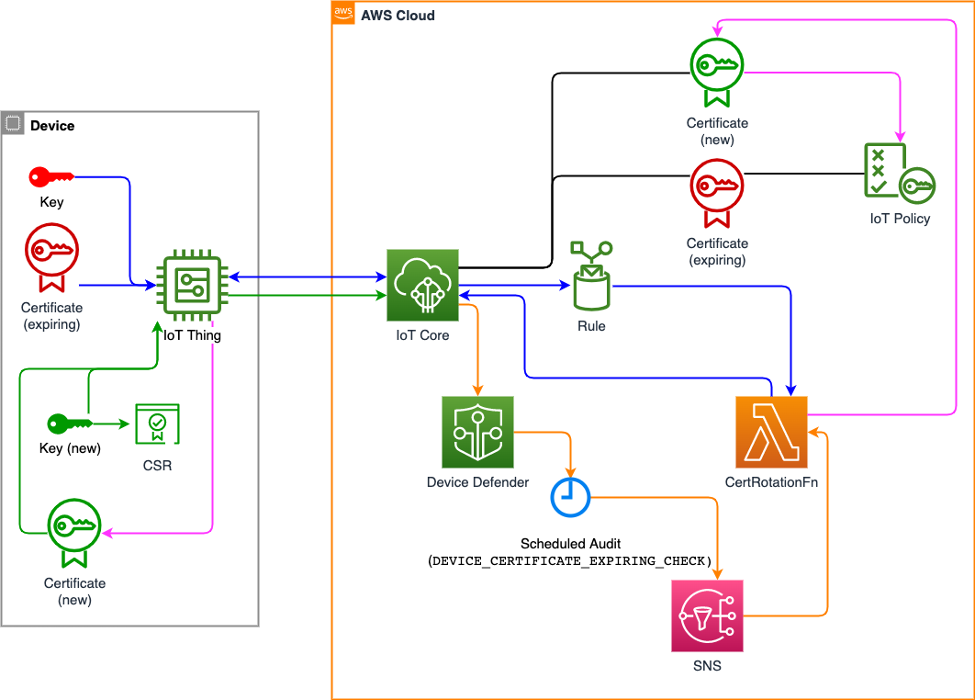
\includegraphics[width=1\columnwidth]{design/CertificateRotation_Overview.png}
    \captionof{figure}{Certificate rotation overview \cite{aws_iot_certificate_rotator}}
    \label{fig:CertificateRotation_Overview}
    \endgroup
\end{center}

\subsection{Led application}
\label{subsec:led_app}
This application is not essential to the reference architecture. It is used as a demonstration for \acrshort{mqtt} communication with \gls{aws} \acrshort{iot}. It is an application in a Docker container that blinks an led on an embedded system. The blinking frequency can be adjusted from an application associated with \gls{aws} \acrshort{iot} using the \acrshort{mqtt} protocol. Blinking can also be enabled or disabled from the \hyperref[subsec:button_app]{button application}. Two pieces of data, the blink frequency and the blink state, are transmitted to \gls{aws} \acrshort{iot} so that they can be viewed on an interface. This is shown in figure \ref{fig:use_case_led_button_apps}.
\begin{center}
    \begingroup
    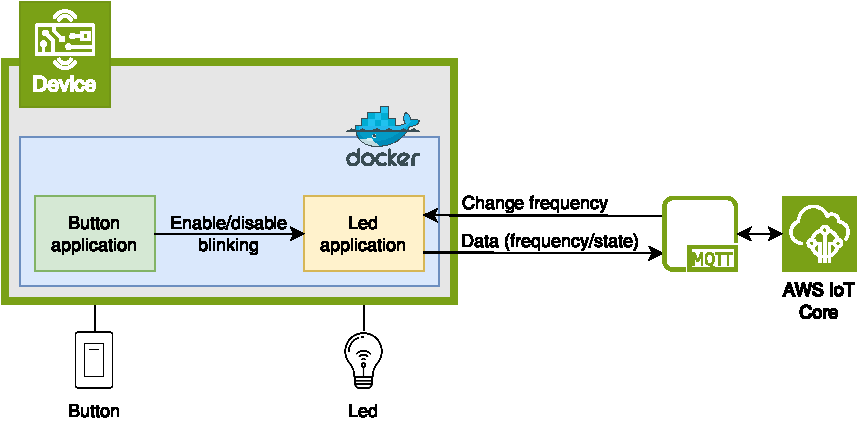
\includegraphics[width=1\columnwidth]{design/use_case_led_button_apps.pdf}
    \captionof{figure}{Led and button applications use case}
    \label{fig:use_case_led_button_apps}
    \endgroup
\end{center}

\subsection{Button application}
\label{subsec:button_app}
This application is connected to the \hyperref[subsec:led_app]{led application} while retaining its independence. It is designed as a demonstration of local \acrshort{mqtt} communication. Also running in a Docker container, it simply interacts with the \hyperref[subsec:led_app]{led application} to activate or deactivate the blinking of the led. The user presses a button built into the device to reverse the blinking state. A high-level view is shown in figure \ref{fig:use_case_led_button_apps}.

\subsection{Corrupt application}
A corrupted application is also developed to examine the behaviour of the device with \gls{aws} services. The approach is to run a simple Docker application by deliberately providing an incorrect environment for launching the container.
% ------------------------------------------------------------------------------
% The implemtations shows specifically how your research was conducted.
% All the impementation details and practical tests can be listed.
% ------------------------------------------------------------------------------

\opt{never}{\addbibresource{03-tail/bibliography.bib}} % to make citation found in most IDE

\chapter{Implementation}
\label{chap:implementation}

% -- Your text goes here --
The implementation sets out the concrete realisation of the reference architecture, detailing the tools used to automate the deployment of the \gls{cloud_infrastructure} and the integration of the embedded systems. Particular attention is paid to the in-depth description of the automated pipeline. The various applications that accompany this architecture are also highlighted.

\minitoc
\newpage

% ------------------------------------------------------------------------------
\section{Reference architecture}

% -- Your text goes here --
\subsection{\Gls{cloud_infrastructure}}
An \acrfull{iac} tool was selected to orchestrate the efficient deployment of the \gls{cloud_infrastructure} on \gls{aws}, and Pulumi was chosen because of its choice of programming language, in this case Python. The use of the same programming language for the implementation of applications and the description of \gls{aws} resources provides consistency within the project.

Integrating Pulumi is simple. The resources required are described in Python files. The deployment is managed by the Pulumi \acrshort{cli}, which records the state of the infrastructure in an Amazon S3 compartment. This compartment is located in the same \gls{aws} account as the infrastructure, using Amazon S3 to store the state rather than the default Pulumi \Gls{cloud} platform, thus eliminating external dependencies. Figure \ref{fig:pulumi_overview} shows an overview of this part of the implementation.
\begin{center}
    \begingroup
    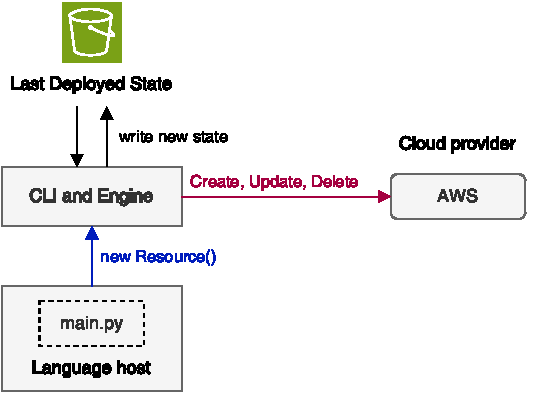
\includegraphics[width=.7\columnwidth]{implementation/pulumi_overview.pdf}
    \captionof{figure}{Overview of Pulumi's integration into the reference architecture}
    \label{fig:pulumi_overview}
    \endgroup
\end{center}
This \gls{cloud_infrastructure} part is implemented in a specific folder as follows :
\begin{center}
    \usemintedstyle{pastie}
    \begin{minted}
    [
    fontsize=\scriptsize
    ]{text}
    cloud-infrastructure
        ├── Pulumi.yaml
        ├── Pulumi.dev.yaml
        ├── Pulumi.prod.yaml
        ├── main.py
        ├── iam.py
        └── requirements.txt
    \end{minted}
\end{center}
The main configuration file for the Pulumi tool, \textit{Pulumi.yaml}, includes crucial information such as the name of the stack and the programming language used, in this case Python.

This implementation aims to facilitate the deployment of two distinct infrastructures, namely the development environment and the production environment. Therefore, two additional configuration files, \textit{Pulumi.dev.yaml} and \textit{Pulumi.prod.yaml}, are present to differentiate these two environments. \textit{Pulumi.dev.yaml} contains parameters such as the \gls{aws} development account ID and the deployment region, while \textit{Pulumi.prod.yaml} includes the same parameters with production-specific values. The identifiers of the \gls{aws} accounts must be different.

The Python files \textit{main.py} and \textit{iam.py} detail the description of the resources to be deployed. \textit{iam.py} focuses on IAM roles and policies, while \textit{main.py} mainly covers resources related to \acrshort{iot} and other resources.

Finally, the \textit{requirements.txt} file lists the Pulumi libraries to be installed, including the main Pulumi library, which is essential for all \acrshort{iac} projects.

In terms of the Pulumi libraries used, \gls{aws} Native, a new preview, uses the \gls{aws} \Gls{cloud} Control API to manage and provision \gls{aws} resources, generally aligning with the latest \gls{aws} features as they are released. The resources available in this library are based on those defined in the \gls{aws} CloudFormation registry. In addition, \gls{aws} Classic is another library that is used to fill in resources that are not yet available in \gls{aws} Native. This library uses the \gls{aws} SDK to manage and provision these resources.


\subsection{Embedded systems integration}
\subsubsection{\gls{aws} \acrshort{iot} Greengrass}
Integrating embedded systems with the \gls{aws} ecosystem is crucial to reaping the full benefits of \hyperref[subsec:cloudcomputing]{cloud computing}. To this end, \gls{aws} \acrshort{iot} Greengrass was chosen, a powerful solution that facilitates the execution of local processing on \acrshort{iot} devices, while enabling seamless interaction with \gls{aws} \gls{cloud} services. \gls{aws} defined this solution as follows :
\begin{quote}
    \textit{\gls{aws} \acrshort{iot} Greengrass is an open source \acrfull{iot} edge runtime and \gls{cloud} service that helps you build, deploy and manage \acrshort{iot} applications on your devices. You can use \gls{aws} \acrshort{iot} Greengrass to build software that enables your devices to act locally on the data that they generate, run predictions based on machine learning models, and filter and aggregate device data. \gls{aws} \acrshort{iot} Greengrass enables your devices to collect and analyze data closer to where that data is generated, react autonomously to local events, and communicate securely with other devices on the local network. Greengrass devices can also communicate securely with \gls{aws} \acrshort{iot} Core and export \acrshort{iot} data to the \gls{aws} Cloud. You can use \gls{aws} \acrshort{iot} Greengrass to build edge applications using pre-built software modules, called components, that can connect your edge devices to \gls{aws} services or third-party services. You can also use \gls{aws} \acrshort{iot} Greengrass to package and run your software using Lambda functions, Docker containers, native operating system processes, or custom runtimes of your choice. \cite{aws_iot_greengrass}}\\
\end{quote}
In this implementation, \gls{aws} \acrshort{iot} Greengrass Core software is deployed on embedded systems, acting as an intelligent hub that manages interactions with the \gls{aws} \gls{cloud}. It adapts perfectly to Linux OS. Greengrass components, encapsulating the necessary code, dependencies and resources, are then deployed automatically using mechanisms such as \gls{aws} \acrshort{iot} Greengrass Deployment.

A component must be installed. \textit{Greengrass nucleus} (aws.greengrass.Nucleus) is a mandatory component and the minimum requirement for running \gls{aws} \acrshort{iot} Greengrass Core software on a device. It is configurable to customize and update the \gls{aws} \acrshort{iot} Greengrass Core software \acrlong{ota}.

\subsubsection{Communication}
In this project, components running on an embedded system use the \gls{aws} \acrshort{iot} Greengrass Core \acrfull{ipc} library, available in the \gls{aws} \acrshort{iot} Device SDK, to exchange data with the \gls{aws} \acrshort{iot} Greengrass nucleus and other Greengrass components. The \acrshort{ipc} interface supports the \acrlong{mqtt} communication protocol. \acrshort{mqtt} offers lightweight, asynchronous communication.

Publish/subscribe messaging allows messages to be sent and received in topics. Components can publish messages in topics to communicate with other components, and those who have subscribed to the topic can act on messages received. In this case, the communication is local to the \acrshort{iot} device.

The \acrshort{ipc} interface also facilitates the sending and receiving of \acrshort{mqtt} messages between \gls{aws} \acrshort{iot} Greengrass and \gls{aws} \acrshort{iot} Core. Components can publish messages to \gls{aws} \acrshort{iot} Core and subscribe to topics to react to \acrshort{mqtt} messages from other sources.

\subsubsection{\acrshort{ota} update}
All devices with \gls{aws} \acrshort{iot} Greengrass Core software can obtain \acrshort{ota} updates via \acrshort{mqtt}.

\textbf{\gls{aws} \acrshort{iot} Greengrass Core software update}\\
This functionality is built into the \gls{aws} \acrshort{iot}Greengrass Core software. It is made possible by the \textit{Greengrass nucleus} component and other optional components. The following information is taken from the \gls{aws} documentation \cite{ota_aws_iot}.

A few prerequisites must be met before an update can be carried out. Firstly, the Greengrass device must be connected to the \gls{cloud} \gls{aws} in order to receive the deployment. It must be properly configured with certificates and authentication keys to interact with both the \gls{aws} \acrshort{iot} Core and \gls{aws} \acrshort{iot} Greengrass. Finally, the \gls{aws} \acrshort{iot} Greengrass Core software must be configured and run as a system service.

There are a few things to bear in mind when upgrading. The Greengrass nucleus stops. This stops all the other components present. When the nucleus component is shut down, the device's connection to \gls{aws} is lost.

The following table summarises the behaviour of Greengrass updates :

\begin{tabularx}{1\textwidth} { 
    | >{\raggedright\arraybackslash}X 
    | >{\raggedright\arraybackslash}X 
    | >{\raggedright\arraybackslash}X | }
    \hline
    \rowcolor{lightgray}
    Action              & Deployment configuration  & Nucleus update behavior \\ \hline
    \multirow{2}{\linewidth}{Add new devices to a thing group targeted by an existing deployment without revising the deployment.}
    & The deployment does not directly include Greengrass nucleus.
    
    The deployment directly includes at least one AWS-provided component, or includes a custom component that depends on an AWS-provided component or on the Greengrass nucleus.
    & On new devices, installs the latest patch version of nucleus that meets all component dependency requirements.

    On existing devices, does not update the installed version of the nucleus. \\ \cline{2-3}
    & The deployment directly includes a specific version of the Greengrass nucleus.
    & On new devices, installs the specified nucleus version.

    On existing devices, does not update the installed version of the nucleus. \\ \hline
    \multirow{2}{\linewidth}{Create a new deployment or revise an existing deployment.}
    & The deployment does not directly include Greengrass nucleus.

    The deployment directly includes at least one AWS-provided component, or includes a custom component that depends on an AWS-provided component or on the Greengrass nucleus.
    & On all targeted devices, installs the latest patch version of the nucleus that meets all component dependency requirements, including on any new devices that you add to the targeted thing group. \\ \cline{2-3} 
    & The deployment directly includes a specific version of the Greengrass nucleus.
    & On all targeted devices, installs the specified nucleus version, including any new devices that you add to the targeted thing group. \\ \hline
\end{tabularx}

In this reference architecture, the version of \textit{Greengrass nucleus} is not specified. However, there is one component provided by \gls{aws} (\textit{aws.greengrass.Cli}) and custom components which depend on several components provided by \gls{aws}.

\textbf{Greengrass components update}\\
For custom or public \gls{aws} components, the \gls{aws} \acrshort{iot} Greengrass Deployment service enables OTA updates.

The prerequisites for an update are the same as for the software update. When an update is deployed, only components with a new version are updated. These components will then be stopped and restarted automatically after being updated. If a deployment error occurs, a rollback is performed and the components resume their course with the old version.

The following table explains two main actions:

\begin{tabularx}{1\textwidth} { 
    | >{\raggedright\arraybackslash}X
    | >{\raggedright\arraybackslash}X | }
    \hline
    \rowcolor{lightgray}
    Action              & Components behaviour \\ \hline
    Add new devices to a group of devices targeted by an existing deployment without modifying the deployment.
    & All the components and dependencies present in the deployment are automatically deployed with their latest version on the new devices.
    
    On existing devices, nothing happens.\\
    \hline
    Create a new version of one or more Greengrass components.
    & Only components with a new version will be deployed on all devices in the group of devices targeted for deployment. \\
    \hline
\end{tabularx}

\subsubsection{Fleet \gls{provisioning}}
With \gls{aws} \acrshort{iot} fleet \gls{provisioning}, it is possible to securely set up \gls{aws} \acrshort{iot} to generate and distribute X.509 device certificates and private keys to each device when they first connect to \gls{aws} \acrshort{iot} \cite{aws_iot_greengrass_fleet}. These client certificates, signed by the Amazon Root Certificate Authority, are provided by \gls{aws} \acrshort{iot}. It is very flexible to define specific device groups, device types and permissions for Greengrass Core devices to be provisioned using fleet \gls{provisioning}. A \gls{provisioning} template is used to describe the \gls{provisioning} process for each device, detailing the device, policy and certificate resources to be created during \gls{provisioning}. This template is created from Pulumi.

\gls{aws} \acrshort{iot} Greengrass offers a dedicated \gls{aws} \acrshort{iot} fleet \gls{provisioning} plugin (\textit{aws.greengrass .FleetProvisioningByClaim}), which facilitates the installation of \gls{aws} \acrshort{iot} Greengrass Core software using the resources created by \gls{aws} \acrshort{iot} fleet \gls{provisioning}. This plugin uses claim-based \gls{provisioning}, where devices use a \gls{provisioning} claim certificate and private key to obtain a unique X.509 device certificate, along with a private key, enabling regular operations. The claim certificate and private key are integrated as soon as the Linux \acrshort{os} image is created, enabling devices to be activated later when they are connected. The same claim certificate and private key can be used for multiple devices.

To deploy \gls{aws} \acrshort{iot} Greengrass Core software with \gls{aws} \acrshort{iot} fleet provisioning, configuration of resources in the \gls{aws} account is required. These resources include a provisioning template, a claim certificate and a token exchange IAM role. Once these elements have been created from Pulumi, apart from the certificate from the \gls{aws} \acrshort{cli}, they can be reused to provision several embedded systems within the same fleet. The token exchange IAM role authorises calls to \gls{aws} services from the \acrshort{iot} device.

In this architecture, devices are registered by their serial number to ensure that each one has a unique name.
% ------------------------------------------------------------------------------
% Your readers must be able to understand at a glance which data set belongs to which research question or hypothesis.
% - Describe your data objectively
% - Use graphs and tables to illustrate your data.
% - Refer to your research question with each result
% - Rank your results in order of importance
% - Confirm or reject your hypotheses
% ------------------------------------------------------------------------------

\opt{never}{\addbibresource{03-tail/bibliography.bib}} % to make citation found in most IDE

\chapter{Validation}
\label{chap:validation}

% -- Your text goes here --
This chapter presents the tests carried out and their results to prove that the reference architecture works in its entirety. The notion of cost at \gls{cloud_infrastructure} level is also addressed. 

\minitoc
\newpage

% -----------------------------------------------------------------------------
\section{Project configuration}

% -- Your text goes here --
Before pushing this reference architecture into a new GitHub repository, a few project configurations have been made. Firstly, it is essential to add the GitHub Actions user as a trusted identity so that \gls{aws} can grant him access to its resources. In the \gls{aws} account on which the infrastructure is deployed, the GitHub identity provider is specified (figure \ref{fig:1_Identity_provider}).
\begin{center}
    \begingroup
    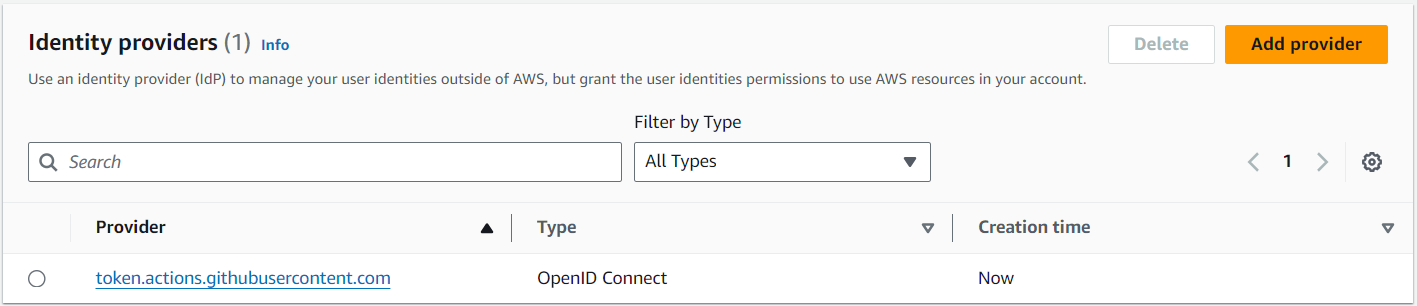
\includegraphics[width=1\columnwidth]{validation/1_Identity_provider.png}
    \captionof{figure}{GitHub identity provider}
    \label{fig:1_Identity_provider}
    \endgroup
\end{center}
An IAM role has been set up to authorise only the project's GitHub repository to access resources. A policy is linked to limit the actions allowed on the resources (figure \ref{fig:2_OIDCRole}).
\begin{center}
    \begingroup
    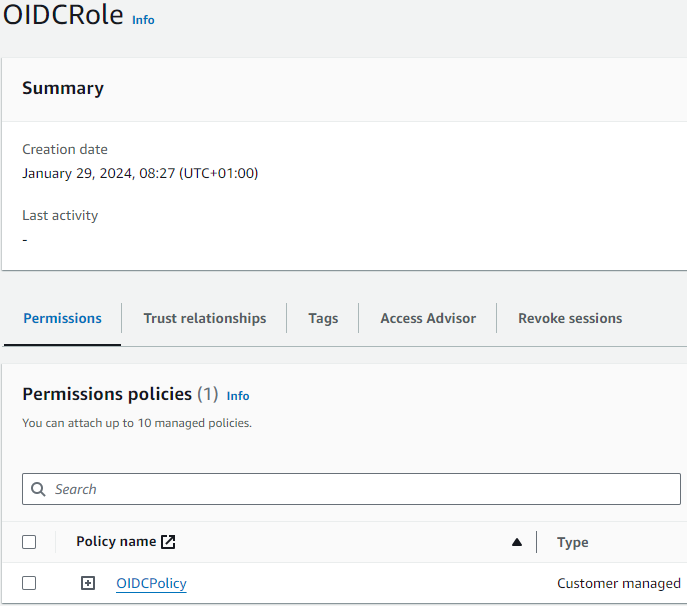
\includegraphics[width=.8\columnwidth]{validation/2_OIDCRole.png}
    \captionof{figure}{IAM OIDC role}
    \label{fig:2_OIDCRole}
    \endgroup
\end{center}
The secret and visible variables that need to be configured have been added to the GitHub repository (figures \ref{fig:3_SecretVar_GitHub} and \ref{fig:3_Var_GitHub}).
\begin{center}
    \begingroup
    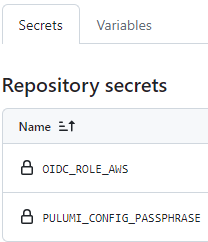
\includegraphics[width=.25\columnwidth]{validation/3_SecretVar_GitHub.png}
    \captionof{figure}{GitHub secret variables}
    \label{fig:3_SecretVar_GitHub}
    \endgroup
\end{center}
\begin{center}
    \begingroup
    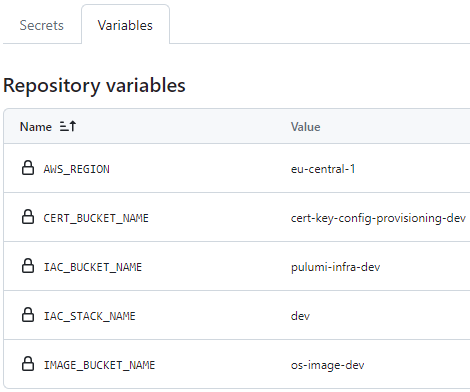
\includegraphics[width=.5\columnwidth]{validation/3_Var_GitHub.png}
    \captionof{figure}{GitHub visible variables}
    \label{fig:3_Var_GitHub}
    \endgroup
\end{center}
The configuration file for the Pulumi tool was configured by specifying the \gls{aws} account ID and the region (figure \ref{fig:4_Set_Pulumi_Stack}).
\begin{center}
    \begingroup
    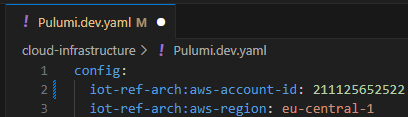
\includegraphics[width=.55\columnwidth]{validation/4_Set_Pulumi_Stack.png}
    \captionof{figure}{Pulumi configuration file (development environment)}
    \label{fig:4_Set_Pulumi_Stack}
    \endgroup
\end{center}
Finally, the serial numbers of the devices authorised to be provisioned have been listed. In this case, only a Raspberry Pi 4 is authorised (figure \ref{fig:5_Set_Allowlist}).
\begin{center}
    \begingroup
    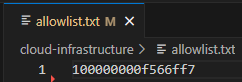
\includegraphics[width=.3\columnwidth]{validation/5_Set_Allowlist.png}
    \captionof{figure}{Embedded systems allowlist}
    \label{fig:5_Set_Allowlist}
    \endgroup
\end{center}

\section{\texorpdfstring{\acrshort{ci}/\acrshort{cd}}{} pipeline}

% -- Your text goes here --
After the previous configuration, the project was pushed into the GitHub repository. The \acrshort{ci}/\acrshort{cd} pipeline started automatically, beginning with the deployment of the \gls{cloud_infrastructure}. All tasks were completed successfully. The different times for each workflow can be seen on the right-hand side of figure \ref{fig:6_Workflows}. Total process time is just over 10 minutes.
\begin{center}
    \begingroup
    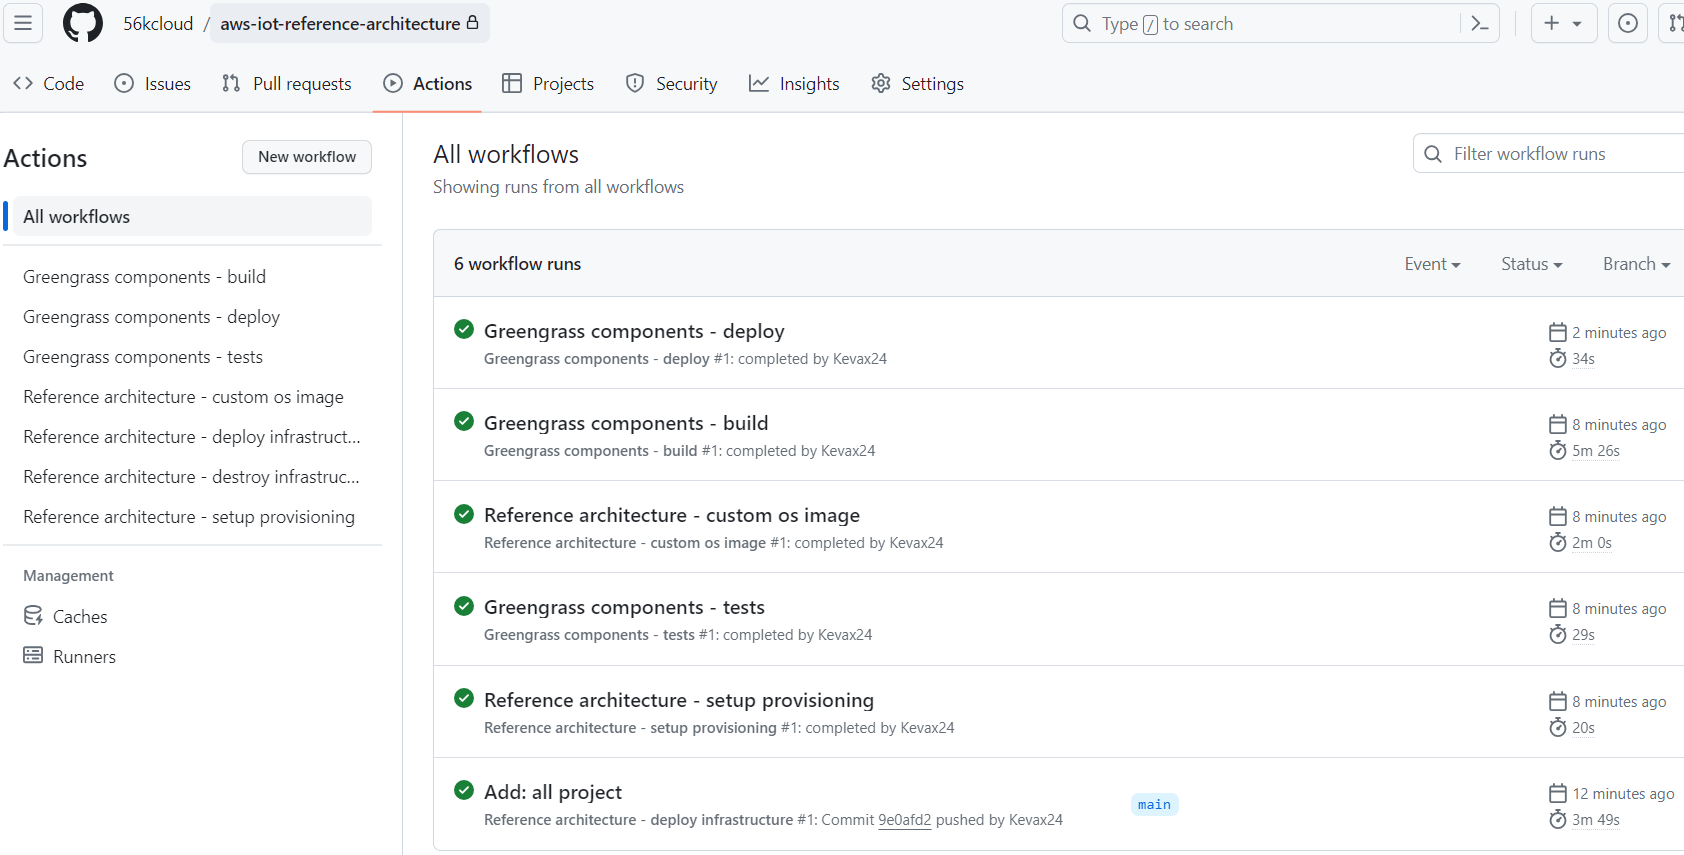
\includegraphics[width=1\columnwidth]{validation/6_Workflows.png}
    \captionof{figure}{Successful workflows}
    \label{fig:6_Workflows}
    \endgroup
\end{center}
The \gls{cloud_infrastructure} has been deployed on the development account specified and in the \textit{eu-central-1} region. The configuration for the provisioning of the embedded systems was carried out correctly with the creation of the \acrshort{os} image. The base image used is \textit{Raspberry Pi \acrshort{os} Lite} based on the Debian distribution.

At the same time, the applications were tested, including the led application, the button application and the certificate rotation application. Five Greengrass components were created and published in \gls{aws}. These components were also deployed.

\section{\texorpdfstring{\Gls{cloud_infrastructure}}{} deployment}

% -- Your text goes here --
All the resources described in Pulumi have been created correctly. In this sequel, they are not all mentioned and presented in images due to the sheer number of resources. An example is shown in figure \ref{fig:10_Infra_S3} where the S3 buckets have been created. There is the storage space for the state of the infrastructure, another for the provisioning configuration and finally one where the \acrshort{os} image is stored.
\begin{center}
    \begingroup
    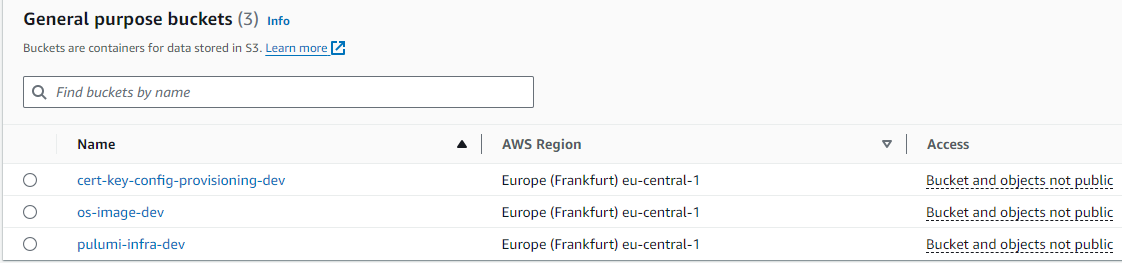
\includegraphics[width=1\columnwidth]{validation/10_Infra_S3.png}
    \captionof{figure}{S3 buckets}
    \label{fig:10_Infra_S3}
    \endgroup
\end{center}
The \acrshort{iot} device group has been created under the \textit{GreengrassGroup} name. Two policies were created for \gls{provisioning} and for interactions once provisioned (figure \ref{fig:10_Infra_IoT_Policies}). The claim certificate has also been prepared and linked to the \gls{provisioning} policy.
\begin{center}
    \begingroup
    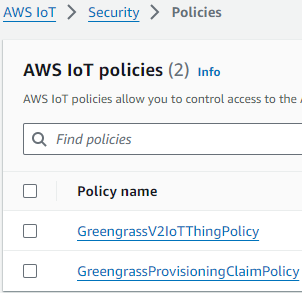
\includegraphics[width=.3\columnwidth]{validation/10_Infra_IoT_Policies.png}
    \captionof{figure}{\acrshort{iot} policies}
    \label{fig:10_Infra_IoT_Policies}
    \endgroup
\end{center}
The Greengrass components have been successfully published (figure \ref{fig:10_Infra_IoT_Components}). Docker images of the applications are also available in the Amazon \acrshort{ecr} service.
\begin{center}
    \begingroup
    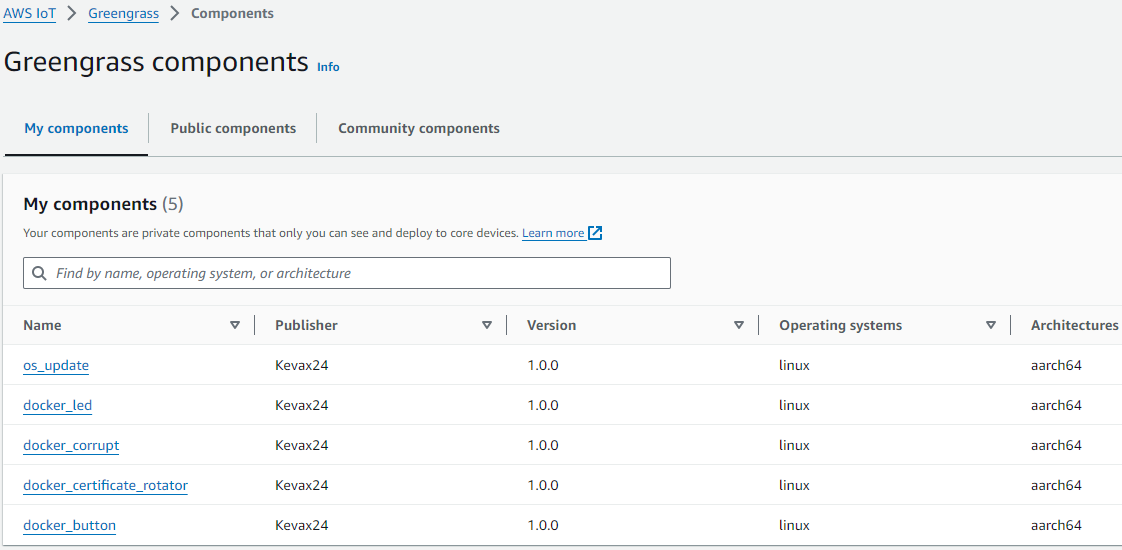
\includegraphics[width=1\columnwidth]{validation/10_Infra_IoT_Components.png}
    \captionof{figure}{Greengrass components}
    \label{fig:10_Infra_IoT_Components}
    \endgroup
\end{center}
A deployment service is ready to deploy applications as soon as devices are provisioned. It targets the group created (figure \ref{fig:10_Infra_IoT_Deployment}).
\begin{center}
    \begingroup
    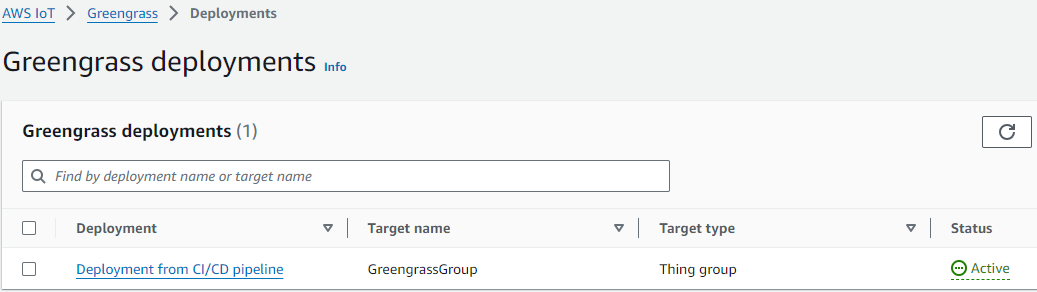
\includegraphics[width=1\columnwidth]{validation/10_Infra_IoT_Deployment.png}
    \captionof{figure}{\gls{aws} \acrshort{iot} Greengrass Deployment}
    \label{fig:10_Infra_IoT_Deployment}
    \endgroup
\end{center}

\section{\texorpdfstring{\Gls{provisioning}}{} a Raspberry Pi 4}

% -- Your text goes here --
The integration of an \acrshort{iot} device was a success. A Raspberry Pi 4 was provisioned. The \acrshort{os} image was first downloaded from the S3 bucket. It was then flashed into an SD card (figure \ref{fig:7_Flashing_SDCard}).
\begin{center}
    \begingroup
    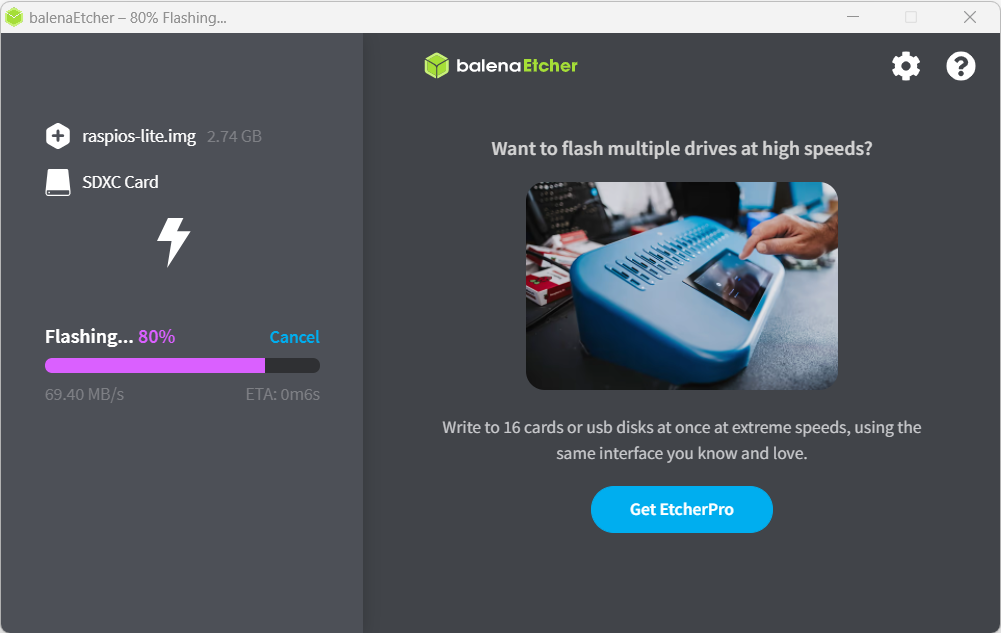
\includegraphics[width=.9\columnwidth]{validation/7_Flashing_SDCard.png}
    \captionof{figure}{\acrshort{os} image flashing}
    \label{fig:7_Flashing_SDCard}
    \endgroup
\end{center}
The Raspberry Pi 4 was then powered up and booted for the first time. All the software was installed and \gls{provisioning} was successfully completed (figure \ref{fig:8_Provisioning_Done}).
\begin{center}
    \begingroup
    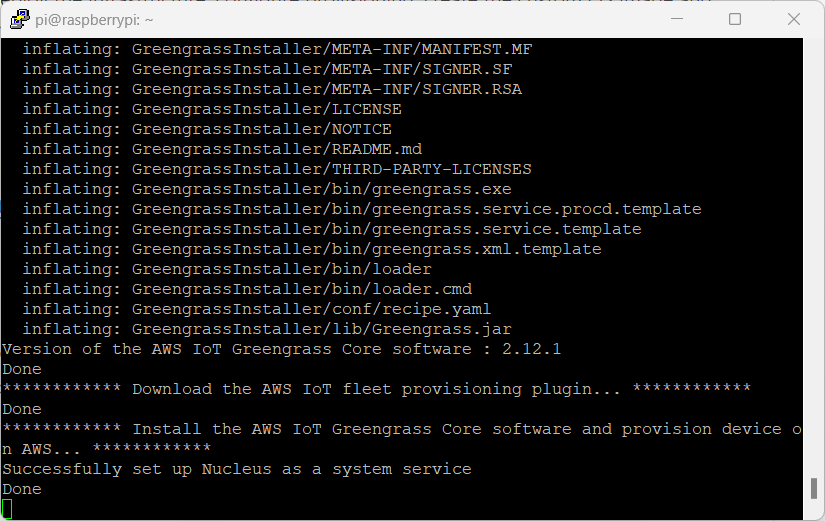
\includegraphics[width=.9\columnwidth]{validation/8_Provisioning_Done.png}
    \captionof{figure}{End of \gls{provisioning} on the device}
    \label{fig:8_Provisioning_Done}
    \endgroup
\end{center}
\Gls{provisioning} is confirmed in figure \ref{fig:8_Provisioned_AWS}. \gls{aws} has created a digital twin of this device on the \gls{aws} \acrshort{iot} service. The name corresponds to its serial number. It is linked to the group created earlier. A unique X.509 certificate has been provided.
\begin{center}
    \begingroup
    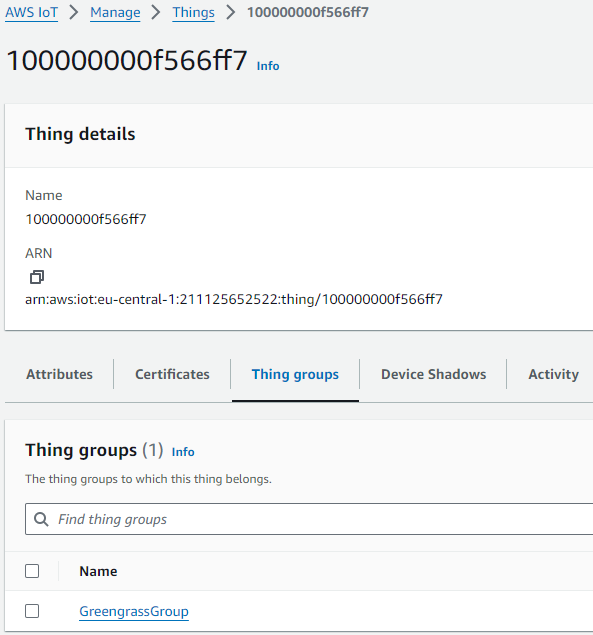
\includegraphics[width=.6\columnwidth]{validation/8_Provisioned_AWS.png}
    \captionof{figure}{Confirmed \gls{provisioning} on \gls{aws}}
    \label{fig:8_Provisioned_AWS}
    \endgroup
\end{center}

\subsection{Adding a second Raspberry Pi 4}
A second Raspberry Pi 4 has been successfully provisioned. Its serial number has been added to the list of authorised devices. A proof of its digital twin can be seen in figure \ref{fig:21_SecondProvisionRPi}.
\begin{center}
    \begingroup
    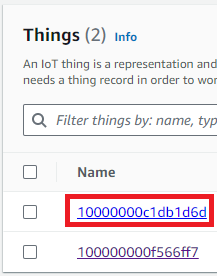
\includegraphics[width=.25\columnwidth]{validation/21_SecondProvisionRPi.png}
    \captionof{figure}{Second provisioning confirmed on \gls{aws}}
    \label{fig:21_SecondProvisionRPi}
    \endgroup
\end{center}
The components have been deployed correctly. A message exchange can be seen on the \gls{aws} \acrshort{mqtt} client interface (figure \ref{fig:21_SecondRPiMQTT}). A new blinking frequency was sent to the second Raspberry Pi 4 and a message from it was returned to \gls{aws} \acrshort{iot}.
\begin{center}
    \begingroup
    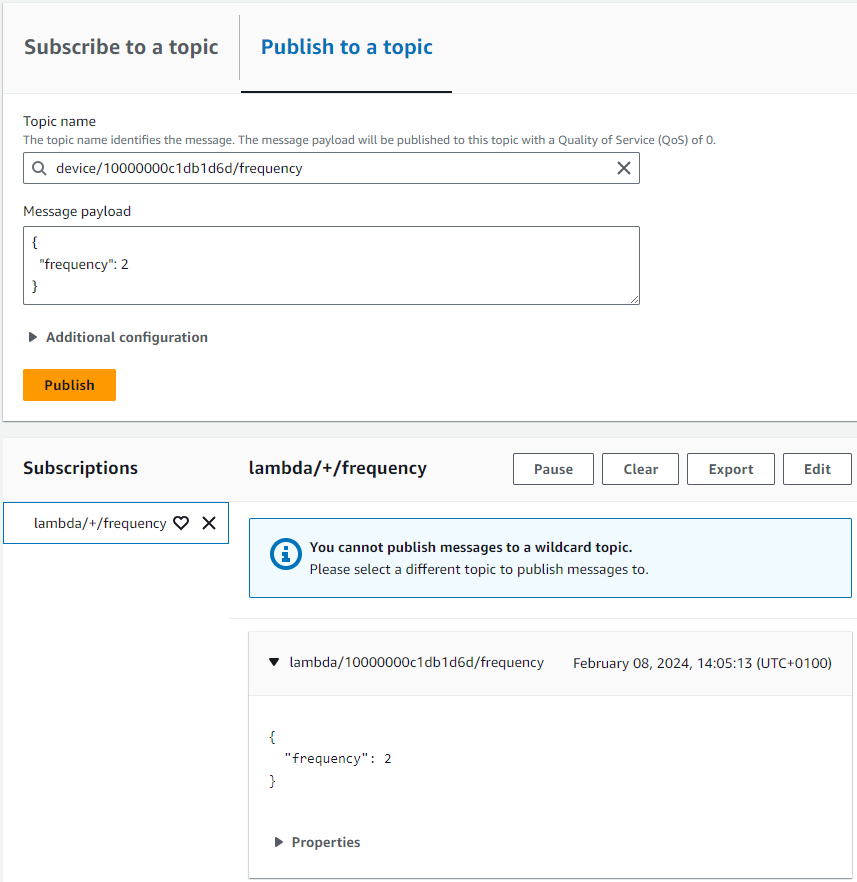
\includegraphics[width=.8\columnwidth]{validation/21_SecondRPiMQTT.png}
    \captionof{figure}{Exchanging \acrshort{mqtt} messages with the second Raspberry Pi 4}
    \label{fig:21_SecondRPiMQTT}
    \endgroup
\end{center}

\section{Applications}

% -- Your text goes here --
All the applications were deployed on the Raspberry Pi 4. As soon as it was provisioned, the deployment started. This can be seen in figure \ref{fig:9_Deployment_InProgress}.
\begin{center}
    \begingroup
    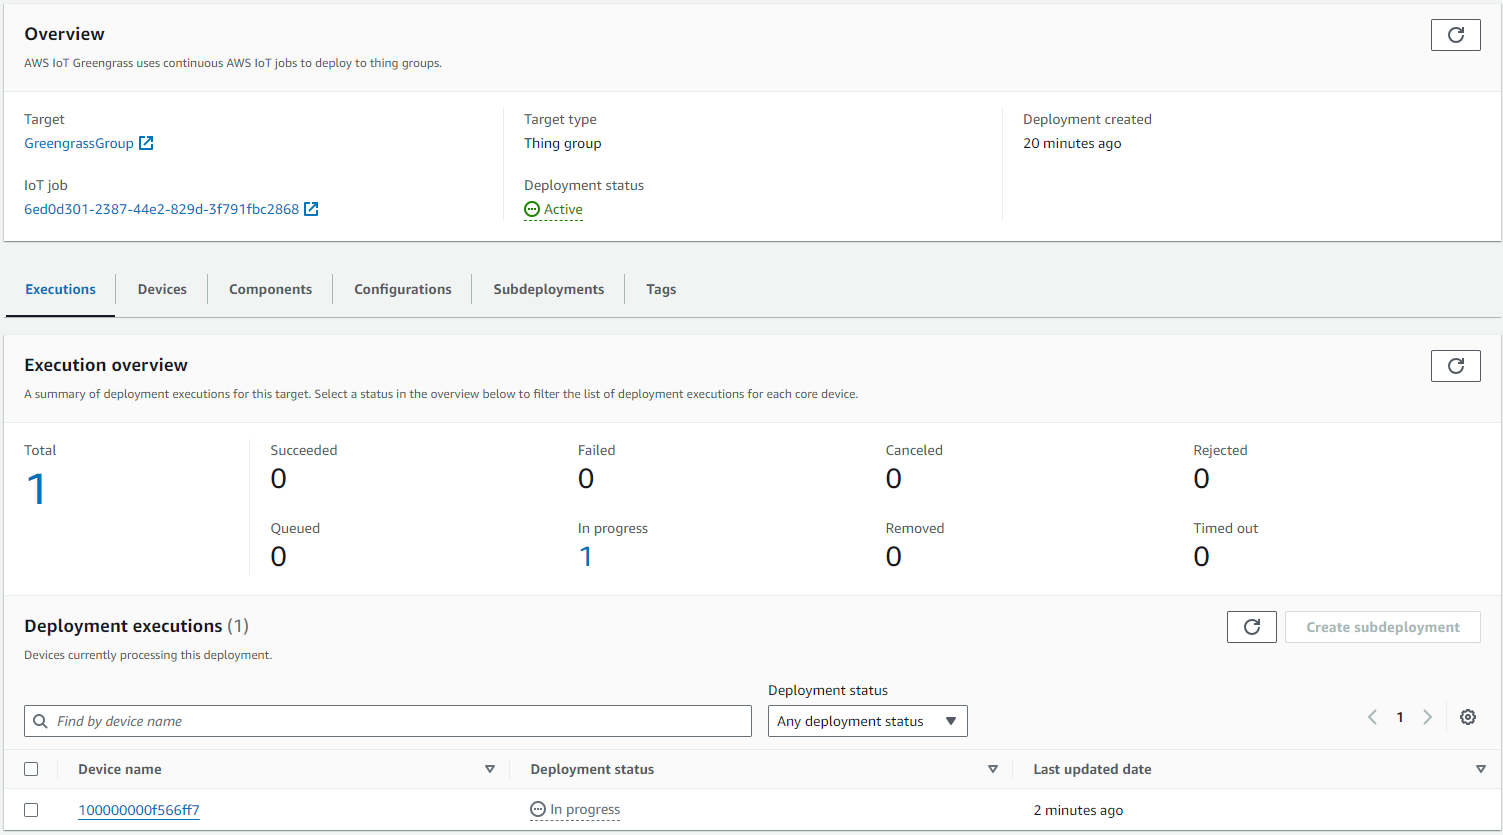
\includegraphics[width=1\columnwidth]{validation/9_Deployment_InProgress.png}
    \captionof{figure}{Deployment of Greengrass components in progress}
    \label{fig:9_Deployment_InProgress}
    \endgroup
\end{center}
Deployment took just a few minutes. The Greengrass components acting as intermediaries for the applications can be seen in figure \ref{fig:11_Components_Running}. The dependencies are also installed in addition to the Greengrass nucleus \textit{aws.greengrass.Nucleus}.
\begin{center}
    \begingroup
    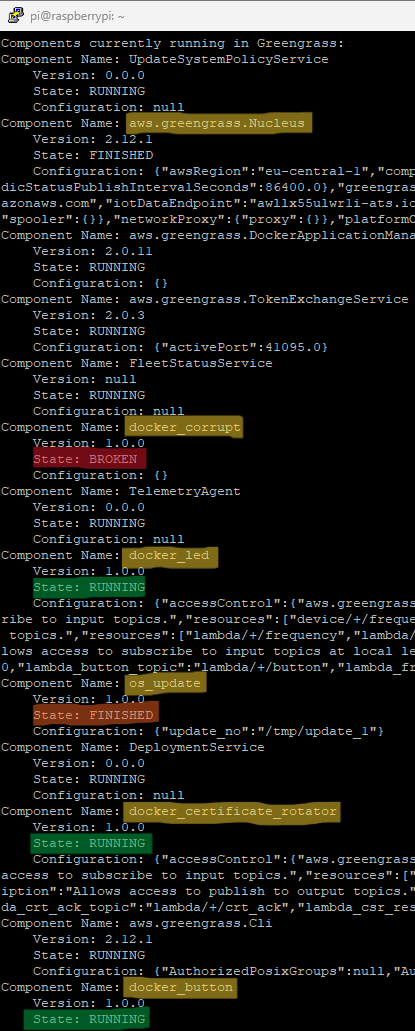
\includegraphics[width=.5\columnwidth]{validation/11_Components_Running.png}
    \captionof{figure}{Greengrass components deployed}
    \label{fig:11_Components_Running}
    \endgroup
\end{center}
It is possible to see an overview of the Raspberry Pi 4 on \gls{aws} as shown in figure \ref{fig:13_DeviceHealth}. Its state of health is poor because a component failed when it was launched. In fact, the corrupted component was unable to start up correctly and was interrupted. The other components are in a state of execution or completion.
\begin{center}
    \begingroup
    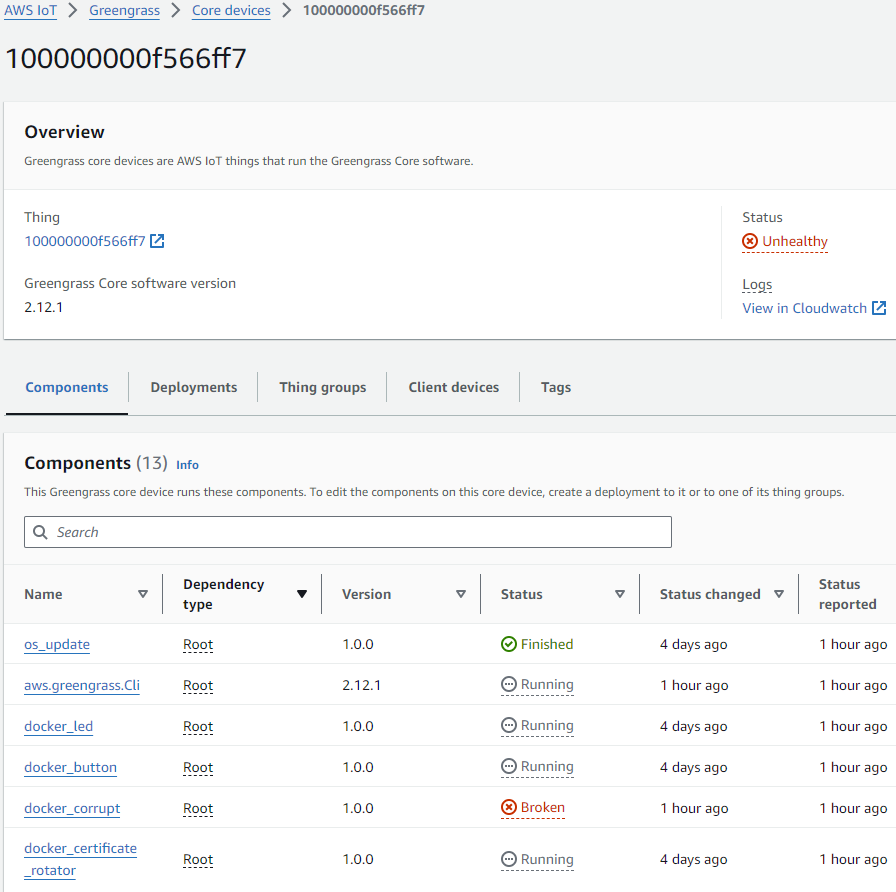
\includegraphics[width=1\columnwidth]{validation/13_DeviceHealth.png}
    \captionof{figure}{Overview of the Raspberry Pi 4 from \gls{aws}}
    \label{fig:13_DeviceHealth}
    \endgroup
\end{center}

\subsection{Applications interaction}
The applications were then tested. The first was the led application. The \gls{aws} web interface was used to send \acrshort{mqtt} messages and view the data received. A message is sent to the Raspberry Pi 4 to change its led blinking frequency. A response was sent back to \gls{aws} \acrshort{iot} in another field including the new frequency. A proof can be found in figure \ref{fig:12_FrequencyChange}.
\begin{center}
    \begingroup
    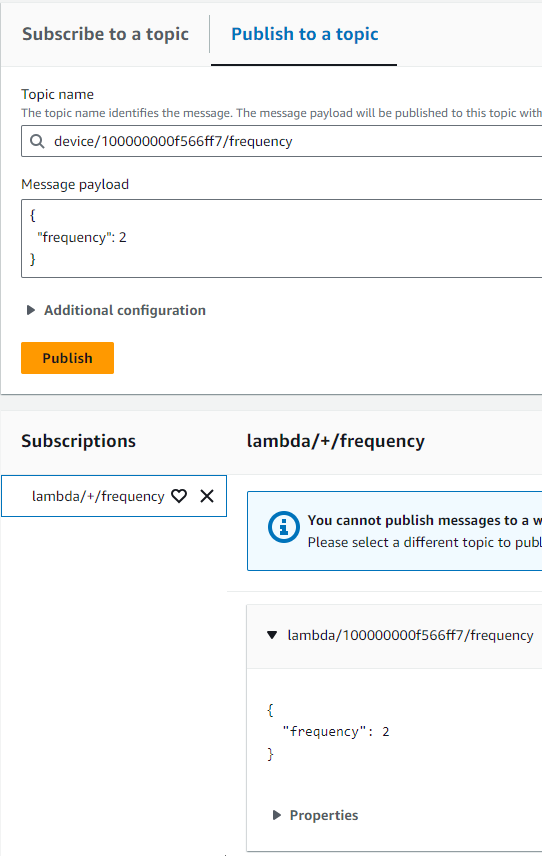
\includegraphics[width=.5\columnwidth]{validation/12_FrequencyChange.png}
    \captionof{figure}{Frequency change on \gls{aws}}
    \label{fig:12_FrequencyChange}
    \endgroup
\end{center}
Figure \ref{fig:12_LedApp_Log} shows the led application output message thread. It is possible to view different frequencies received on the Raspberry Pi 4.
\begin{center}
    \begingroup
    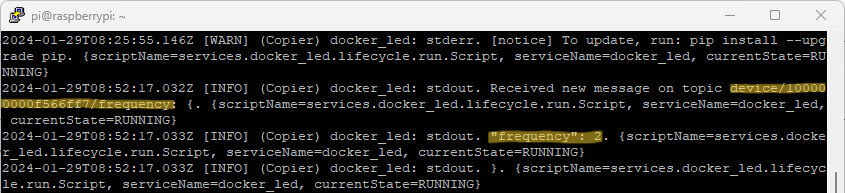
\includegraphics[width=1\columnwidth]{validation/12_LedApp_Log.png}
    \captionof{figure}{Frequency change on the Raspberry Pi 4}
    \label{fig:12_LedApp_Log}
    \endgroup
\end{center}
The button application was also tested. The external button on the Raspberry Pi 4 was pressed twice. \acrshort{mqtt} messages were transmitted to the led application locally and then published to \gls{aws} \acrshort{iot}. The messages can be seen in figure \ref{fig:12_ButtonChange}. The first press deactivates the blinking of the led and the second reactivates it.
\begin{center}
    \begingroup
    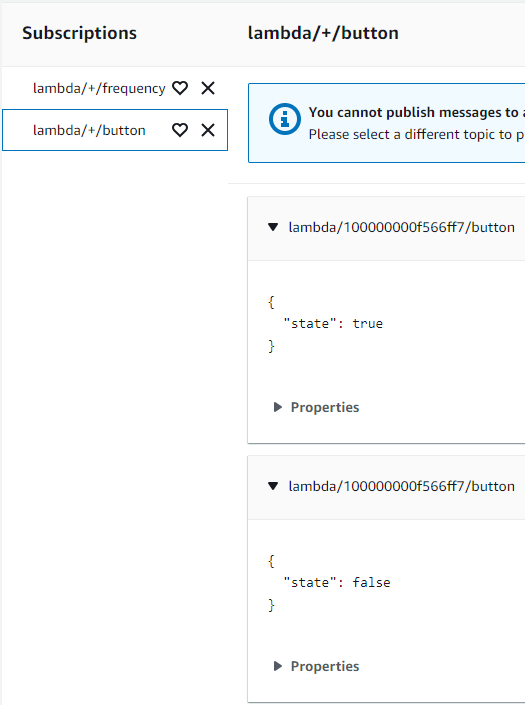
\includegraphics[width=.5\columnwidth]{validation/12_ButtonChange.png}
    \captionof{figure}{Blink status changes on \gls{aws}}
    \label{fig:12_ButtonChange}
    \endgroup
\end{center}
Figure \ref{fig:12_LedApp_Log_button} shows the output message thread of the led application. It is possible to view the \acrshort{mqtt} messages received from the button application on the Raspberry Pi 4.
\begin{center}
    \begingroup
    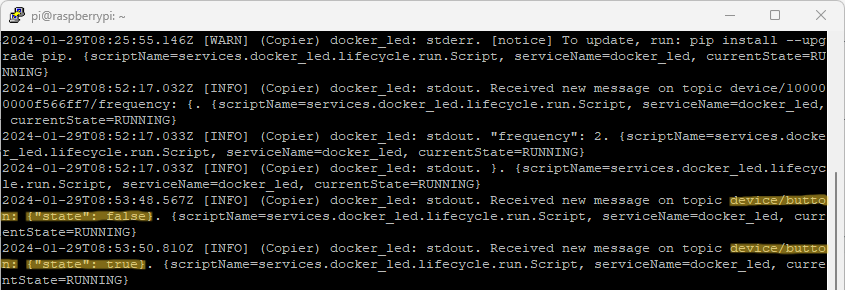
\includegraphics[width=1\columnwidth]{validation/12_LedApp_Log_button.png}
    \captionof{figure}{Blink status changes on the Raspberry Pi 4}
    \label{fig:12_LedApp_Log_button}
    \endgroup
\end{center}
Finally, the certificate was rotated. The triggering of a change alert was simulated from the \gls{aws} \acrshort{mqtt} interface by requesting the creation of \acrshort{csr} on the Raspberry Pi 4. Several \acrshort{mqtt} messages were exchanged. These are partly visible from the \gls{aws} interface in figure \ref{fig:12_CertRotate}. When analysing the digital twin, the certificate identifier was changed, proving that the rotation had indeed taken place. The Greengrass service was also restarted to take the new certificate into account.
\begin{center}
    \begingroup
    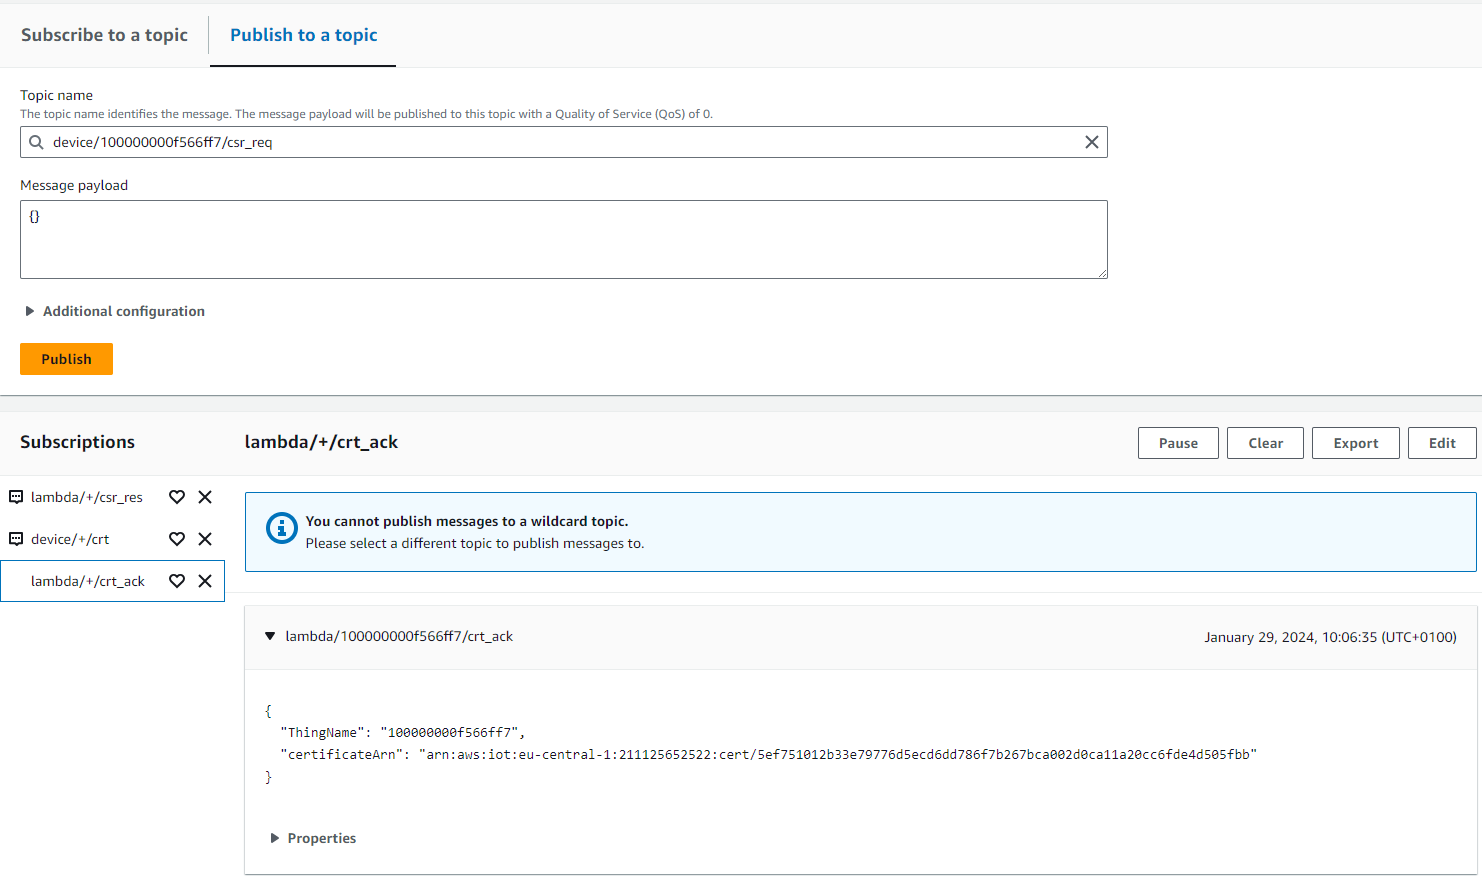
\includegraphics[width=1\columnwidth]{validation/12_CertRotate.png}
    \captionof{figure}{Certificate rotation on \gls{aws}}
    \label{fig:12_CertRotate}
    \endgroup
\end{center}
Figure \ref{fig:12_CertRotate_Log} shows the output message thread of the certificate rotation application. It is possible to view the \acrshort{mqtt} messages received from \gls{aws}. A request for \acrshort{csr} has been received as well as the new certificate.
\begin{center}
    \begingroup
    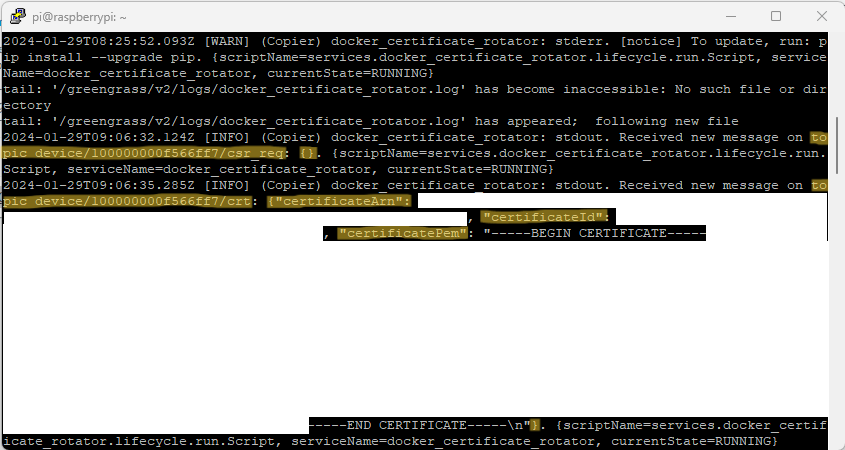
\includegraphics[width=1\columnwidth]{validation/12_CertRotate_Log.png}
    \captionof{figure}{Certificate rotation on the Raspberry Pi 4}
    \label{fig:12_CertRotate_Log}
    \endgroup
\end{center}
Due to the incorrect platform specified for the corrupted application, it was unable to start up correctly. This is clearly shown in figure \ref{fig:12_CorruptApp_Log}. Greengrass tries to start the application three times before stopping.
\begin{center}
    \begingroup
    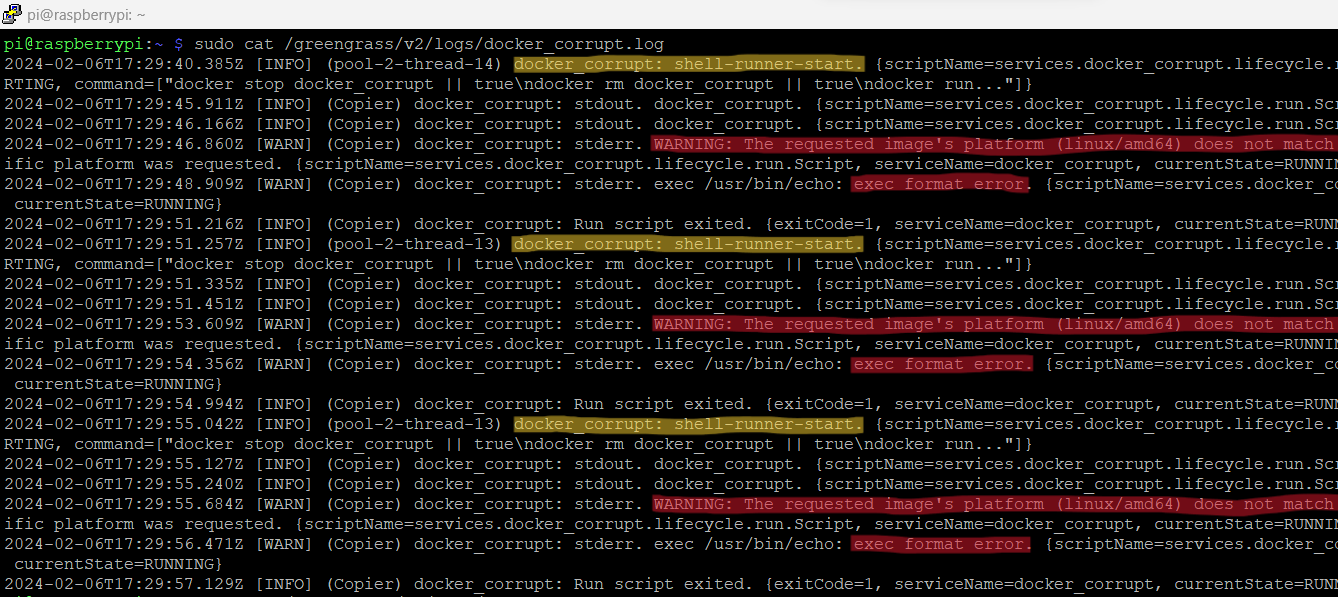
\includegraphics[width=1\columnwidth]{validation/12_CorruptApp_Log.png}
    \captionof{figure}{Launching the corrupt application on the Raspberry Pi 4}
    \label{fig:12_CorruptApp_Log}
    \endgroup
\end{center}
During testing of the components, an additional observation was made. If a component is corrupted and subsequently deployed with updates to other components, these components will retain the old version. As long as the corrupted application is not corrected, all the components remain frozen on the last version deployed, and not on the last version of the component.

\subsection{Updating an application}
In order to test the deployment of an update, the corrupted application was corrected by specifying the correct architecture. The Greengrass component has been updated since it has changed version (figure \ref{fig:14_NewComponentVersion}).
\begin{center}
    \begingroup
    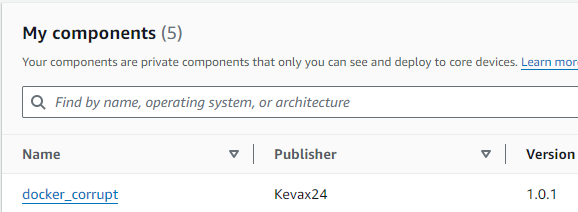
\includegraphics[width=.8\columnwidth]{validation/14_NewComponentVersion.png}
    \captionof{figure}{New version of the corrupted application on \gls{aws}}
    \label{fig:14_NewComponentVersion}
    \endgroup
\end{center}
Looking at the Raspberry Pi 4 console in figure \ref{fig:14_CorruptApp_updated}, the application ran correctly. A text was printed as agreed.
\begin{center}
    \begingroup
    \includegraphics[width=1\columnwidth]{validation/14_CorruptApp_updated.png}
    \captionof{figure}{Preview of the corrupted application on the Raspberry Pi 4}
    \label{fig:14_CorruptApp_updated}
    \endgroup
\end{center}
Now that no components have been corrupted, the health of the \acrshort{iot} device is good. This was noted on the \gls{aws} console.

\subsection{\texorpdfstring{\acrshort{os}}{} update}
An update simulation was tested. The commands written were executed correctly and the Raspberry Pi 4 rebooted automatically without restarting the command lines. Evidence of this can be seen in figure \ref{fig:20_os_update}. The first time it was run, the \textit{apt-get update} command was issued, followed by the restart command. When the Greengrass component is launched a second time, it is noted that the update has already taken place.
\begin{center}
    \begingroup
    \includegraphics[width=1\columnwidth]{validation/20_os_update.png}
    \captionof{figure}{Behaviour of the \acrshort{os} update application}
    \label{fig:20_os_update}
    \endgroup
\end{center}

\section{\texorpdfstring{\Gls{cloud_infrastructure}}{} destruction}

% -- Your text goes here --
The \gls{cloud_infrastructure} destruction was tested. To do this, the corresponding workflow was launched manually from the GitHub Actions console and passed successfully (figure \ref{fig:15_DestroyInfra}). It takes about 4 minutes. All the resources created by the Pulumi tool have been deleted. The Raspberry Pi 4 remains provisioned with its unique certificate. The claim certificate remains available in the S3 bucket with its private key. The Greengrass components have not been removed either.
\begin{center}
    \begingroup
    \includegraphics[width=.6\columnwidth]{validation/15_DestroyInfra.png}
    \captionof{figure}{\Gls{cloud_infrastructure} destruction successfully completed}
    \label{fig:15_DestroyInfra}
    \endgroup
\end{center}
The Raspberry Pi 4's digital twin is still contained within \gls{aws} \acrshort{iot}. However, it has lost any policy for interacting with the \gls{cloud}. The \acrshort{mqtt} connection is therefore interrupted except locally on the device between the components. This was proven by pressing the external button on the Raspberry Pi 4 just once. The led stopped blinking and no status message was received on \gls{aws} \acrshort{iot}.

\section{Management of authorised embedded systems}

% -- Your text goes here --
\subsection{Infrastructure deployment with a provisioned embedded system}
Following the logic of the tests, the infrastructure was redeployed with the Raspberry Pi 4 already provisioned. Its digital twin was attached to the group of devices and to an \acrshort{iot} policy. \acrshort{mqtt} communication with the \gls{cloud} is now back up and running. Figure \ref{fig:16_AttachExistingThing} shows the attachment of the device to the new \gls{cloud_infrastructure} in the GitHub Actions console.
\begin{center}
    \begingroup
    \includegraphics[width=1\columnwidth]{validation/16_AttachExistingThing.png}
    \captionof{figure}{Integration of Raspberry Pi 4 already provisioned}
    \label{fig:16_AttachExistingThing}
    \endgroup
\end{center}

\subsection{Deleting a provisioned embedded system}
It is possible to remove a device from the \gls{aws} \gls{cloud} by deleting its serial number from the list of authorised devices. The serial number of the provisioned Raspberry Pi 4 has therefore been removed and this change has been pushed into Git. By following the GitHub Actions console in figure \ref{fig:17_RemoveThing}, it is possible to confirm that the device has been deleted. By browsing the \gls{aws} console, its digital twin no longer exists and no \acrshort{mqtt} message reaches \gls{aws} \acrshort{iot}.
\begin{center}
    \begingroup
    \includegraphics[width=1\columnwidth]{validation/17_RemoveThing.png}
    \captionof{figure}{Removal of the provisioned Raspberry Pi 4}
    \label{fig:17_RemoveThing}
    \endgroup
\end{center}
For this Raspberry Pi 4 to be provisioned again, it must be authorised again and its SD card must be flashed again with the \acrshort{os} image.

\subsection{Unauthorised provisioning of an embedded system}
This same Raspberry Pi 4 was tested for reintegration into the \gls{cloud_infrastructure} without being authorised. Its serial number was therefore not included in the list of authorised devices. Its SD card was flashed with the same \acrshort{os} image as for all the other tests carried out. Both software, Docker Engine and \gls{aws} \acrshort{iot} Greengrass, were successfully installed. During the provisioning attempt, the Lambda function, triggered at each attempt, detected that this Raspberry Pi 4 was not authorised to be provisioned. Its certificate, which had been prepared and was supposed to be delivered to it, was therefore left waiting to be activated. After a while, the certificate disappears. This can be seen in figure \ref{fig:18_CertificatPending}.
\begin{center}
    \begingroup
    \includegraphics[width=1\columnwidth]{validation/18_CertificatPending.png}
    \captionof{figure}{Certificat en attente d'activation}
    \label{fig:18_CertificatPending}
    \endgroup
\end{center}

\section{Provisioning of other Arm SystemReady certified embedded systems}

% -- Your text goes here --

\section{\texorpdfstring{\Gls{cloud_infrastructure}}{} cost}

% -- Your text goes here --
An assessment of the costs of the \gls{aws} \gls{cloud_infrastructure} was carried out in order to understand the monthly and annual expenses to be expected. This estimate was carried out using the \gls{aws} Pricing Calculator. The estimate is shown in figure \ref{fig:19_CostEstimate}.
\begin{center}
    \begingroup
    \includegraphics[width=1\columnwidth]{validation/19_CostEstimate.png}
    \captionof{figure}{\Gls{cloud_infrastructure} cost estimate}
    \label{fig:19_CostEstimate}
    \endgroup
\end{center}
The evaluation is based on a number of factors, assuming that it is the cost of the infrastructure in the production environment. The region chosen is Frankfurt (\textit{eu-central-1}). A fleet of 100 embedded systems is considered.

\gls{aws} \acrshort{iot} Core is a high-cost service. Here is a list of factors taken into account :
\begin{itemize}
    \item Number of devices : 100
    \item Protocol : \acrshort{mqtt}
    \item Average size per message : 10 kB
    \item Number of messages per month per device : 43'800 (1 par minute)
    \item Number of rules triggered per month per device : 43'800
\end{itemize}
Each device sends one 10 kB \acrshort{mqtt} message per minute. Each message received in \gls{aws} \acrshort{iot} Core triggers a rule that diverts the message to another service. For example, Lambda functions can be called by these rules depending on the message heading.

\gls{aws} \acrshort{iot} Greengrass is the most expensive service. Here are the factors taken into consideration:
\begin{itemize}
    \item Number of devices : 100
    \item Activity period per month : 43'800 minutes (100\% activity)
    \item Number of \acrshort{mqtt} topics : 1000
\end{itemize}
With 1000 \acrshort{mqtt} topics, each device can have 10 unique topics each.

The \gls{aws} \acrshort{iot} Device Defender service is used to perform a daily audit by monitoring a single aspect, namely the expiry of certificates. The cost is virtually insignificant.

The \gls{aws} Lambda service is used to execute operations when a function is triggered by a received message. It is estimated that each message received triggers a function, with a total of 4''380'000 messages sent per month for the fleet of 100 embedded systems. The average execution time for a Lambda function is one second.

Amazon \acrfull{ecr} is used to store the Docker images generated for the applications developed. A monthly storage limit of 50 GB has been defined. None of the application images in this project exceeds 400 MB. Therefore, there can be up to 125 images of this size to reach the 50 GB limit.

Amazon S3 is also used for storage, with three S3 buckets in use. The bucket containing the OS image for this reference architecture weighs 2.6 GB. The total of the three buckets remains at 2.6 GB, indicating that the Pulumi files on the state of the infrastructure, in addition to the provisioning files, do not exceed 100 MB.

The Amazon SNS service used in the reference architecture is not taken into account, as it is triggered every so many years (a certificate has a lifetime of several years by default). Consequently, its cost is negligible.
% ------------------------------------------------------------------------------
% It describes the means used to manage a project.
% ------------------------------------------------------------------------------

\opt{never}{\addbibresource{03-tail/bibliography.bib}} % to make citation found in most IDE

\chapter{Project methodology}
\label{chap:methodology}

% -- Your text goes here --
Project methodology consists of describing the means used to manage a project. In this chapter, the concept of agility is described in order to explain how the iterative process works. In addition, the \gls{kanban} methodology is described in detail to explain the time aspect of the tasks to be carried out. Finally, the various tools used are discussed.

\minitoc
\newpage

% ------------------------------------------------------------------------------
\section{Agile methodology}

% -- Your text goes here --
Agile methodology is the main project management method used in this work. It enables the project to be managed from the specifications to the final product. The idea for this method was conceived in the 70s or even before \cite{abbas_historical_2008}.  The idea was to change the development process in software engineering by using iterative techniques. Traditional methods worked with sequential techniques, often called Waterfall. Figure \ref{fig:waterfall_vs_scrum} shows the difference between these two approaches.
\begin{center}
    \begingroup
    \includegraphics[width=1\columnwidth]{methodology/waterfall_vs_scrum.pdf}
    \captionof{figure}{Sequential and iterative process \cite{course_MA_ITProMan}}
    \label{fig:waterfall_vs_scrum}
    \endgroup
\end{center}
The Waterfall methodology is considered cumbersome. There are deliverables after each phase. Approval is required before moving on to the next phase. It is difficult to go backwards (by moving up the phases). Professors explained this very well during a Masters course given at the \gls{hes} \cite{course_MA_ITProMan}. They added that this method is best used in very large projects where it is difficult to split teams into small groups to work iteratively.

These same teachers \cite{course_MA_ITProMan} described the agile methodology as follows:
\begin{quote}
    \textit{"AGILE" is about values and principles, not practices, but many practices support them. It's not about doing agile, it's about being agile}.
\end{quote}
Several agile process frameworks were created before the 2000s. Examples include \gls{scrum}, XP, RUP, etc. Between the 11th and the 13th of February 2001, 17 people from these different frameworks met to find an alternative to cumbersome, documentation-driven software development processes. They created the agile software development manifesto \cite{manifesto_agile} :
\begin{itemize}
    \item[] \textit{Individuals and interactions over processes and tools}
    \item[] \textit{Working software over comprehensive documentation}
    \item[] \textit{Customer collaboration over contract negotiation}
    \item[] \textit{Responding to change over following a plan}
\end{itemize}
The central principle of agile is to have very rapid iterations to build the first business values. The customer is at the centre of the process thanks to frequent communication with the development team \cite{course_MA_ITProMan}. The process framework chosen for this project is \gls{scrum}. It is very well suited to small projects with small teams. It enables the first software prototypes to be delivered quickly. It adapts easily to changes, unlike a sequential method. It is also based on experience. The idea is to learn continuously through iterations. This is an important point in terms of learning from new developments in the project. This is one of the most popular agile methods. This approach was launched in 1995 by Ken Schwaber and Jeff Sutherland \cite{scrum_guide_site}.

\subsection{\Gls{scrum} roles}
Figure \ref{fig:scrum_roles} shows the different roles in a \gls{scrum} team.
\begin{center}
    \begingroup
    \includegraphics[width=.8\columnwidth]{methodology/scrum_roles.pdf}
    \captionof{figure}{\Gls{scrum} roles}
    \label{fig:scrum_roles}
    \endgroup
\end{center}
A \gls{scrum} guide has been written by Jeff Sutherland and Ken Schwaber to explain the rules \cite{scrum_guide}. First of all, there is the \acrfull{po}. This is the customer's spokesperson. It is he who defines the product's functionalities. They are recorded in a Product Backlog in the form of tasks. He must manage these tasks by prioritising some of them. He is also responsible for the value and return on investment (\acrshort{roi}) of the product. The development team is generally a small one (around seven people \cite{course_MA_ITProMan}). It is capable of self-management. There are no specific roles or positions. Developers have to deal with tasks that are chosen from the Sprint Backlog. Finally, the \gls{scrum} Master is required to be of service to the team. He accompanies the team of developers and prevents obstacles from getting in the way of progress. It is the \gls{scrum} Master who establishes the practices and rules of \gls{scrum}.

\subsection{\texorpdfstring{\gls{scrum}}{} process}
The \gls{scrum} process is relatively simple. It follows the theory described in the official \gls{scrum} guide \cite{scrum_guide}. The life cycle is shown in figure \ref{fig:scrum_process}.
\begin{center}
    \begingroup
    \includegraphics[width=.9\columnwidth]{methodology/scrum_process.pdf}
    \captionof{figure}{\Gls{scrum} life cycle}
    \label{fig:scrum_process}
    \endgroup
\end{center}
The process is made up of multiple elements. It begins on the left of the diagram with the Product Backlog. This is a backlog that is filled by the \acrshort{po}. Since the Product Backlog is generally filled with many functionalities divided into tasks, only one part needs to be selected to be placed in the Sprint Backlog. A Sprint generally corresponds to a period of one month during which the tasks in the Sprint Backlog must be completed. During a Sprint, team meetings are organised every day. These are called Daily Meetings and usually last 15 minutes. A Daily Meeting ensures that, at least once a day, the entire team is available to get support on any problems encountered. In this project, only weekly meetings are held, depending on the distance separating the \gls{scrum} Master and the team of developers. Before each Sprint, a Sprint Planning is carried out to determine the tasks from the Product Backlog to be put into the Sprint Backlog. At the end of a Sprint, an inspection is made of how the Sprint went, with the aim of improving quality and efficiency. This is called a Sprint Retrospective. Finally, it's important to remember that at the end of each Sprint, one stage of the final product is completed. Sometimes this is called an increment.

% ------------------------------------------------------------------------------
\section{KanBan methodology}

% -- Your text goes here --
The \gls{kanban} methodology is very well integrated into \gls{scrum}. Its aim is to manage the workflow as efficiently as possible. According to the \gls{kanban} guide produced by \gls{scrum}.org \cite{kanban_guide}, several fundamental metrics should be taken into account for the flow:
\begin{itemize}
    \item[—] \textbf{\acrfull{wip}} : the number of tasks/items started and not completed.
    \item[—] \textbf{Cycle Time} : the time elapsed between the start and end of a task.
    \item[—] \textbf{Work Item Age} : the time elapsed between the start of the task and now.
    \item[—] \textbf{Throughput} : the number of tasks completed per unit of time.
\end{itemize}
The average cycle time can be predicted using Little's Law \cite{little_law}:
\begin{equation}
    average\ cycle\ time = \frac{average\ \acrshort{wip}}{average\ throughput}
\end{equation}
It explains that the more tasks there are in progress, the longer it will take to complete them. A cycle time in \gls{kanban} can be correlated to a Sprint in the \gls{scrum} methodology. Using this methodology, it is therefore possible to define the right number of tasks for each Sprint Planning. Note that the more you divide a feature into smaller tasks, the easier it will be to predict the cycle time.

\gls{kanban} does more than just limit the \acrshort{wip}. It provides a transparent display of the workflow. Tasks can be represented in a table, as shown in figure \ref{fig:kanban_example}. In this case, the table is virtual and can be viewed from anywhere by the whole \gls{scrum} team.
\begin{center}
    \begingroup
    \includegraphics[width=1\columnwidth]{methodology/kanban_example.png}
    \captionof{figure}{Example of a virtual \gls{kanban} table \cite{kanban_example}}
    \label{fig:kanban_example}
    \endgroup
\end{center}
Each label in the table corresponds to a task. A task can contain a priority level and is often assigned to a member of the \gls{scrum} team. All this is defined during Sprint Planning. The labels are categorised in columns to show their progress.


% ------------------------------------------------------------------------------
\section{Project management tools}

% -- Your text goes here --
\subsection{Version management}
Version management, embodied by tools such as Git, remains an essential part of the software development ecosystem. This practice offers a structured approach to tracking and maintaining changes to a project's code. One of the major benefits lies in its ability to keep a complete history of changes, facilitating collaboration between team members working on the same project.
\begin{center}
    \begingroup
    \includegraphics[width=0.8\columnwidth]{methodology/version_control.pdf}
    \captionof{figure}{Example of version management with two branches}
    \label{fig:version_control}
    \endgroup
\end{center}
An example of a visual representation of a project is shown in figure \ref{fig:version_control}, comprising several distinct versions and branches. Branches allow developers to work on alternative versions of the source code, facilitating parallel development, feature isolation and efficient change management without affecting the main branch.

When part of the development is considered complete, it becomes common practice to create a new version. This version freezes the current state of the project at a specific point in time, providing a clear and stable reference. This ability to create versions means that it is possible to return to previous states of the project if problems arise, whether identified by members of the development team or by external stakeholders, such as customers.

In short, version management, embodied by Git, transcends its simple function of tracking changes to become a central pillar of collaborative working, risk management and preserving the integrity of a software project. Its widespread adoption across the industry is testament to its continuing importance in delivering robust, scalable software development projects.

\subsection{\acrfull{ci} and \acrfull{cd}}

\subsection{Work packages}


% ------------------------------------------------------------------------------
\section{Formations}

% -- Your text goes here --
\begin{itemize}
    \item AWS Certified Cloud Practitioner
\end{itemize}
% ------------------------------------------------------------------------------
% A conclusion succinctly summarizes the most important results and thus represents the highlight of your Bachelor thesis.
%
% In the conclusion, you only mention information and conclusions that you have already mentioned in the course of your body text. New information is not mentioned here.
% The conclusion should have the following content:
% - Project summary
% - Comparison with the initial objectives
% - Encountered difficulties
% - Future perspectives
% ------------------------------------------------------------------------------

\opt{never}{\addbibresource{03-tail/bibliography.bib}} % to make citation found in most IDE

\chapter{Conclusions}
\label{chap:conclusions}

% -----------------------------------------------------------------------------
\section{Project summary}

% -- Your text goes here --
In summary, this project has resulted in the creation of an infrastructure that enables the fluid, automated and secure integration of \acrshort{iot} devices into an \gls{aws} \gls{cloud} environment. The reference architecture aims to simplify the integration of embedded systems within an \gls{aws} \gls{cloud_infrastructure} dedicated to the \acrshort{iot}. The devices used in this \acrshort{iot} network feature \gls{arm} architecture and are \nameref{sec:arm_systemready} certified. To improve this integration, a \acrshort{devops} approach has been put in place thanks to a continuous integration and distribution process orchestrated by GitHub Actions. The central tool for deploying the infrastructure is Pulumi, which enables \gls{aws} \gls{cloud_infrastructure} to be deployed on various environments. Python applications have been specially developed to demonstrate how integration works via \acrshort{mqtt} communication between devices and \gls{aws} \acrshort{iot}. In the \acrshort{ci}/\acrshort{cd} process, these applications are tested, published in \gls{aws} and then deployed to a fleet of devices. During these deployments, the applications run in Docker containers, ensuring greater portability. A custom \acrshort{os} image, based on Raspberry Pi \acrshort{os} Lite, has been developed, incorporating Docker for applications and \gls{aws} \acrshort{iot} Greengrass Core, which is essential for provisioning and integration.  This \acrshort{os} image is downloaded, flashed onto an SD card and inserted into an embedded system, which is automatically provisioned in a few minutes when it is first booted up. The successful integration of a first Raspberry Pi 4 has been extended to a second Raspberry Pi 4, demonstrating the scalability of the architecture. To guarantee network reliability, security mechanisms are built into the architecture, making communications within the \acrshort{iot} system even more robust and protected.

% -----------------------------------------------------------------------------
\section{Comparison with the initial objectives}

% -- Your text goes here --
The project was an overall success, achieving the main objective of designing a reference architecture to facilitate the deployment of a \gls{cloud_infrastructure} while automating the provisioning of a fleet of embedded systems. Now available as open source, this achievement provides a solid foundation for engineers looking for similar solutions. Detailed documentation accompanies the project to make it easier to understand and use.

The \nameref{subsec:cloudnative} approach and the \acrshort{devops} methodology, with continuous integration and continuous distribution, played an essential role in the development of the architecture. These choices reinforced the robustness of the architecture, simplifying its use and enabling the integration of missing elements specific to each solution.

The \gls{aws} \gls{cloud_infrastructure} is totally modular, offering the possibility of adding the additional services required for the product. The use of the Pulumi \acrshort{iac} tool, integrated into this architecture, facilitates this flexibility.

The integration of the embedded systems has been carried out in such a way as to facilitate the deployment, updating and interaction of the applications, while guaranteeing the security of the \acrshort{iot} network. The use of Docker, well accepted by the central \gls{aws} \acrshort{iot} Greengrass Core service, enables applications to be launched in containers, offering greater portability. What's more, Docker images are easily accessible in a dedicated registry in the \gls{cloud}. Data flows seamlessly between \acrshort{iot} devices and the \gls{aws} \gls{cloud}. It can be viewed from the \gls{aws} client console.

However, a challenge remains in terms of compatibility with embedded systems. Although \gls{arm} and \nameref{sec:arm_systemready} certified devices were taken into account, booting from the same \acrshort{os} image was only possible with the Raspberry Pi 4, restricting the scope of the architecture. The integration of the Packer tool nevertheless offers a solution for modifying the creation of the \acrshort{os} image, enabling the base distribution and its configuration to be changed.

In terms of project management, the use of established methodologies such as Scrum and \gls{kanban} ensured that deadlines were met. Some deviations were observed, notably in the confusion of milestones. The term "proof of concept" turned out to be the reference architecture itself, encompassing the entire project. Despite some disparities between the forecast and actual schedules, the renamed milestones accurately reflect the different phases of the project. One notable difference is the amount of time devoted to process automation, which is taking almost as long as the implementation of the \gls{cloud_infrastructure}. The detailed schedules can be consulted in the appendix (\ref{annexe_planning}).

% -----------------------------------------------------------------------------
\section{Encountered difficulties}

% -- Your text goes here --
In the course of this work, several challenges emerged. Firstly, the definition of the reference architecture. This proved difficult due to the vague nature of the term, which can vary from one domain to another. Positioning the components to be implemented to create a coherent reference architecture was complex and the overall vision was not always clear. However, by starting with the implementation of a few elements such as applications, it was possible to better define the objective to be achieved.

Next, the complexity of embedded systems compatibility was another difficulty to overcome. Creating an \acrshort{os} image compatible with various embedded systems proved to be a major challenge. The lack of time at the end of the project limited the possibility of finding a satisfactory solution.

On the whole, however, the tasks progressed without encountering any major obstacles.

% -----------------------------------------------------------------------------
\section{Future perspectives}

% -- Your text goes here --
Various horizons are opening up for the future development of this project. The reference architecture is now freely available to any developer wishing to adopt it, accompanied by comprehensive documentation to make it easier to understand and use.

The main prospect would be to invest in research and development to extend the architecture's compatibility with a wider range of embedded systems, taking into account the \gls{arm} architecture and \nameref{sec:arm_systemready} certification. One possible approach would be to modify the \acrshort{os} image creation process to design a generic version compatible with the entire range. If this is not possible, the creation of several \acrshort{os} images, listed by compatible device model, could be an alternative.

The integration of new \gls{cloud} services is a promising prospect. Continued evolution of the architecture would mean incorporating \gls{cloud} services and functionalities. Furthermore, applications developed for \acrshort{iot} devices could evolve to adapt to new emerging technologies, such as artificial intelligence.

Finally, the security of the \gls{cloud_infrastructure} could be strengthened. The use of additional \gls{aws} services could be explored to improve the monitoring of traffic on the infrastructure, in particular by integrating threat detection functionalities. This enhanced approach would help to ensure the security of data and connected \acrshort{iot} devices.

% Appendices
\opt{apd}{
  \appendix
  % ------------------------------------------------------------------------------
% Description
% ------------------------------------------------------------------------------

\opt{never}{\addbibresource{03-tail/bibliography.bib}} % to make citation found in most IDE

% -- Your text goes here --
\chapter{Plannings} \label{annexe_planning}

\section{Forward planning}
\includepdf[scale=.95, angle=90]{04-resources/appendices/forward_planning.pdf}
\section{Effective planning}
\includepdf[scale=.95, angle=90]{04-resources/appendices/effective_planning.pdf}
  % ------------------------------------------------------------------------------
% Description
% ------------------------------------------------------------------------------

\opt{never}{\addbibresource{03-tail/bibliography.bib}} % to make citation found in most IDE

% -- Your text goes here --
\chapter{Estimated cost of \texorpdfstring{\gls{cloud_infrastructure}}{}} \label{annexe_cloud_cost}

\includepdf[scale=1, angle=0, pages={1-2}]{04-resources/appendices/cost_estimate.pdf}
  % ------------------------------------------------------------------------------
% Description
% ------------------------------------------------------------------------------

\opt{never}{\addbibresource{03-tail/bibliography.bib}} % to make citation found in most IDE

% -- Your text goes here --
\chapter{Open source project GitHub repository} \label{repo_github}

GitHub repository name : \textit{56kcloud/aws-iot-reference-architecture}

Link : \url{https://github.com/56kcloud/aws-iot-reference-architecture}
}

% -----------------------------------------------------------------------------
% Back matter
% -----------------------------------------------------------------------------
\backmatter

% Bibliography
\opt{bib}{
  \newpage
  \printbibliography[title=Bibliography, heading=bibintoc]
}

% Glossary
\opt{acr}{
  \newpage
  \printnoidxglossaries
}

\end{document}